%%%%%%%%%%%%%%%%%%%%%%%%%%%%%%%%%%%%%%%%%%%%%%%%%%%%%%%%%%%%%%%%%%%%%%%%%
%
%   LaTeX File for Doctor (Master) Thesis of Tsinghua University
%   LaTeX + CJK     清华大学博士\KH{硕士}论文模板
%   Based on Wang Tianshu's Template for XJTU
%   Version: 1.00
%   Last Update: 2003-09-12
%
%%%%%%%%%%%%%%%%%%%%%%%%%%%%%%%%%%%%%%%%%%%%%%%%%%%%%%%%%%%%%%%%%%%%%%%%%
%   Copyright 2002-2003  by  Lei Wang (BaconChina)       (bcpub@sina.com)
%%%%%%%%%%%%%%%%%%%%%%%%%%%%%%%%%%%%%%%%%%%%%%%%%%%%%%%%%%%%%%%%%%%%%%%%%

%%%%%%%%%%%%%%%%%%%%%%%%%%%%%%%%%%%%%%%%%%%%%%%%%%%%%%%%%%%%%%%%%%%%%%%%%
%
%   LaTeX File for phd thesis of xi'an Jiao Tong University
%
%%%%%%%%%%%%%%%%%%%%%%%%%%%%%%%%%%%%%%%%%%%%%%%%%%%%%%%%%%%%%%%%%%%%%%%%%
%   Copyright 2002  by  Wang Tianshu    (tswang@asia.com)
%%%%%%%%%%%%%%%%%%%%%%%%%%%%%%%%%%%%%%%%%%%%%%%%%%%%%%%%%%%%%%%%%%%%%%%%%

%%%%%%%%%%%%%%%%%%%%%%%%%%%%%%%%%%%%%%%%%%%%%%%%%%%%%%%%%%%
%
% Latex 西安交通大学博士论文的模板.
%
% 建议使用miktex2.1最大安装编译此模板
%
%%%%%%%%%%%%%%%%%%%%%%%%%%%%%%%%%%%%%%%%%%%%%%%%%%%%%%%%%%


%draft 选项可以使插入的图形只显示外框,以加快预览速度。
%fleqn 让公式左对齐。
\documentclass[12pt,a4paper,openany,oneside]{book}
%\documentclass[11pt,a4paper,openany,draft]{book}
%\documentclass[11pt,a4paper,fleqn,openany,draft]{book}
%\documentclass[11pt,a4paper,fleqn,openany,draft]{book}

%以下是采用dvipdfmx所需设置
%\AtBeginDvi{\special{pdf:tounicode GBK-EUC-UCS2}}
%\usepackage[CJKbookmarks=true,dvipdfm,
%           hyperindex=true,
%           pdfstartview=FitH,
%           bookmarksnumbered=true,
%           bookmarksopen=true,
%           colorlinks=true, %注释掉此项则交叉引用为彩色边框(将colorlinks和pdfborder同时注释掉)
%           pdfborder=001,   %注释掉此项则交叉引用为彩色边框
%           citecolor=blue%
%           ]{hyperref}
%%%%%%%%%%%%%%%%%%%%%%%%%%%%%%%%%%%%%%%%%%%%%%%%%%%%%%%%%%%
%
% 引用的宏包
%
%%%%%%%%%%%%%%%%%%%%%%%%%%%%%%%%%%%%%%%%%%%%%%%%%%%%%%%%%%%

%%%%%%%%%%%%%%%%%%%%%%%%%%%%%%%%%%%%%%%%%%%%%%%%%%%%%%%%%%%%%%%%%%%%%%%%%
%
%   LaTeX File for Doctor (Master) Thesis of Tsinghua University
%   LaTeX + CJK     清华大学博士(硕士)论文模板
%   Based on Wang Tianshu's Template for XJTU
%	Version: 1.00
%   Last Update: 2003-09-12
%
%%%%%%%%%%%%%%%%%%%%%%%%%%%%%%%%%%%%%%%%%%%%%%%%%%%%%%%%%%%%%%%%%%%%%%%%%
%   Copyright 2002-2003  by  Lei Wang (BaconChina)       (bcpub@sina.com)
%%%%%%%%%%%%%%%%%%%%%%%%%%%%%%%%%%%%%%%%%%%%%%%%%%%%%%%%%%%%%%%%%%%%%%%%%

%%%%%%%%%%%%%%%%%%%%%%%%%%%%%%%%%%%%%%%%%%%%%%%%%%%%%%%%%%%%%%%%%%%%%%%%%
%
%   LaTeX File for phd thesis of xi'an Jiao Tong University
%
%%%%%%%%%%%%%%%%%%%%%%%%%%%%%%%%%%%%%%%%%%%%%%%%%%%%%%%%%%%%%%%%%%%%%%%%%
%   Copyright 2002  by  Wang Tianshu    (tswang@asia.com)
%%%%%%%%%%%%%%%%%%%%%%%%%%%%%%%%%%%%%%%%%%%%%%%%%%%%%%%%%%%%%%%%%%%%%%%%%

%%%%%%%%%%%%%%%%%%%%%%%%%%%%%%%%%%%%%%%%%%%%%%%%%%%%%%%%%%%
%
% 引用的宏包和相应的定义
%
%%%%%%%%%%%%%%%%%%%%%%%%%%%%%%%%%%%%%%%%%%%%%%%%%%%%%%%%%%%

\usepackage[dvips]{graphicx}
\usepackage{subfigure}
% 支持彩色
\usepackage{color}
\usepackage{xcolor}
% eps图像
\usepackage{epsfig}

%\else
%\usepackage[dvips]{graphicx}
%\usepackage{subfigure}
%\fi
%表格宏包
\usepackage{longtable}
\usepackage{booktabs}
% 首行缩进宏包
\usepackage{indentfirst}

% 版面控制宏包,定义规定的版面尺寸
\usepackage[top=0.8in,
	    bottom=1.6in,
	    left=1.2in,
	    right=1.2in,
            %twosideshift=0 pt,
            %headheight=1.0true cm
            ]{geometry}

% 脚注控制
\usepackage[perpage,symbol]{footmisc}

% AMSLaTeX宏包 用来排出更加漂亮的公式
\usepackage{amsmath}
\usepackage{amssymb}




% 定理类环境宏包,其中 amsmath 选项用来兼容 AMS LaTeX 的宏包
\usepackage[amsmath,thmmarks]{ntheorem}

% 因为图形可浮动到当前页的顶部,所以它可能会出现
% 在它所在文本的前面. 要防止这种情况,可使用 flafter
% 宏包
%\usepackage{flafter}

%浮动图形控制宏包
%允许上一个section的浮动图形出现在下一个section的开始部分
%该宏包提供处理浮动对象的 \FloatBarrier 命令,使所有未处
%理的浮动图形立即被处理
\usepackage[below]{placeins}

% 图文混排用宏包
%\usepackage{floatflt}

% 图形和表格的控制
\usepackage{rotating}

% tex1cm宏包,控制字体的大小
\usepackage{type1cm}

% 控制标题的宏包
\usepackage[sf]{titlesec}

% 控制目录的宏包
\usepackage{titletoc}

% 处理数学公式中的黑斜体的宏包
\usepackage{bm}

%可将浮动对象放置到文件的最后
%\usepackage{endfloat}

% fancyhdr宏包 页眉和页脚的相关定义
\usepackage{fancyhdr}
\usepackage{fancyref}

% 支持引用的宏包
\usepackage{cite}

%浮动图形和表格标题样式
%\usepackage{caption2}

% 定制表格和图形的多行标题行距
\usepackage{setspace}

% 打印当前页面格式的宏包
\usepackage{layouts}

% 使用Times字体的宏包
\usepackage{times}

 %使用项目编号
\usepackage{enumerate}

% qiuying add
\usepackage{xeCJK}
\punctstyle{quanjiao}
\usepackage{tikz}
\usepackage{listings}

% 生成带书签的pdf
\usepackage[CJKbookmarks=true,
            bookmarksnumbered=true,
            bookmarksopen=true,
            colorlinks=true,
            pdfborder=001,
            citecolor=blue,
            linkcolor=blue,
            anchorcolor=green,
            urlcolor=blue,
	  pdftitle={本科毕业设计论文},
	  pdfauthor={刘文萌},
	  pdfsubject={基于视觉的无人机飞行控制},
	  pdfkeywords={无线传感器网络,TinyOS,汇聚协议,CTP},
	  pdfcreator={XeTeX,XeCJK},
	  pdfproducer={XeTeX},% 这个好像没起作用?
            ]{hyperref}



\begin{document}

%定义所有的eps文件在 figures 子目录下
\graphicspath{{figures/}}

%%%%%%%%%%%%%%%%%%%%%%%%%%%%%%%%%%%%%%%%%%%%%%%%%%%%%%%%%%%
%
%  文本格式定义
%
%%%%%%%%%%%%%%%%%%%%%%%%%%%%%%%%%%%%%%%%%%%%%%%%%%%%%%%%%%%

%%%%%%%%%%%%%%%%%%%%%%%%%%%%%%%%%%%%%%%%%%%%%%%%%%%%%%%%%%%%%%%%%%%%%%%%%
%
%   LaTeX File for Doctor (Master) Thesis of Tsinghua University
%   LaTeX + CJK     清华大学博士(硕士)论文模板
%   Based on Wang Tianshu's Template for XJTU
%   Version: 1.00
%   Last Update: 2003-09-12
%
%%%%%%%%%%%%%%%%%%%%%%%%%%%%%%%%%%%%%%%%%%%%%%%%%%%%%%%%%%%%%%%%%%%%%%%%%
%   Copyright 2002-2003  by  Lei Wang (BaconChina)       (bcpub@sina.com)
%%%%%%%%%%%%%%%%%%%%%%%%%%%%%%%%%%%%%%%%%%%%%%%%%%%%%%%%%%%%%%%%%%%%%%%%%

%%%%%%%%%%%%%%%%%%%%%%%%%%%%%%%%%%%%%%%%%%%%%%%%%%%%%%%%%%%%%%%%%%%%%%%%%
%
%   LaTeX File for phd thesis of xi'an Jiao Tong University
%
%%%%%%%%%%%%%%%%%%%%%%%%%%%%%%%%%%%%%%%%%%%%%%%%%%%%%%%%%%%%%%%%%%%%%%%%%
%   Copyright 2002  by  Wang Tianshu    (tswang@asia.com)
%%%%%%%%%%%%%%%%%%%%%%%%%%%%%%%%%%%%%%%%%%%%%%%%%%%%%%%%%%%%%%%%%%%%%%%%%
%%%%%%%%%%%%%%%%%%%%%%%%%%%%%%%%%%%%%%%%%%%%%%%%%%%%%%%%%%%
%
% 主文档 格式定义
%
%%%%%%%%%%%%%%%%%%%%%%%%%%%%%%%%%%%%%%%%%%%%%%%%%%%%%%%%%%%

% 按清华标准, 将版芯控制在240mm以内, 正文范围控制在220mm以内
%\addtolength{\headsep}{-0.1cm}          %页眉位置
%\addtolength{\footskip}{-0.1cm}         %页脚位置
\addtolength{\topmargin}{0.5cm}

%%%%%%%%%%%%%%%%%%%%%%%%%%%%%%%%%%%%%%%%%%%%%%%%%%%%%%%%%%%
% 公式的精调
%%%%%%%%%%%%%%%%%%%%%%%%%%%%%%%%%%%%%%%%%%%%%%%%%%%%%%%%%%%

%\setlength{\mathindent}{4.7 em}     %左对齐公式缩进量

% \eqnarray如果很长,影响分栏、换行和分页(整块挪动,造成页面空白),
% 可以设置成为自动调整模式
\allowdisplaybreaks[4]

%%%%%%%%%%%%%%%%%%%%%%%%%%%%%%%%%%%%%%%%%%%%%%%%%%%%%%%%%%%
%下面这组命令使浮动对象的缺省值稍微宽松一点,从而防止幅度
%对象占据过多的文本页面,也可以防止在很大空白的浮动页上放置
%很小的图形。
%%%%%%%%%%%%%%%%%%%%%%%%%%%%%%%%%%%%%%%%%%%%%%%%%%%%%%%%%%%
\renewcommand{\textfraction}{0.15}
\renewcommand{\topfraction}{0.85}
\renewcommand{\bottomfraction}{0.65}
\renewcommand{\floatpagefraction}{0.60}


%%%%%%%%%%%%%%%%%%%%%%%%%%%%%%%%%%%%%%%%%%%%%%%%%%%%%%%%%%%
%下面这组命令可以使公式编号随着每开始新的一节而重新开始。
%%%%%%%%%%%%%%%%%%%%%%%%%%%%%%%%%%%%%%%%%%%%%%%%%%%%%%%%%%%

%\makeatletter      % '@' is now a normail "letter" for TeX
%\@addtoreset{eqation}{section}
%\makeatother       % '@' is restored as a "non-letter" character for TeX

%%%%%%%%%%%%%%%%%%%%%%%%%%%%%%%%%%%%%%%%%%%%%%%%%%%%%%%%%%%
% 重定义字体命令
%%%%%%%%%%%%%%%%%%%%%%%%%%%%%%%%%%%%%%%%%%%%%%%%%%%%%%%%%%%
% 注意win2000,没有 simsun, 最好到网上找一个
% 一些字体是office2000 带的
%%%%%%%%%%%%%%%%%%%%%%%%%%%%%%%%%%%%%%%%%%%%%%%%%%%%%%%%%%%

\setmainfont{TeX Gyre Termes}
\setsansfont{TeX Gyre Heros}
\setmonofont{TeX Gyre Cursor}
%\setCJKmainfont[BoldFont={方正小标宋简体}]{Adobe Song Std}    % 宋体
%\setCJKsansfont{Adobe Heiti Std}
%\setCJKmonofont{Adobe Fangsong Std}
\setCJKmainfont{SimSun}    % 宋体
\setCJKsansfont{SimHei}
\setCJKmonofont{FangSong_GB2312}

%\setCJKfamilyfont{song}[BoldFont={方正宋黑简体}]{SimSun}      	% 宋体
%\setCJKfamilyfont{song}[BoldFont={方正宋三_GBK}]{方正博雅宋_GBK}  % 宋体
%\setCJKfamilyfont{song}[BoldFont={Adobe Heiti Std}]{Adobe Song Std}    % 宋体
%\setCJKfamilyfont{song}[BoldFont={华文中宋}]{华文宋体}    % 宋体
%\setCJKfamilyfont{song}[BoldFont={方正大标宋_GBK}]{方正兰亭宋_GBK}    % 宋体
%\setCJKfamilyfont{song}[BoldFont={方正小标宋简体}]{方正书宋简体}    % 宋体
%文泉驿微米黑
%\setCJKfamilyfont{song}[BoldFont={方正小标宋简体}]{Adobe Song Std}    % 宋体
\setCJKfamilyfont{song}{SimSun}    			% 宋体
\setCJKfamilyfont{hei}{SimHei}      		% 黑体
\setCJKfamilyfont{fang}{Fangsong_GB2312}  	% 仿宋体
\setCJKfamilyfont{nwpulogo}{nwpulogo}     	% 含"西北工业大学"logo字体

\newcommand{\song}{\CJKfamily{song}}
\newcommand{\hei}{\CJKfamily{hei}}
\newcommand{\fang}{\CJKfamily{fang}}
\newcommand{\kai}{\CJKfamily{kai}}
\newcommand{\nwpulogo}{\CJKfamily{nwpulogo}}

%%%%%%%%%%%%%%%%%%%%%%%%%%%%%%%%%%%%%%%%%%%%%%%%%%%%%%%%%%%
% 重定义字号命令
%%%%%%%%%%%%%%%%%%%%%%%%%%%%%%%%%%%%%%%%%%%%%%%%%%%%%%%%%%%

\newcommand{\chuhao}{\fontsize{42pt}{63pt}\selectfont}    % 初号, 1.5倍行距
\newcommand{\yihao}{\fontsize{26pt}{36pt}\selectfont}    % 一号, 1.4倍行距
\newcommand{\erhao}{\fontsize{22pt}{28pt}\selectfont}    % 二号, 1.25倍行距
\newcommand{\xiaoer}{\fontsize{18pt}{18pt}\selectfont}    % 小二, 单倍行距
\newcommand{\sanhao}{\fontsize{16pt}{24pt}\selectfont}    % 三号, 1.5倍行距
\newcommand{\xiaosan}{\fontsize{15pt}{22pt}\selectfont}    % 小三, 1.5倍行距
\newcommand{\sihao}{\fontsize{14pt}{21pt}\selectfont}    % 四号, 1.5倍行距
\newcommand{\banxiaosi}{\fontsize{13pt}{16.25pt}\selectfont}    % 半小四, 1.25倍行距
\newcommand{\xiaosi}{\fontsize{12.5pt}{12.5pt}\selectfont}    % 小四, 1.2倍行距
\newcommand{\dawuhao}{\fontsize{11pt}{11pt}\selectfont}    % 大五号, 单倍行距
\newcommand{\wuhao}{\fontsize{10.5pt}{10.5pt}\selectfont}    % 五号, 单倍行距
\newcommand{\xiaowu}{\fontsize{9pt}{9pt}\selectfont}		% 小五号



%%%%%%%%%%%%%%%%%%%%%%%%%%%%%%%%%%%%%%%%%%%%%%%%%%%%%%%%%%%
% 重定义一些正文相关标题
%%%%%%%%%%%%%%%%%%%%%%%%%%%%%%%%%%%%%%%%%%%%%%%%%%%%%%%%%%%

% qiuying comment
%\theoremstyle{plain} \theorembodyfont{\song\rmfamily}
%\theoremheaderfont{\hei\rmfamily} \theoremseparator{:}
%\newtheorem{definition}{\hei 定义}[chapter]
%\newtheorem{proposition}[definition]{\hei 命题}
%\newtheorem{lemma}[definition]{\hei 引理}
%\newtheorem{theorem}{\hei 定理}[chapter]
%\newtheorem{axiom}{\hei 公理}
%\newtheorem{corollary}[definition]{\hei 推论}
%\newtheorem{exercise}[definition]{}
%
%\theoremheaderfont{\CJKfamily{hei}\rmfamily}\theorembodyfont{\rmfamily}
%\theoremstyle{nonumberplain} \theoremseparator{:}
%\theoremsymbol{$\blacksquare$}
%\newtheorem{proof}{\hei 证明}
%
%\theoremsymbol{$\square$}
%\newtheorem{example}{\hei 例}
%

%%%%%%%%%%%%%%%%%%%%%%%%%%%%%%%%%%%%%%%%%%%%%%%%%%%%%%%%%%%
% 用于中文段落缩进 和正文版式
%%%%%%%%%%%%%%%%%%%%%%%%%%%%%%%%%%%%%%%%%%%%%%%%%%%%%%%%%%%
%\CJKcaption{GB_aloft}
\xeCJKcaption{gb_452}

\newlength \CJKtwospaces

\def\CJKindent{
    \settowidth\CJKtwospaces{\CJKchar{"0A1}{"0A1}\CJKchar{"0A1}{"0A1}}%
    \parindent\CJKtwospaces
}

%\CJKtilde  \CJKindent

\renewcommand\contentsname{目~~~~录}
\renewcommand\chaptername{\CJKprechaptername\CJKthechapter\CJKchaptername}

%%%%%%%%%%%%%%%%%%%%%%%%%%%%%%%%%%%%%%%%%%%%%%%%%%
%定义段落章节的标题和目录项的格式
%%%%%%%%%%%%%%%%%%%%%%%%%%%%%%%%%%%%%%%%%%%%%%%%%%
\setcounter{secnumdepth}{4}
\setcounter{tocdepth}{2}

% Modified By Lei Wang BaconChina
% THU Version
\titleformat{\chapter}[hang]
    {\normalfont\sanhao\filcenter\hei\sf}
    {\sanhao{\chaptertitlename}}
    {20pt}{\sanhao}
%\titlespacing{\chapter}{0pt}{-3ex  plus .1ex minus .2ex}{2.5ex plus .1ex minus .2ex}
\titlespacing{\chapter}{0pt}{-3ex  plus .1ex minus .2ex}{0.25em}

\titleformat{\section}[hang]{\hei \sf \sihao}
    {\sihao \thesection}{0.5em}{}{}
%\titlespacing{\section}{0pt}{1.5ex plus .1ex minus .2ex}{\wordsep}
\titlespacing{\section}{0pt}{0.5em}{0em}

\titleformat{\subsection}[hang]{\hei \sf \banxiaosi}
    {\banxiaosi \thesubsection}{0.5em}{}{}
%    {\banxiaosi \thesubsection}{0pt}{}{}
%\titlespacing{\subsection}{0pt}{1.5ex plus .1ex minus .2ex}{\wordsep}
\titlespacing{\subsection}{0pt}{0.25em}{0em}

\titleformat{\subsubsection}[hang]{\hei \sf}
    {\thesubsubsection }{0.5em}{}{}
%\titlespacing{\subsubsection}{0pt}{1.2ex plus .1ex minus .2ex}{\wordsep}
\titlespacing{\subsubsection}{0pt}{0.25em}{0pt}

%去掉中间对齐的sectionformat,这样就把节的标题左对齐了。
%\renewcommand \sectionformat{}

% 按清华标准, 缩小目录中各级标题之间的缩进
\dottedcontents{chapter}[0.0em]{\hei\vspace{0.5em}}{0.0em}{5pt}
\dottedcontents{section}[1.16cm]{}{1.8em}{5pt}
\dottedcontents{subsection}[2.00cm]{}{2.7em}{5pt}
\dottedcontents{subsubsection}[2.86cm]{}{3.4em}{5pt}

%%%%%%%%%%%%%%%%%%%%%%%%%%%%%%%%%%%%%%%%%%%%%%%%%%%%%%%
% 定义页眉和页脚 使用fancyhdr 宏包
%%%%%%%%%%%%%%%%%%%%%%%%%%%%%%%%%%%%%%%%%%%%%%%%%%%%%%%%

\newcommand{\makeheadrule}{%
    \makebox[0pt][l]{\rule[.7\baselineskip]{\headwidth}{0.8pt}}%
% 1 Line Modified by Lei Wang BaconChina
% XJTU Version
%    \rule[.6\baselineskip]{\headwidth}{0.4pt}\vskip-.8\baselineskip}
% THU Version
    \vskip-.8\baselineskip}

\makeatletter
\renewcommand{\headrule}{%
    {\if@fancyplain\let\headrulewidth\plainheadrulewidth\fi
     \makeheadrule}}

\pagestyle{fancyplain}

%去掉章节标题中的数字
\renewcommand{\chaptermark}[1]{\markboth{\chaptername \ #1}{}}

 \fancyhf{}
% \fancyfoot[C,C]{\thepage}

%在book文件类别下,\leftmark自动存录各章之章名,\rightmark记录节标题

% Modified by Lei Wang BaconChina
% XJTU Version
% \fancyhead[RO]{\CJKfamily{song}\leftmark}
% \fancyhead[LE]{\CJKfamily{song}西安交通大学博士学位论文}
% \fancyfoot[C,C]{--~\thepage~--}
% THU Version
% \fancyhead[CO]{\CJKfamily{song}\wuhao\leftmark}
% \fancyhead[CE]{\nwpulogo\fontsize{8pt}{6pt} 西北工业大学~~~ \sanhao\song 本科毕业设计论文}
 \fancyfoot[C,C]{\wuhao \thepage}
\chead{\sanhao\raisebox{0.04cm}{\nwpulogo 西北工业大学} \song \bfseries{本科毕业设计论文}}

%%%%%%%%%%%%%%%%%%%%%%%%%%%%%%%%%%%%%%%%%%%%%%%%%%%%%%%%
% 设置行距和段落间垂直距离
%%%%%%%%%%%%%%%%%%%%%%%%%%%%%%%%%%%%%%%%%%%%%%%%%%%%%%%%

% 段落之间的竖直距离
\setlength{\parskip}{3pt plus1pt minus1pt}

% 定义行距
\renewcommand{\baselinestretch}{1.25}

%%%%%%%%%%%%%%%%%%%%%%%%%%%%%%%%%%%%%%%%%%%%%%%%%%%%%%%%
% 调整列表环境的垂直间距
%%%%%%%%%%%%%%%%%%%%%%%%%%%%%%%%%%%%%%%%%%%%%%%%%%%%%%%%
\let\orig@Itemize =\itemize
\let\orig@Enumerate =\enumerate
\let\orig@Description =\description

\def\Myspacing{\itemsep=5pt \topsep=0pt \partopsep=0pt \parskip=0pt \parsep=0pt}

\def\newitemsep{
\renewenvironment{itemize}{\orig@Itemize\Myspacing}{\endlist}
\renewenvironment{enumerate}{\orig@Enumerate\Myspacing}{\endlist}
\renewenvironment{description}{\orig@Description\Myspacing}{\endlist}
}

\def\olditemsep{
\renewenvironment{itemize}{\orig@Itemize}{\endlist}
\renewenvironment{enumerate}{\orig@Enumerate}{\endlist}
\renewenvironment{description}{\orig@Description}{\endlist}
}

\newitemsep

%%%%%%%%%%%%%%%%%%%%%%%%%%%%%%%%%%%%%%%%%%%%%%%%%%%%%%%
% 修改引用的格式,
%%%%%%%%%%%%%%%%%%%%%%%%%%%%%%%%%%%%%%%%%%%%%%%%%%%%%%%

%第一行在引用处数字两边加方框
%第二行去除参考文献里数字两边的方框
%\makeatletter
%\def\@cite#1{\mbox{$\m@th^{\hbox{\@ove@rcfont[#1]}}$}}
%\renewcommand\@biblabel[1]{#1}
%\makeatother

% 增加 \ucite 命令使显示的引用为上标形式
\newcommand{\ucite}[1]{$^{\mbox{\scriptsize \cite{#1}}}$}

%%%%%%%%%%%%%%%%%%%%%%%%%%%%%%%%%%%%%%%%%%%%%%%%%%%%%%%%%%%
%
% 定制浮动图形和表格标题样式
%
%%%%%%%%%%%%%%%%%%%%%%%%%%%%%%%%%%%%%%%%%%%%%%%%%%%%%%%%%%%

% \renewcommand{\captionfont}{\CJKfamily{song}\rmfamily}
% \renewcommand{\captionlabelfont}{\CJKfamily{song}\rmfamily}
%
% % 按清华标准, 去掉图表号后面的:
% \renewcommand{\captionlabeldelim}{\hspace{1em}}
%
% % 按清华标准, 图表标题字体为11pt, 这里写作大五号
% \renewcommand{\captionfont}{\wuhao}

%%%%%%%%%%%%%%%%%%%%%%%%%%%%%%%%%%%%%%%%%%%%%%%%%%%%%%%
% 定义题头格言的格式
%%%%%%%%%%%%%%%%%%%%%%%%%%%%%%%%%%%%%%%%%%%%%%%%%%%%%%%

%
% 用法 \begin{Aphorism}{author}
%         aphorism
%      \end{Aphorism}

\newsavebox{\AphorismAuthor}
\newenvironment{Aphorism}[1]
{\vspace{0.5cm}\begin{sloppypar} \slshape
\sbox{\AphorismAuthor}{#1}
\begin{quote}\small\itshape }
{\\ \hspace*{\fill}------\hspace{0.2cm} \usebox{\AphorismAuthor}
\end{quote}
\end{sloppypar}\vspace{0.5cm}}

%自定义一个空命令,用于注释掉文本中不需要的部分。
\newcommand{\comment}[1]{}

% This is the flag for longer version
\newcommand{\longer}[2]{#1}

\newcommand{\ds}{\displaystyle}

% define graph scale



%%%%%%%%%%%%%%%%%%%%%%%%%%%%%%%%%%%%%%%%%%%%%%%%%%%%%%%%%%%%%%%%%%%%%%
% 自定义项目列表标签及格式 \begin{denselist} 列表项 \end{denselist}
%%%%%%%%%%%%%%%%%%%%%%%%%%%%%%%%%%%%%%%%%%%%%%%%%%%%%%%%%%%%%%%%%%%%%%
\newcounter{newlist} %自定义新计数器
\newenvironment{denselist}[1][可改变的列表题目]{%%%%%定义新环境
\begin{list}{\textbf{\hei #1} \arabic{newlist}:} %%标签格式
    {
    \usecounter{newlist}
     \setlength{\labelwidth}{22pt} %标签盒子宽度
     \setlength{\labelsep}{0cm} %标签与列表文本距离
     \setlength{\leftmargin}{0cm} %左右边界
     \setlength{\rightmargin}{0cm}
     \setlength{\parsep}{0ex} %段落间距
     \setlength{\itemsep}{0ex} %标签间距
     \setlength{\itemindent}{44pt} %标签缩进量
     \setlength{\listparindent}{22pt} %段落缩进量
    }}
{\end{list}}%%%%%

%添加一些有用的命令
%Chinese style for the chapter reference. It doesn't work with hyperref
\newcommand{\chref}[1]{\CJKnumber{\ref{#1}}}
%adjust Chinese parenthesis space
\newcommand{\KH}[1]{\!\!(#1)\!\!}
\newcommand\dlmu@underline[2][5cm]{\hskip1pt\underline{\hb@xt@ #1{\hss#2\hss}}\hskip3pt}
\let\coverunderline\dlmu@underline

%程序代码排版
\lstset{numbers=left,
numberstyle=\small,
keywordstyle=\color{blue!70}, commentstyle=\color{red!50!green!50!blue!50},
frame=shadowbox,
rulesepcolor=\color{red!20!green!20!blue!20}
}
\setlength{\parindent}{2em}
\renewcommand{\lstlistingname}{\wuhao 源码}

\setlength{\headheight}{24pt}

\newfontfamily\codefont{TeX Gyre Cursor}
\newfontfamily\pagella{TeX Gyre Pagella}

\lstdefinelanguage{nesc}
  {morekeywords={components, configuration, event, generic, implementation, includes, interface, module,new, norace, post, provides, signal, task, uses,nx\_struct, nx\_union,command,uint16\_t,uint8\_t,uint32\_t,as,void},sensitive=false,morecomment=[l]{//},morecomment=[s]{/*}{*/},morestring=[b]",}

\lstset{basicstyle=\codefont\footnotesize,keywordstyle=\color{blue},commentstyle=\color{green},stringstyle=\color{red},tabsize=4,frameround=ffff,escapeinside=``,lineskip=1pt,framerule=0.5pt,xleftmargin=20pt,xrightmargin=10pt,language=nesc,frame=tb,captionpos=b,abovecaptionskip=10pt,numbers=left, framexleftmargin=5mm}
%\lstset{basicstyle=\droidmono\footnotesize,tabsize=4,frameround=ffff,escapeinside=``,lineskip=1pt,framerule=0.5pt,xleftmargin=20pt,xrightmargin=10pt,language=nesc,frame=tb,captionpos=b,abovecaptionskip=10pt,numbers=left, framexleftmargin=5mm}

\renewcommand\arraystretch{1.25}


%%%%%%%%%%%%%%%%%%%%%%%%%%%%%%%%%%%%%%%%%%%%%%%%%%%%%%%%%%%
%
% 正文部分
%
%%%%%%%%%%%%%%%%%%%%%%%%%%%%%%%%%%%%%%%%%%%%%%%%%%%%%%%%%%%

%--- Preface ------------------------
\frontmatter

% 解决中英文混排的断行问题,会加入间距,但不会影响断行
\sloppy

\pagenumbering{Roman}

%封面
%%%%%%%%%%%%%%%%%%%%%%%%%%%%%%%%%%%%%%%%%%%%%%%%%%%%%%%%%%%%%%%%%%%%%%%%%
%
%   LaTeX File for Doctor (Master) Thesis of Tsinghua University
%   LaTeX + CJK     清华大学博士(硕士)论文模板
%   Based on Wang Tianshu's Template for XJTU
%   Version: 1.00
%   Last Update: 2003-09-12
%
%%%%%%%%%%%%%%%%%%%%%%%%%%%%%%%%%%%%%%%%%%%%%%%%%%%%%%%%%%%%%%%%%%%%%%%%%
%   Copyright 2002-2003  by  Lei Wang (BaconChina)       (bcpub@sina.com)
%%%%%%%%%%%%%%%%%%%%%%%%%%%%%%%%%%%%%%%%%%%%%%%%%%%%%%%%%%%%%%%%%%%%%%%%%

%%%%%%%%%%%%%%%%%%%%%%%%%%%%%%%%%%%%
% 封一
%%%%%%%%%%%%%%%%%%%%%%%%%%%%%%%%%%%%

\begin{titlepage}
\voffset 2.7cm
\begin{center}
\begin{center}
\begin{minipage}[c]{2.64cm}
\centering
\resizebox{!}{0.9cm}{%
\parbox{0.54cm}{\begin{tikzpicture}
  \draw[line width=0.1cm] (0,0) circle (2cm);
  \draw[line width=0.05cm] (0,0) circle (1.3cm);
  \fill[gray!15] (0,0) circle (1.3cm);
  \fill[white] (0,0) circle (0.9cm);
  \draw[line width=0.05cm] (0,0) circle (0.9cm);
  \fill[black] (-0.5,-0.73) .. controls (-0.35,-0.81) ..
	(-0.2,-0.8)  .. controls (0.15, -0.7) and (0.20,-0.60) .. 
	(0.35,-0.35)   .. controls (0.42, -0.24) and (0.6,-0.26) ..
	(0.6,-0.4)   .. controls (0.58,-0.50) and (0.49, -0.50) ..
	(0.45,-0.45) .. controls (0.4,-0.68) and (0.75, -0.7) ..
	(0.9,0) arc (360:250:0.9cm);
  \fill (-0.4,-0.4)--(-1.33,-0.4)--(1,1.1)--cycle;
  \fill (-0.37,-0.43)--(-0.2,-0.8)--(1.01,1.05)--cycle;
  
  \foreach \x/\txt in {0/N,1/O,2/R,3/T,4/H,5/W,6/E,7/S,8/T,9/E,10/R,11/N,12/~,13/P,14/O,15/L,16/Y,17/T,18/E,19/C,20/H,21/N,22/I,23/C,24/A,25/L,26/~,27/U,28/N,29/I,30/V,31/E,32/R,33/S,34/I,35/T,36/Y}
  {
    \node[scale=0.7,rotate=\x*-6.5-245] at (207+\x*-6.5:1.6cm) {\txt};
  };
  \foreach \x/\txt in {0/西,1/北,2/工,3/业,4/大,5/学}
  {
    \node[scale=1.25,rotate=\x*18-50] at (225+\x*18:1.65cm) {\nwpulogo\txt};
  };
  \foreach \x/\txt in {0/1,1/9,2/3,3/8}
  {
    \node[scale=1,rotate=\x*18-25] at (\x*18-115:1.1cm) {\bfseries\txt};
  };

\end{tikzpicture}
}
}
\end{minipage}
\hskip 0.8cm
\begin{minipage}[c]{8cm}
\fontsize{33}{33}\nwpulogo 西北工业大学
\end{minipage}
\end{center}
\vskip 0.7cm
\chuhao\song {\bfseries 本科毕业设计论文}
\vskip 5cm
{
\sanhao\hei 题~~目 \hspace{0.2cm}\coverunderline[12.5cm]{基于视觉的无人机飞行控制}
}
\vskip 2cm
{
\sihao\song 专业名称\coverunderline[7cm]{飞行器环境与生命保障工程}
\vskip 0.7cm
\sihao\song 学生姓名\coverunderline[7cm]{刘~~文~~萌}
\vskip 0.7cm
\sihao\song 指导教师\coverunderline[7cm]{布~~树~~辉}
\vskip 0.7cm
\sihao\song 毕业时间\coverunderline[7cm]{2015.06}
\vfill
}
\end{center}
\end{titlepage}

\song \normalsize


%授权
%\include{preface/authorization}

\setcounter{page}{1}

%中文摘要
%%%%%%%%%%%%%%%%%%%%%%%%%%%%%%%%%%%%%%%%%%%%%%%%%%%%%%%%%%%%%%%%%%%%%%%%%
%
%   LaTeX File for Doctor (Master) Thesis of Tsinghua University
%   LaTeX + CJK     清华大学博士\KH{硕士}论文模板
%   Based on Wang Tianshu's Template for XJTU
%   Version: 1.00
%   Last Update: 2003-09-12
%
%%%%%%%%%%%%%%%%%%%%%%%%%%%%%%%%%%%%%%%%%%%%%%%%%%%%%%%%%%%%%%%%%%%%%%%%%
%   Copyright 2002-2003  by  Lei Wang (BaconChina)       (bcpub@sina.com)
%%%%%%%%%%%%%%%%%%%%%%%%%%%%%%%%%%%%%%%%%%%%%%%%%%%%%%%%%%%%%%%%%%%%%%%%%


%%%%%%%%%%%%%%%%%%%%%%%%%%%%%%%%%%%%%%%%%%%%%%%%%%%%%%%%%%%%%%%%%%%%%%%%%
%
%   LaTeX File for phd thesis of xi'an Jiao Tong University
%
%%%%%%%%%%%%%%%%%%%%%%%%%%%%%%%%%%%%%%%%%%%%%%%%%%%%%%%%%%%%%%%%%%%%%%%%%
%   Copyright 2002  by  Wang Tianshu    (tswang@asia.com)
%%%%%%%%%%%%%%%%%%%%%%%%%%%%%%%%%%%%%%%%%%%%%%%%%%%%%%%%%%%%%%%%%%%%%%%%%
\renewcommand{\baselinestretch}{1.5}
\fontsize{12pt}{13pt}\selectfont

\chapter{摘~~~~要}
\markboth{中~文~摘~要}{中~文~摘~要}
无人机因其续航能力强,成本低廉,无人员伤亡等载人飞行器不可比拟的优势,已成为目前的研究热点。本文通过FlightGear搭建飞行仿真平台,研究四旋翼无人机的飞行控制系统,从而提高飞行控制系统的鲁棒性。

首先,本文进行四旋翼无人机六自由度非线性飞行动力学建模。在建模过程中,本文分别从运动学角度与力学角度两方面进行考虑。在运动学方程推导过程中,基于坐标系变换的理论基础,采用四元数法对旋转矩阵进行转换,从而建立运动学方程。在力学方程推导过程中,基于四旋翼的力学特性,不考虑四旋翼的空气动力学特性,建立六自由度非线性方程组。在模型求解的过程中,基于小扰动假设,对非线性方程进行线性化,从而求解模型。

然后,本文进行仿真平台的搭建,基于FlightGear建立三维视景仿真系统,进行半物理仿真。本文利用C++编程实现飞行摇杆Joystick数据读取,将读取数据通过UDP编程实现对FlightGear通信,从而进行飞行姿态的控制。在仿真平台搭建中,三维可视化的研究是非常重要的环节,可以对无人机的运动状态及总体结构进行直观显示,从而实现实时显示无人机的飞行位置及姿态变化的效果,增加飞行仿真的真实性。飞行仿真实验平台对飞行器测试研究工作有重要的作用,不仅可以总结飞机的飞行规律,而且能够对飞机的性能进行评估,从而降低试飞的风险和成本,提高飞行的安全性。

最后,本文在搭建的仿真平台上,进行飞行仿真效果的模拟。在模拟过程中,需要对FlightGear软件进行配置。要对飞行器模型及飞行环境等进行部署,完成飞行器模型部署后,便可以驱动模型进行模拟飞行。同时,本文还对四旋翼飞行控制模型进行改善,提出采取基于视觉的飞行控制思想的可行性,从而减弱人在整个控制系统中的角色,减弱人的干预,实现自主飞行。

\vspace{1em}
\noindent {\hei 关键词:} 六自由度飞控模型,四元数法,三维视景仿真系统,半物理仿真



%英文摘要
%%%%%%%%%%%%%%%%%%%%%%%%%%%%%%%%%%%%%%%%%%%%%%%%%%%%%%%%%%%%%%%%%%%%%%%%%
%
%   LaTeX File for Doctor (Master) Thesis of Tsinghua University
%   LaTeX + CJK     清华大学博士(硕士)论文模板
%   Based on Wang Tianshu's Template for XJTU
%   Version: 1.00
%   Last Update: 2003-09-12
%
%%%%%%%%%%%%%%%%%%%%%%%%%%%%%%%%%%%%%%%%%%%%%%%%%%%%%%%%%%%%%%%%%%%%%%%%%
%   Copyright 2002-2003  by  Lei Wang (BaconChina)       (bcpub@sina.com)
%%%%%%%%%%%%%%%%%%%%%%%%%%%%%%%%%%%%%%%%%%%%%%%%%%%%%%%%%%%%%%%%%%%%%%%%%

%%%%%%%%%%%%%%%%%%%%%%%%%%%%%%%%%%%%%%%%%%%%%%%%%%%%%%%%%%%%%%%%%%%%%%%%%
%
%   LaTeX File for xi'an Jiao Tong University
%
%%%%%%%%%%%%%%%%%%%%%%%%%%%%%%%%%%%%%%%%%%%%%%%%%%%%%%%%%%%%%%%%%%%%%%%%%
%   Copyright 2001  by  Wang Tianshu    (tswang@asia.com)
%%%%%%%%%%%%%%%%%%%%%%%%%%%%%%%%%%%%%%%%%%%%%%%%%%%%%%%%%%%%%%%%%%%%%%%%%
\renewcommand{\baselinestretch}{1.5}
\fontsize{12pt}{13pt}\selectfont

\chapter[ABSTRACT(英文摘要)]{\textsf{\textbf{Abstract}}}
\markboth{英~文~摘~要}{英~文~摘~要}
Due to endurance UAV capability, low cost, no casualties incomparable advantages of manned spacecraft
Potential, it has become a hot topic. By building FlightGear flight simulation platform to study four spin wing UAV flight control system, thereby improving the robustness of the flight control system.

First, this paper four-rotor UAV six degrees of freedom nonlinear flight dynamics modeling. In the modeling process
In this paper are considered from the perspective of the kinematics and mechanical point of two ways. In the kinematic equations derivation, Based on the theoretical basis of coordinate transformation, using quaternion rotation matrix conversion, in order to establish Kinematic equations. In mechanics equation derivation, based on the mechanical properties of four rotors, irrespective of four rotors Aerodynamic characteristics, the establishment of six degrees of freedom nonlinear equations. In the process of solving the model, based on the small disturbance Move assumptions, the nonlinear equation linearization, thereby solving the model.

Then, this paper build simulation platform, the establishment of three-dimensional visual simulation system based on FlightGear,Semi-physical simulation. In this paper, the use of C ++ programming Joystick Joystick data read, reads,
According to FlightGear programming through UDP communications, thereby performing flight attitude control. In the simulation platform To build the three-dimensional visualization of research is a very important part, you can exercise status and overall UAV Structure for visual display, enabling real-time display of UAV flight position and attitude change effects, increasing .Plus flight simulation authenticity. Flight simulation platform for vehicle test research has an important role,Not only the law can be summarized fly the aircraft, but also be able to assess the performance of the aircraft, reducing flight Risks and costs, improve flight safety.

Finally, on building simulation platform, simulated flight simulation effects. During the simulation,FlightGear software needs to be configured. Meanwhile, the paper also four-rotor flight .Improved control model is proposed to take feasibility flight control based on visual thinking, thus weakening people.The role of the entire control system, reduced human intervention to achieve autonomous flight.

\vspace{1em}
\noindent {\textbf{KEY WORDS:}} flight control model of six degrees of freedom, quaternion, three-dimensional visual simulation system, loop simulation

%目录
\renewcommand{\baselinestretch}{1.25}
\fontsize{12pt}{12pt}\selectfont

\tableofcontents

%符号对照表
%\include{preface/denotation}

\mainmatter

\renewcommand{\baselinestretch}{1.5}

% 对应于小四的标准字号是 12pt
% 可以在正文中用此命令修改所需要字体的的大小
%\fontsize{12pt}{13pt}\selectfont
\xiaosi\song


%--- body --------------------------

%正文章节
\chapter{绪论}\label{preface}

\section{研究背景}
无人驾驶飞机(Unmanned Aerial Vehicle)是无人飞行器的一种,简称无人机(UAV),它是由机体内部的飞行控制系统自主控制飞行任务,或者由飞机外控制器通过传送指令完成特定飞行任务的飞行器。飞行器内部无驾驶舱,但是由飞行动力装置,自动驾驶仪及程序控制装置组成。

随着科学技术的发展,无人机也能够完成以往只能由载人飞行器完成的任务,同时,无人机因其续航能力强,成本低廉,无人员伤亡等具备的载人飞行器不可比拟的优势,从而使无人机得到了广泛的应用。在军事方面,无人机除了可以完成电子干扰,对敌侦查,无线电中继等常规任务外,在危险恶劣的环境下,无人机还可以携带武器,例如:无人直升机不仅具备了直升机的共同优势,同时,因其垂直起降,自主悬停等独特的优点,无人直升机更适合在狭小的空间内进行飞行任务,在军事方面被广泛的应用在前沿阵地,舰船等狭窄的场地内起降,完成侦察敌情,勘测等任务\ucite{yuyanping2010}。

在民用方面,无人机不仅可以应用到航拍技术,地形勘测,同时,还可以被用于抢险救灾,农业森林等方面。在很多载人飞行器无法直接操纵的环境中,无人机基于自身独特的优势,在地震抢险救灾,室内勘测等方面,常常担任空中机器人的角色。比如,新型的小型无人机因其成本低廉,结构简单,形状新颖,性能卓越以及独特的飞行控制方式\ucite{liupeng2011},特别适合执行各种近地面环境的特殊任务。

\section{研究内容及论文结构}
本文研究目的是希望通过搭建飞行仿真平台,研究四旋翼无人机和固定翼无人机的飞行运动状态与姿态,从而提高飞行控制模型的鲁棒性。但是,现有的飞行仿真平台一般基于数值形态的计算,并不能够完全提供真实的三维视景仿真系统,从而不能够全面的反映出飞行控制系统的缺陷,具有一定的局限性。因此,本文基于开源的FlightGear飞行模拟软件,提供三维视景仿真系统,对飞机的飞行参数进行实时显示,同时,结合C++编程实现飞行摇杆设备对无人机飞行控制,直观真实的模拟飞行过程,有利于发现飞行控制系统的缺陷,从而使飞行仿真更加逼近真实的飞行情况。

在仿真平台搭建中,三维可视化的研究是非常重要的环节,可以对无人机的运动状态及总体结构进行直观显示\ucite{lihaiquan2011},从而实现实时显示无人机的飞行位置及姿态变化的效果,增加飞行仿真的真实性。飞行仿真实验平台对飞行器测试研究工作有重要的作用,不仅可以总结飞机的飞行规律,而且能够对飞机的性能进行评估,从而降低试飞的风险和成本,提高飞行的安全性。

基于以上内容,本文的论文结构主要由六部分组成,如图\ref{fig1}所示。
\vspace{10pt}
\begin{figure}[!ht]
\centering
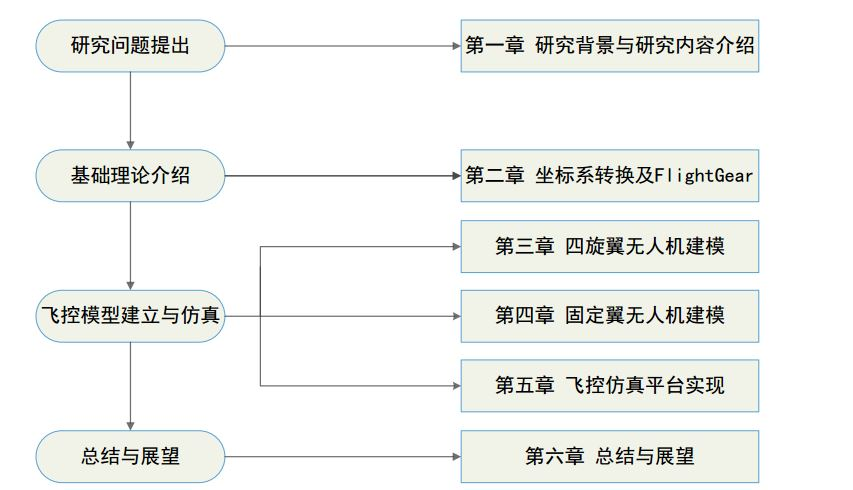
\includegraphics[width=0.8\textwidth]{f1.jpg}
\caption{论文结构 }
\label{fig1}
\end{figure}


第\ref{preface}章:主要介绍问题提出的研究背景,研究内容及研究目的,从宏观的角度对本文进行概括,对问题进行概述。

第\ref{introduction}章:推导四旋翼无人机坐标系变换公式与介绍FlightGear软件基础,,概述FlightGear 软件的运作流程。

第\ref{le}章:详细分析四旋翼无人机的飞控建模思路,首先,要通过编程实现飞行摇杆数据到飞控模型的数据传入,然后,通过建立的飞控模型,求解四旋翼无人机的飞行姿态参数,最后,传递给FlightGear进行视景模拟与仿真。

第\ref{routing}章:讲述固定翼无人机的飞控建模思路,第一步都是需要实现飞行摇杆的数据读入过程,固定翼无人机的飞控模型采用JSBSim 飞行动力学模型。通过模型求解,将飞机舵面参数,飞行姿态参数传递给FlightGear进行视景模拟与仿真。

第\ref{forward}章:通过前两章的建模与模型求解,在FlightGear飞行仿真平台上模拟仿真,实现飞行摇杆对无人机的飞行控制。同时,介绍FlightGear三维视景仿真系统的理论基础。

第\ref{conclusion}章:总结建模过程中的创新点与改进之处,提出进一步研究的方向与进度,对未来的研究工作提出展望。


\chapter{坐标系转换与FlightGear介绍}\label{introduction}
\section{坐标系转换\ucite{4}}
本文这一节主要介绍用于描述飞机姿态位置的坐标系与坐标系之间的转换,用来推导四旋翼飞控建模过程中需要用的旋转矩阵与转换方程。飞机的姿态描述需要利用各种坐标系表示的原因如下:
\begin{enumerate}
	\item 空气动力学的力和力矩是在机体坐标系下表示的。
	\item 牛顿运动方程利用四元数法来表示,需要指明相关的坐标系。
	\item 在机体坐标系下,飞机传感器读取飞机姿态参数信息,比如加速度;相反,飞机上GPS系统读取的飞机位置姿态参数需要在惯性坐标系下(即地面坐标系)。
	\item 大多数情况下,需要在惯性坐标系下,对飞机的飞行轨迹进行描述。另外,地图所采用的位置坐标也是在惯性坐标系下表示的。
\end{enumerate}

要想完成一个坐标系到另一个坐标系之间的转换,需要完成两个步骤,一个是旋转,另一个是转换。在本章的\ref{2.1.1}节部分用来描述坐标旋转矩阵和旋转矩阵应用于坐标系变化;在本章的\ref{2.1.2}节部分用来介绍在四旋翼无人机系统下所采用的特定坐标系,推导四旋翼旋转矩阵表达式;在本章的\ref{2.1.3}节部分用来推导坐标系转换过程中转换关系,即Corlios方程。最终,推导完成坐标系转换过程的两个步骤:旋转和转换。

\subsection{旋转矩阵理论基础}\label{2.1.1}
\begin{figure}[!ht]
\centering
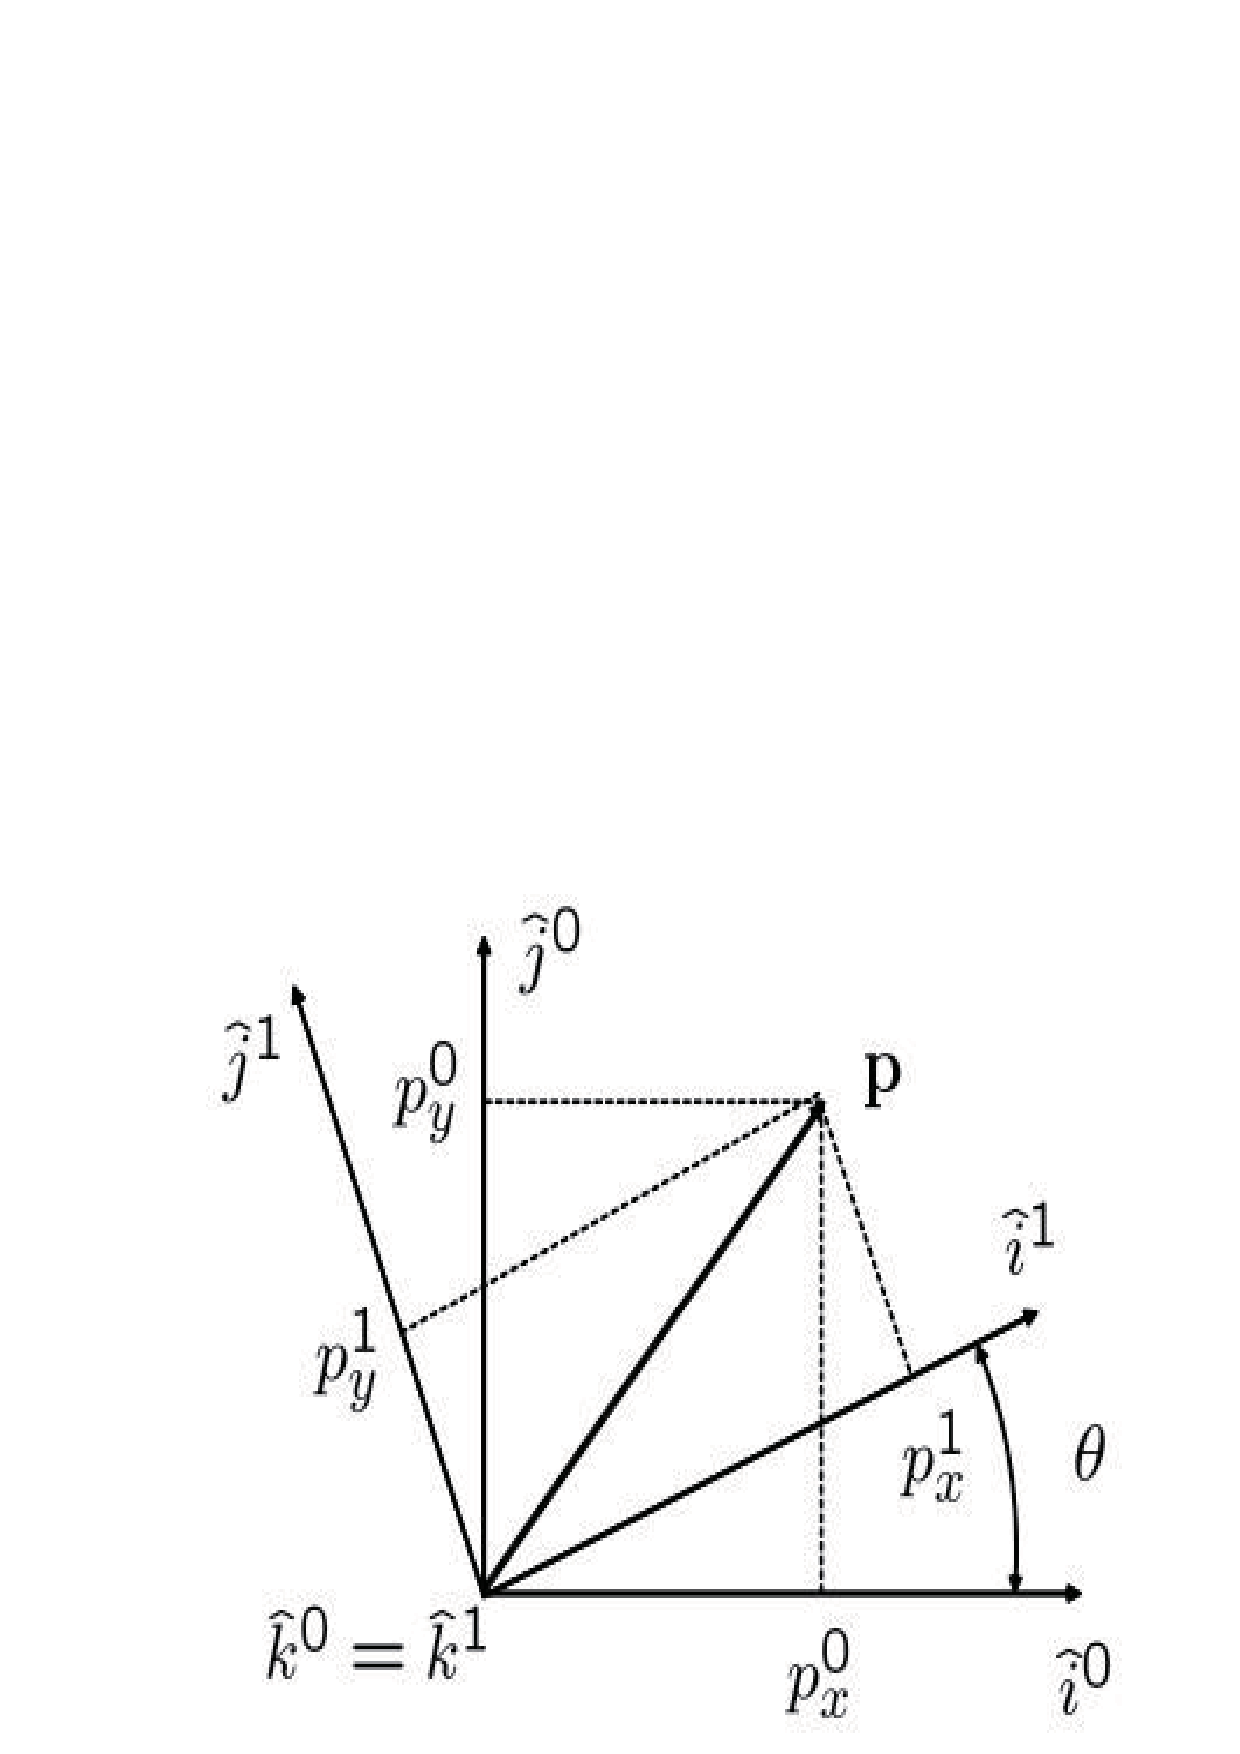
\includegraphics[width=0.6\textwidth]{f2.jpg}
\caption{坐标系二维旋转\ucite{4}}
\label{fig2}
\end{figure}
如图\ref{fig2}所示,向量{\bf{p}}即在坐标系$\mathop R\nolimits^0$下同时还在坐标系$\mathop R\nolimits^1$下,$\mathop R\nolimits^0$坐标系与$\mathop R\nolimits^1$坐标系的坐标原点相同,故向量{\bf{p}}从坐标系$\mathop R\nolimits^0$ 到坐标系$\mathop R\nolimits^1 $的旋转,属于二维空间的旋转。在坐标系$\mathop R\nolimits^0$下,单位向量用$\left( {{{\hat i}^0},{{\hat j}^0},{{\hat k}^0}} \right)$表示,在坐标系$\mathop R\nolimits^1 $下,单位向量用$\left( {{{\hat i}^1},{{\hat j}^1},{{\hat k}^1}} \right)$表示。在坐标系$\mathop R\nolimits^0$下,向量{\bf{p}}可以表示为:
\[\mathop {\bf{p}}\limits^{}  = \mathop p\nolimits_x^0 \mathop {\hat i}\nolimits^0  + \mathop p\nolimits_y^0 \mathop {\hat j}\nolimits^0  + \mathop p\nolimits_z^0 \mathop {\hat k}\nolimits^0 \]

同样,在坐标系系$\mathop R\nolimits^1 $下,向量{\bf{p}}可以表示为:
\[\mathop {\bf{p}}\limits^{}  = \mathop p\nolimits_x^1 \mathop {\hat i}\nolimits^1  + \mathop p\nolimits_y^1 \mathop
{\hat j}\nolimits^1  + \mathop p\nolimits_z^1 \mathop {\hat k}\nolimits^1 \]

联立上面两式,可以得到如下的关系:
\[\mathop p\nolimits_x^0 \mathop {\hat i}\nolimits^0  + \mathop p\nolimits_y^0 \mathop {\hat j}\nolimits^0  + \mathop p\nolimits_z^0 \mathop {\hat k}\nolimits^0  = \mathop p\nolimits_x^1 \mathop {\hat i}\nolimits^1  + \mathop p\nolimits_y^1 \mathop {\hat j}\nolimits^1  + \mathop p\nolimits_z^1 \mathop {\hat k}\nolimits^1 \]

上式两端分别点乘向量$\left( {{{\hat i}^1},{{\hat j}^1},{{\hat k}^1}} \right)$,通过化简可以表示为如下的形式:
\[\mathop {\bf{p}}\nolimits^{\bf{1}} {\kern 1pt} {\kern 1pt} {\kern 1pt} {\kern 1pt}  \buildrel \Delta \over = {\kern 1pt} {\kern 1pt} {\kern 1pt} {\kern 1pt} \left( \begin{array}{l}
\mathop p\nolimits_x^1 \\
\mathop p\nolimits_y^1 \\
\mathop p\nolimits_z^1
\end{array} \right) = \left( {\begin{array}{*{20}{c}}
{\mathop {\hat i}\nolimits^1  \cdot \mathop {\hat i}\nolimits^0 }&{\mathop {\hat i}\nolimits^1  \cdot \mathop {\hat j}\nolimits^0 }&{\mathop {\hat i}\nolimits^1  \cdot \mathop {\hat k}\nolimits^0 }\\
{\mathop {\hat j}\nolimits^1  \cdot \mathop {\hat i}\nolimits^0 }&{\mathop {\hat j}\nolimits^1  \cdot \mathop {\hat j}\nolimits^0 }&{\mathop {\hat j}\nolimits^1  \cdot \mathop {\hat k}\nolimits^0 }\\
{\mathop {\hat k}\nolimits^1  \cdot \mathop {\hat i}\nolimits^0 }&{\mathop {\hat k}\nolimits^1  \cdot \mathop {\hat j}\nolimits^0 }&{\mathop {\hat k}\nolimits^1  \cdot \mathop {\hat k}\nolimits^0 }
\end{array}} \right)\left( \begin{array}{l}
\mathop p\nolimits_x^0 \\
\mathop p\nolimits_y^0 \\
\mathop p\nolimits_z^0
\end{array} \right)\]

通过上式,结合图\ref{fig2}所示的几何关系,可以表示为如下的表达式:
\begin{equation}\label{1}
\mathop {\bf{P}}\nolimits^{\bf{1}}  = \mathop F\nolimits_0^1 \mathop {\bf{P}}\nolimits^{\bf{0}}
\end{equation}

其中,矩阵表示为从坐标系$\mathop R\nolimits^0$到坐标系$\mathop R\nolimits^1$的坐标旋转矩阵,$\theta$ 表示从坐标系$\mathop R\nolimits^0$的$x$轴逆时针旋转到坐标系$\mathop R\nolimits^1$的角度,旋转矩阵$\mathop F\nolimits_0^1 $用$\theta$角来表示,如下所示:
\[\mathop F\nolimits_0^1  = \left( {\begin{array}{*{20}{c}}
{\cos \left( \theta  \right)}&{\sin \left( \theta  \right)}&0\\
{ - \sin \left( \theta  \right)}&{\cos \left( \theta  \right)}&0\\
0&0&1
\end{array}} \right)\]

同理,若坐标系$\mathop R\nolimits^0$的$y$轴,按右手旋转法则转$\theta$角得到坐标系$\mathop R\nolimits^1$,旋转矩阵$\mathop F\nolimits_0^1 $用$\theta$角来表示:
\[\mathop F\nolimits_0^1  \buildrel \Delta \over = \left( {\begin{array}{*{20}{c}}
{\cos \left( \theta  \right)}&0&{ - \sin \left( \theta  \right)}\\
0&1&0\\
{\sin \left( \theta  \right)}&0&{\cos \left( \theta  \right)}
\end{array}} \right)\]

同理,若坐标系$\mathop R\nolimits^0$的$y$轴,按右手旋转法则转$\theta$角得到坐标系$\mathop R\nolimits^1$,旋转矩阵$\mathop F\nolimits_0^1 $用$\theta$角来表示:
\[\mathop F\nolimits_0^1  \buildrel \Delta \over = \left( {\begin{array}{*{20}{c}}
1&0&0\\
0&{\cos \left( \theta  \right)}&{\sin \left( \theta  \right)}\\
0&{ - \sin \left( \theta  \right)}&{\cos \left( \theta  \right)}
\end{array}} \right)\]

通过上面公式,我们可以得到旋转矩阵$\mathop F\nolimits_0^1 $重要的性质,如下所示:
\begin{itemize}
  \item ${\left( {\mathop F\nolimits_a^b } \right)^{{\rm{ - }}1}} = {\left( {\mathop F\nolimits_a^b } \right)^T} = \mathop F\nolimits_a^b $
  \item $\mathop F\nolimits_b^c \mathop F\nolimits_a^b  = \mathop F\nolimits_a^c $
  \item $\det \mathop F\nolimits_a^b  = 1$
\end{itemize}

\begin{figure}[!ht]
\centering
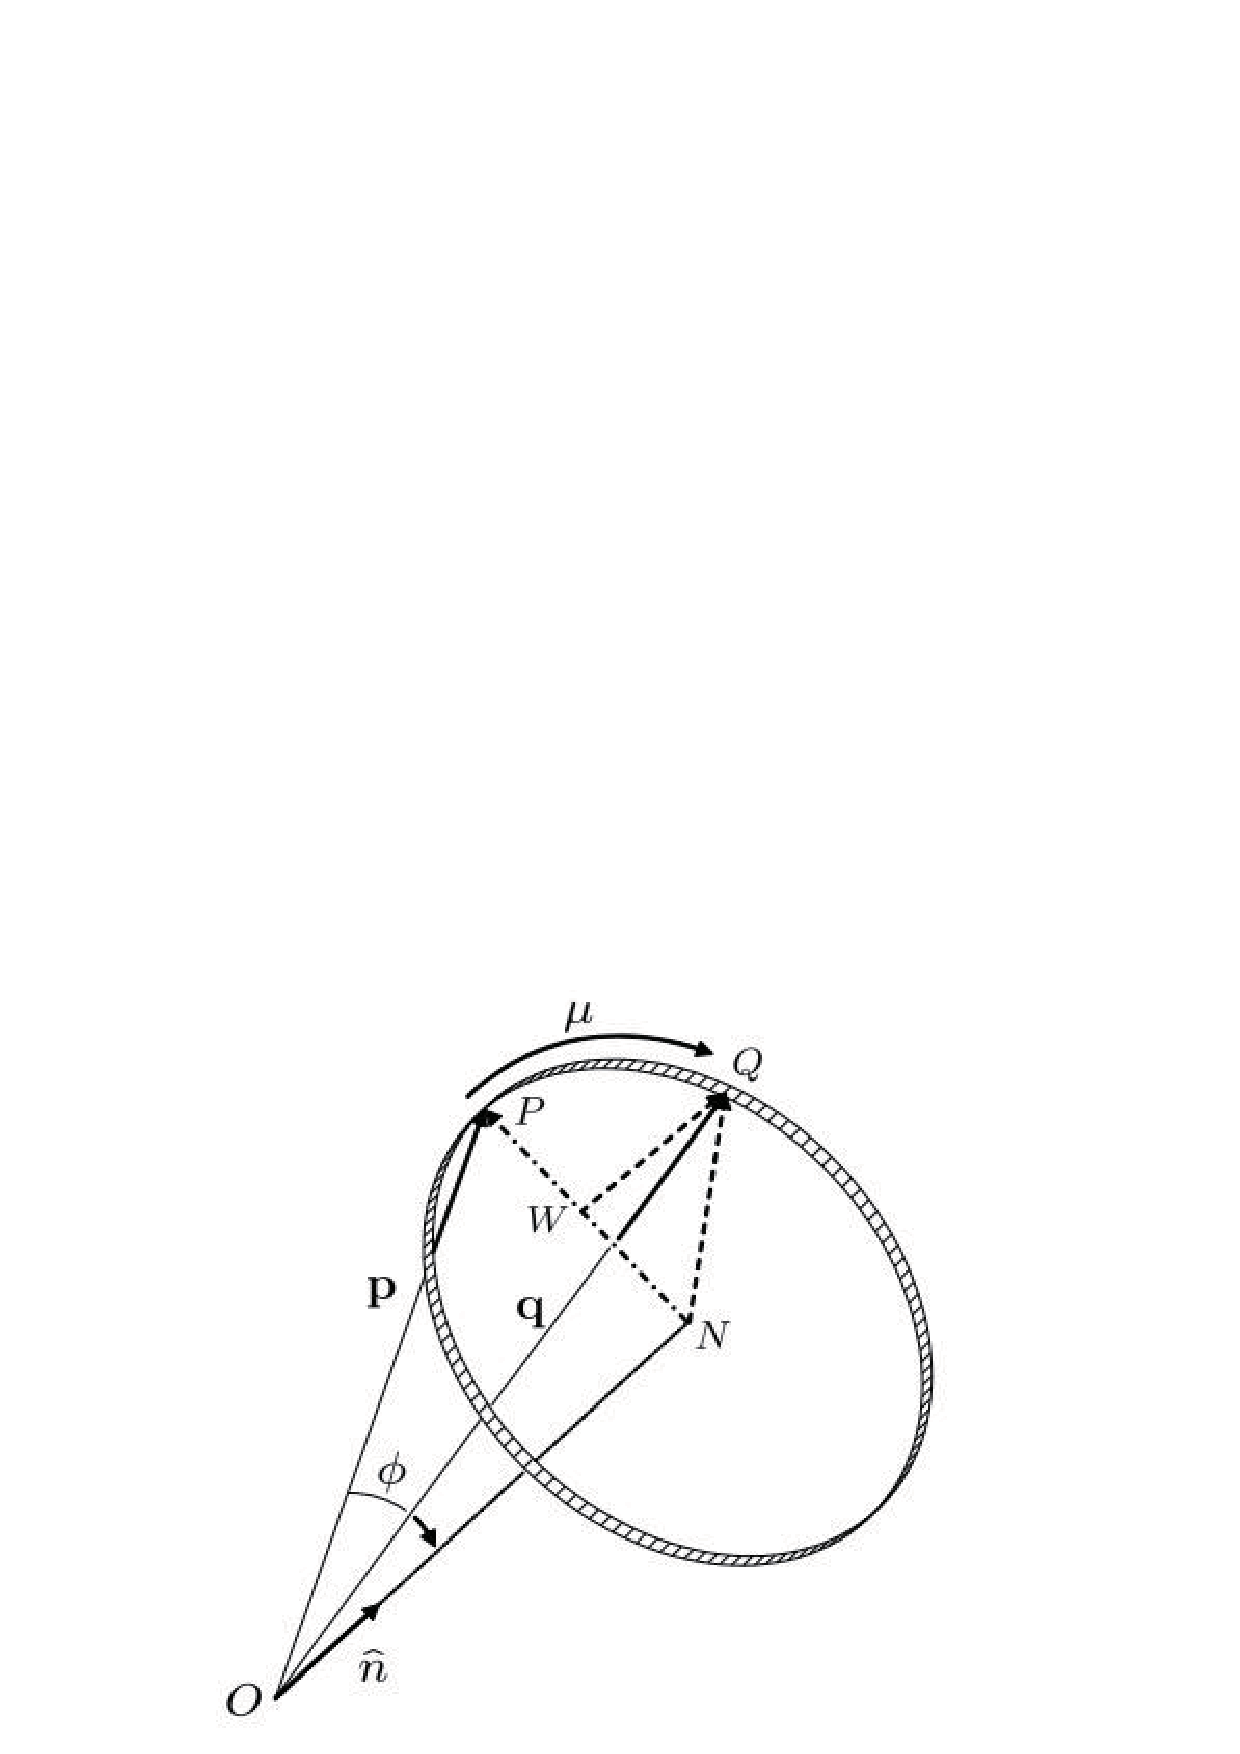
\includegraphics[width=0.6\textwidth]{f3.jpg}
\caption{旋转变换\ucite{4}}
\label{fig3}
\end{figure}

下面我们需要推导旋转公式,采用左手法则,如图\ref{fig3}所示,向量{\bf{p}}顺时针旋转$\mu$得到向量{\bf{q}},$\hat n$ 为单位向量。
\begin{equation}\label{2}
q = O\vec N + N\vec W + W\vec Q
\end{equation}

向量$O\vec N$可以用向量{\bf{p}}和单位向量{\bf{n}}来表示,向量{\bf{p}}在单位向量{\bf{n}}方向投影,得到向量$O\vec N$。
\[O\vec N{\rm{ = }}\left( {{\bf{p}} \cdot \hat n} \right)\hat n\]

向量$N\vec W$方向沿$\vec p - O\vec N$,长度由$NQ\cos \mu $表示。由图\ref{fig3}可知,$NQ$长度与$NP$长度相同,可以用$\left\| {\vec p - \left. {O\vec N} \right\|} \right.$来表示。
\[\begin{array}{l}
\displaystyle{N\vec W{\kern 1pt} {\kern 1pt} {\kern 1pt} {\kern 1pt} {\kern 1pt} {\kern 1pt}  = {\kern 1pt} {\kern 1pt} \frac{{{\bf{p}} - \left( {{\bf{p}} \cdot \hat n} \right)\hat n}}{{\left\| {{\bf{p}} - \left. {\left( {{\bf{p}} \cdot \hat n} \right)\hat n} \right\|} \right.}}}NQ\cos \mu \\
{\kern 1pt} {\kern 1pt} {\kern 1pt} {\kern 1pt} {\kern 1pt} {\kern 1pt} {\kern 1pt} {\kern 1pt} {\kern 1pt} {\kern 1pt} {\kern 1pt} {\kern 1pt} {\kern 1pt} {\kern 1pt} {\kern 1pt} {\kern 1pt} {\kern 1pt} {\kern 1pt} {\kern 1pt} {\kern 1pt} {\kern 1pt} {\kern 1pt} {\kern 1pt} {\kern 1pt} {\kern 1pt} {\kern 1pt} {\kern 1pt} {\kern 1pt} {\kern 1pt} {\kern 1pt} {\kern 1pt} {\kern 1pt} {\kern 1pt} {\rm{ = }}{\kern 1pt} {\kern 1pt} {\kern 1pt} \left( {{\bf{p}} - \left( {{\bf{p}} \cdot \hat n} \right)\hat n} \right)\cos \mu
\end{array}\]

向量$W\vec Q$方向垂直向量{\bf{p}}和{\bf{n}},长度由$NQ\sin \mu $表示。由图\ref{fig3}可知,$NQ$长度也可以用$\left\| {\vec p} \right\|\sin \phi $表示。
\[\begin{array}{l}
\displaystyle{W\vec Q{\kern 1pt} {\kern 1pt} {\kern 1pt} {\kern 1pt} {\rm{ = }}{\kern 1pt} {\kern 1pt} {\kern 1pt} {\kern 1pt} {\kern 1pt} \frac{{{\bf{p}} \times \hat n}}{{\left\| {\bf{p}} \right\|\sin \phi }}}NQ\sin \mu \\
{\kern 1pt} {\kern 1pt} {\kern 1pt} {\kern 1pt} {\kern 1pt} {\kern 1pt} {\kern 1pt} {\kern 1pt} {\kern 1pt} {\kern 1pt} {\kern 1pt} {\kern 1pt} {\kern 1pt} {\kern 1pt} {\kern 1pt} {\kern 1pt} {\kern 1pt} {\kern 1pt} {\kern 1pt} {\kern 1pt} {\kern 1pt} {\kern 1pt} {\kern 1pt} {\kern 1pt}  = {\kern 1pt}  - \hat n \times {\bf{p}}\sin \mu
\end{array}\]
因此,分别将向量$O\vec N$ ,向量$N\vec W$和向量$W\vec Q$表达式代入向量{\bf{q}}的表达式,得到旋转向量表达式,如下所示:
\begin{equation}\label{3}
{\bf{q}} = \left( {1 - \cos \mu } \right)\left( {{\bf{p}} \cdot \hat n} \right)\hat n + \cos \mu {\bf{p}} - \sin \mu \left( {\hat n \times {\bf{p}}} \right)
\end{equation}
\subsection{四旋翼旋转矩阵}\label{2.1.2}
在四旋翼飞行控制时,需要实现不同坐标系之间的转换,下面介绍常用的坐标系。
\subsubsection{惯性坐标系$\mathop R\nolimits^i $}
\begin{figure}[!ht]
\centering
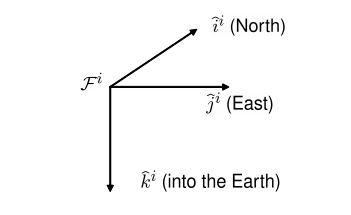
\includegraphics[width=0.4\textwidth]{f5.jpg}
\caption{惯性坐标系\ucite{4}}
\label{fig4}
\end{figure}
惯性坐标系是指坐标原点位于地心,如图\ref{fig4}所示,向量$\hat i$指向北,向量$\hat j$指向东,向量$\hat k$指向地心。
\subsubsection{速度坐标系$\mathop R\nolimits^\nu  $}
\begin{figure}[!ht]
\centering
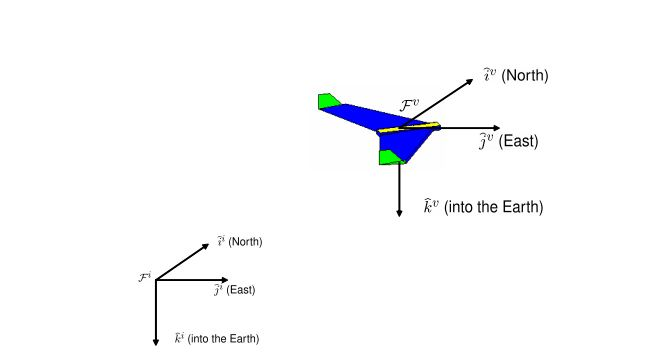
\includegraphics[width=0.9\textwidth]{f6.jpg}
\caption{速度坐标系\ucite{4}}
\label{fig5}
\end{figure}
坐标系的原点位于四旋翼的重心位置,$\mathop R\nolimits^\nu  $坐标系各轴的方向与惯性坐标系$\mathop R\nolimits^i $方向保持一致,如图\ref{fig5}所示。
\subsubsection{偏航坐标系$\mathop R\nolimits^{v1} $}
\begin{figure}[!ht]
\centering
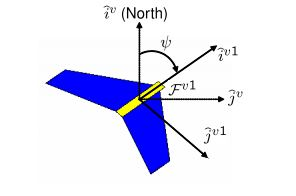
\includegraphics[width=0.6\textwidth]{f7.jpg}
\caption{偏航坐标系\ucite{4}}
\label{fig6}
\end{figure}
$\mathop R\nolimits^{v1} $坐标系的原点位于机体重心位置,$\mathop R\nolimits^{v1} $坐标系是机体绕$\mathop {\hat k}\nolimits^v $轴偏航$\psi $角,从而得到的偏航坐标系,即$\hat i$轴指向机头方向,$\hat j$轴指向右机翼方向,$\hat k$轴指向地心,如图\ref{fig6}所示。

由坐标系$\mathop R\nolimits^v $到坐标系$\mathop R\nolimits^{v1} $的转换,旋转角为$\psi $,利用前面推导的旋转矩阵公式可以得到:
\[\mathop {\bf{p}}\nolimits^{v1}  = \mathop F\nolimits_v^{v1} \left( \psi  \right)\mathop {\bf{p}}\nolimits^v \]

其中,\[\mathop F\nolimits_v^{v1} \left( \psi  \right){\rm{ = }}\left( {\begin{array}{*{20}{c}}
{\cos \psi }&{\sin \psi }&0\\
{ - \sin \psi }&{\cos \psi }&0\\
0&0&1
\end{array}} \right)\]
\subsubsection{俯仰坐标系$\mathop R\nolimits^{v2} $}
\begin{figure}[!ht]
\centering
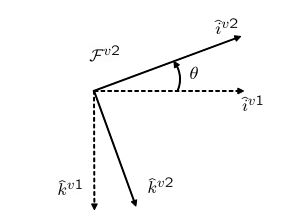
\includegraphics[width=0.6\textwidth]{f8.jpg}
\caption{俯仰坐标系\ucite{4}}
\label{fig7}
\end{figure}
$\mathop R\nolimits^{v2} $坐标系原点位于机体重心位置,$\mathop R\nolimits^{v2} $坐标系是$\mathop R\nolimits^v $坐标系绕$\mathop {\hat j}\nolimits^{v1} $轴俯仰$\theta $角,从而得到的俯仰坐标系,即$\hat i$轴指向机头方向,$\hat j$轴指向右机翼方向,$\hat k$轴指向机身下部。

由坐标系$\mathop R\nolimits^{v1} $到坐标系$\mathop R\nolimits^{v2} $的转换,旋转角为$\theta $,可得:
\[\mathop {\bf{p}}\nolimits^{v2}  = \mathop F\nolimits_{v1}^{v2} \left( \theta  \right)\mathop {\bf{p}}\nolimits^{v1} \]

其中,\[\mathop F\nolimits_{v1}^{v2} \left( \theta  \right) = \left( {\begin{array}{*{20}{c}}
{\cos \theta }&0&{ - \sin \theta }\\
0&1&0\\
{\sin \theta }&0&{\cos \theta }
\end{array}} \right)\]
\subsubsection{机体坐标系$\mathop R\nolimits^b $}
\begin{figure}[!ht]
\centering
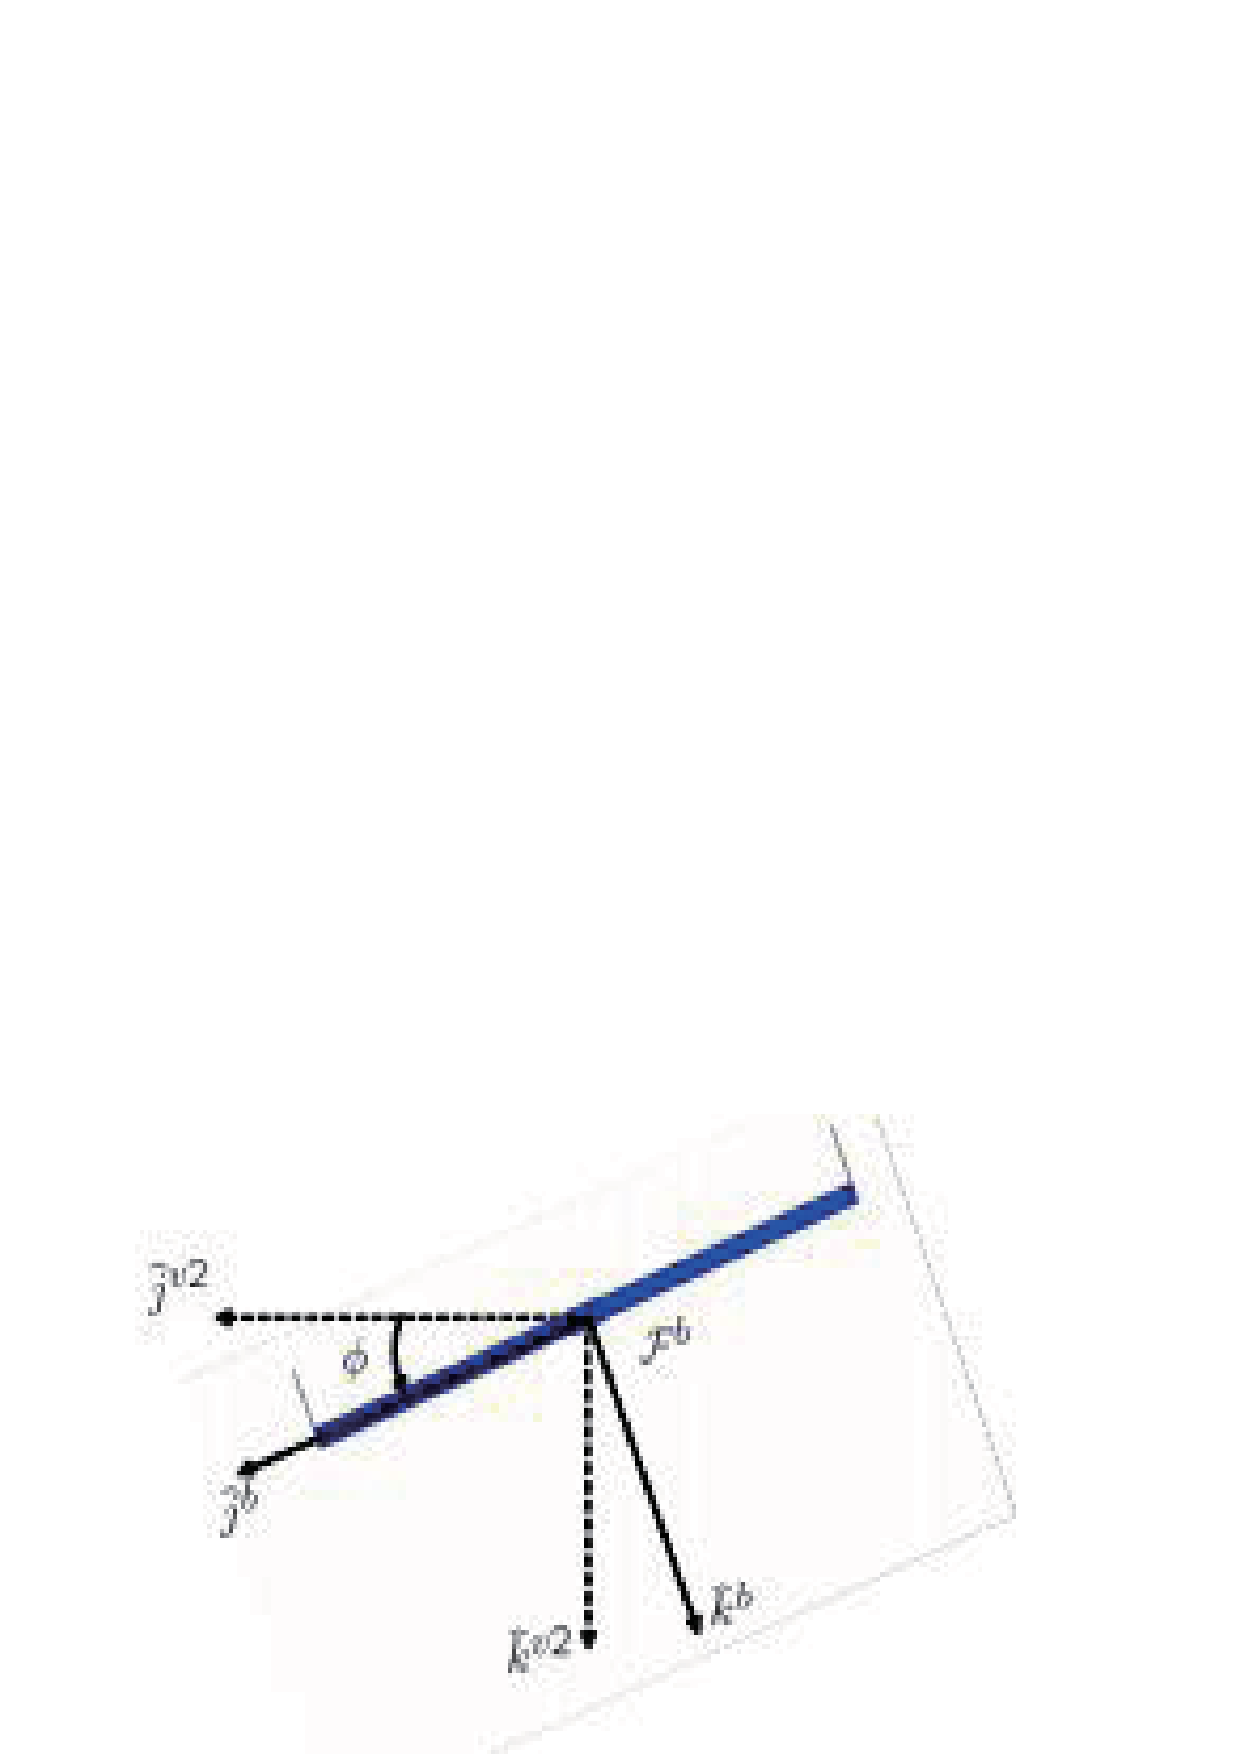
\includegraphics[width=0.6\textwidth]{f9.jpg}
\caption{机体坐标系\ucite{4}}
\label{fig8}
\end{figure}
机体坐标系通过$\mathop R\nolimits^{v2} $绕$\mathop {\hat i}\nolimits^{v2} $轴滚转$\phi $得到$\mathop R\nolimits^b $,如图\ref{fig8}所示。

由坐标系$\mathop R\nolimits^{v2} $到坐标系$\mathop R\nolimits^b $的转换,旋转角为$\phi $ ,可得:
\[\mathop {\bf{p}}\nolimits^b  = \mathop F\nolimits_{v2}^b \left( \phi  \right)\mathop {\bf{p}}\nolimits^{v2} \]

其中,\[\mathop F\nolimits_{v2}^b \left( \phi  \right) = \left( {\begin{array}{*{20}{c}}
1&0&0\\
0&{\cos \phi }&{\sin \phi }\\
0&{ - \sin \phi }&{\cos \phi }
\end{array}} \right)\]

因此,由$\mathop R\nolimits^v $到机体坐标系$\mathop R\nolimits^b $转换,得到的坐标系旋转矩阵。
\[\begin{array}{l}
\mathop F\nolimits_v^b \left( {\phi ,\theta ,\psi } \right) = \mathop F\nolimits_{v2}^b \left( \phi  \right)\mathop F\nolimits_{v1}^{v2} \left( \theta  \right)\mathop F\nolimits_v^{v1} \left( \psi  \right)\\
{\kern 1pt} {\kern 1pt} {\kern 1pt} {\kern 1pt} {\kern 1pt} {\kern 1pt} {\kern 1pt} {\kern 1pt} {\kern 1pt} {\kern 1pt} {\kern 1pt} {\kern 1pt} {\kern 1pt} {\kern 1pt} {\kern 1pt} {\kern 1pt} {\kern 1pt} {\kern 1pt} {\kern 1pt} {\kern 1pt} {\kern 1pt} {\kern 1pt} {\kern 1pt} {\kern 1pt} {\kern 1pt} {\kern 1pt} {\kern 1pt} {\kern 1pt} {\kern 1pt} {\kern 1pt} {\kern 1pt} {\kern 1pt} {\kern 1pt} {\kern 1pt} {\kern 1pt} {\kern 1pt} {\kern 1pt} {\kern 1pt} {\kern 1pt} {\kern 1pt} {\kern 1pt} {\kern 1pt} {\kern 1pt} {\kern 1pt} {\kern 1pt} {\kern 1pt} {\kern 1pt} {\kern 1pt} {\kern 1pt} {\kern 1pt} {\kern 1pt} {\kern 1pt} {\kern 1pt} {\kern 1pt} {\kern 1pt} {\kern 1pt} {\kern 1pt} {\kern 1pt}  = \left( {\begin{array}{*{20}{c}}
1&0&0\\
0&{\cos \phi }&{\sin \phi }\\
0&{ - \sin \phi }&{\cos \phi }
\end{array}} \right)\left( {\begin{array}{*{20}{c}}
{\cos \theta }&0&{ - \sin \theta }\\
0&1&0\\
{\sin \theta }&0&{\cos \theta }
\end{array}} \right)\left( {\begin{array}{*{20}{c}}
{\cos \psi }&{\sin \psi }&0\\
{ - \sin \psi }&{\cos \psi }&0\\
0&0&1
\end{array}} \right)\\
{\kern 1pt} {\kern 1pt} {\kern 1pt} {\kern 1pt} {\kern 1pt} {\kern 1pt} {\kern 1pt} {\kern 1pt} {\kern 1pt} {\kern 1pt} {\kern 1pt} {\kern 1pt} {\kern 1pt} {\kern 1pt} {\kern 1pt} {\kern 1pt} {\kern 1pt} {\kern 1pt} {\kern 1pt} {\kern 1pt} {\kern 1pt} {\kern 1pt} {\kern 1pt} {\kern 1pt} {\kern 1pt} {\kern 1pt} {\kern 1pt} {\kern 1pt} {\kern 1pt} {\kern 1pt} {\kern 1pt} {\kern 1pt} {\kern 1pt} {\kern 1pt} {\kern 1pt} {\kern 1pt} {\kern 1pt} {\kern 1pt} {\kern 1pt} {\kern 1pt} {\kern 1pt} {\kern 1pt} {\kern 1pt} {\kern 1pt} {\kern 1pt} {\kern 1pt} {\kern 1pt} {\kern 1pt} {\kern 1pt} {\kern 1pt} {\kern 1pt} {\kern 1pt} {\kern 1pt} {\kern 1pt} {\kern 1pt} {\kern 1pt} {\kern 1pt} {\kern 1pt} {\rm{ = }}\left( {\begin{array}{*{20}{c}}
{c\theta c\psi }&{c\theta s\psi }&{ - s\theta }\\
{s\phi s\theta c\psi  - c\phi s\psi }&{s\phi s\theta s\psi  + c\phi c\psi }&{s\phi c\theta }\\
{c\phi s\theta c\psi  + s\phi s\psi }&{c\phi s\theta s\psi  - s\phi c\psi }&{c\psi c\theta }
\end{array}} \right)
\end{array}\]

其中,$c\phi  \buildrel \Delta \over = \cos \phi $,$s\phi  \buildrel \Delta \over = \sin \phi $。
\subsection{Coriolis公式}\label{2.1.3}
在这一节,本文打算推导Coriolis数学关系式为后面飞控动力学关系作铺垫,Coriolis公式在坐标系变换过程中,起到非常重要的作用。假设,我们有两个坐标系,机体坐标系$\mathop R\nolimits^b $和惯性坐标系$\mathop R\nolimits^i $,如图\ref{fig9} 所示,向量${\bf{p}}$相对坐标系$\mathop R\nolimits^i $的运动,可以分解为两个运动,即:有向量${\bf{p}}$ 随着机体坐标系$\mathop R\nolimits^b $的平动,和向量${\bf{p}}$相对$\mathop R\nolimits^i $ 坐标系转动。
\begin{figure}[!ht]
\centering
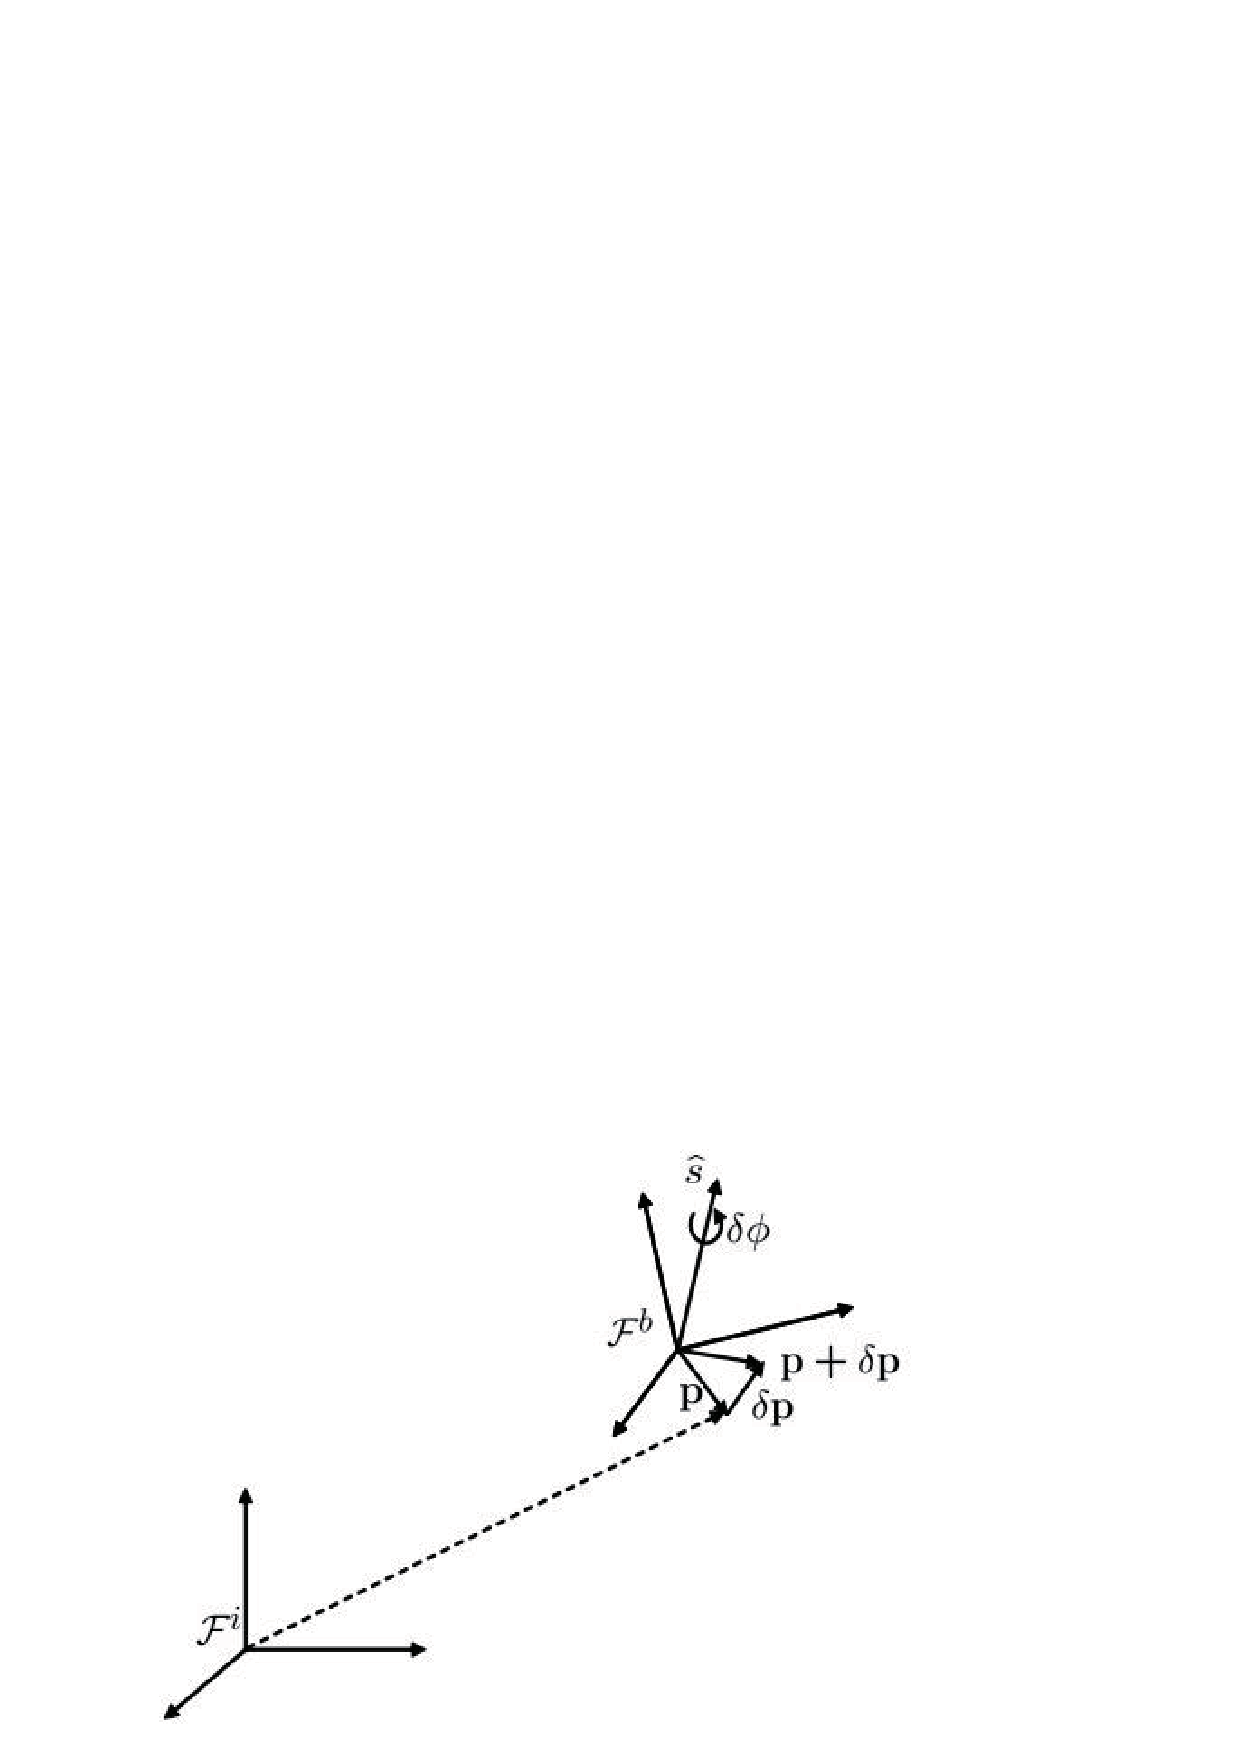
\includegraphics[width=0.6\textwidth]{f10.jpg}
\caption{Coriolis公式推导图\ucite{4}}
\label{fig9}
\end{figure}
下面总共两步推导Coriolis公式\ucite{15}:

\textbf{Step1:}

首先,假设机体坐标系$\mathop R\nolimits^b $不相对惯性坐标系$\mathop R\nolimits^i $转动,向量${\bf{p}}$随着向量机体坐标系$\mathop R\nolimits^b $ 平动,向量${\bf{p}}$相对惯性坐标系$\mathop R\nolimits^i $运动等价于向量${\bf{p}}$ 相对机体坐标系$\mathop R\nolimits^b $ 运动,如下所示:
\begin{equation}\label{4}
\frac{d}{{d{t_i}}}{\bf{p}} = \frac{d}{{d{t_b}}}{\bf{p}}
\end{equation}

\textbf{Step2:}

向量${\bf{p}}$静止在坐标系$\mathop R\nolimits^b $内,同时,坐标系$\mathop R\nolimits^b $相对坐标系$\mathop R\nolimits^i $ 转动,因此,向量${\bf{p}}$相对$\mathop R\nolimits^i $ 坐标系转动等效于坐标系$\mathop R\nolimits^b $相对坐标系$\mathop R\nolimits^i $转动,利用前面推导的旋转公式\ref{3},可得如下关系:
\[\vec p + \delta \vec p = \left( {1 - \cos \left( { - \delta \phi } \right)} \right)\hat s\left( {\hat s \cdot \vec p} \right) + \cos \left( { - \delta \phi } \right)\vec p - \sin \left( { - \delta \phi } \right)\hat s \times \vec p\]

利用小角度近似,同时等式两边同时除以$\delta t$,可得如下关系:
\[\frac{{\delta p}}{{\delta t}} \approx \frac{{\delta \phi }}{{\delta t}} \times \vec p\]

当$\delta t \to 0$时,$\mathop R\nolimits^b $坐标系相对$\mathop R\nolimits^i$坐标系的角速度可以表示为:${\omega _{b/i}} \buildrel \Delta \over = \hat s\dot \phi $,代入上式可得:
\begin{equation}\label{5}
{\frac{d}{{dt}}_i}{\bf{p}} = {\omega _{b/i}} \times {\bf{p}}
\end{equation}

因为,微分方程的线性性质,可以将公式\ref{4}和公式\ref{5}线性相加,便可得到Coriolis方程:
\begin{equation}
\frac{d}{{d{t_i}}}{\bf{p}} = \frac{d}{{d{t_b}}}{\bf{p}} + {\omega _{b/i}} \times {\bf{p}}
\end{equation}
\section{FlightGear软件介绍}
FlightGear是一个开源的飞行器模拟软件,由飞行模拟爱好者和编程爱好者共同合作开发的一款通过互联网提供大家学习的软件。FlightGear开发的原因一方面因为商业的飞行模拟软件价格高,受众群体小;另一方面,大多数商业的飞行模拟软件由于研发资金与开发时间的限制,并不能够提供一款功能全面的逼真的飞行模拟软件\ucite{8}。

\begin{figure}[!ht]
\centering
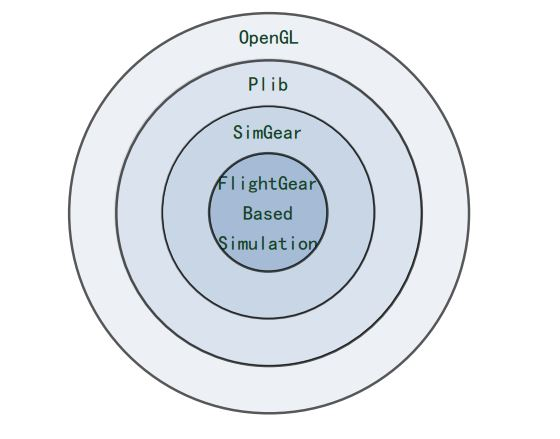
\includegraphics[width=0.5\textwidth]{f20.jpg}
\caption{FlightGear主要组件\ucite{9}}
\label{fig10}
\end{figure}
FlightGear作为一款大型的飞行模拟软件,结合了许多轻量级的开源软件。FlightGear主要使用的软件之间的关系如图\ref{fig10} 所示。下面分别介绍OpenGL, Plib和SimGear 在FlightGear功能实现过程中的功能与作用。
\begin{itemize}
  \item OpenGL

  OpenGL 是 Open Graphics Library 的缩写,意为开放的图形库,是 FlightGear最重要的组件。它是 SGI 公司开发的基于 FlightGear 的直升机飞行模拟系统研究的一套高性能图形处理系统,GL 代表图形库(Graphics  Library),前身是 SGI的 IRIX GL(工业标准 3D 计算机软件接口)\ucite{10}。OpenGL 是一个开放的三维图形软件包,具有强大图形处理功能,提供了基本库、实用库、辅助库,包含 100 多个函数,能够构建三维场景并对三维模型进行渲染着色,使三维模型更加逼真\ucite{11,12}。
  \item SimGear

SimGear 是仿真架构的开源工具集,是 FlightGear 的仿真引擎,主要功能模块介绍如表\ref{t1}所示\ucite{8}。
\vspace{-10pt}
\begin{table}[!h]
\begin{center}
\caption{SimGear功能模块介绍}\label{t1}
\begin{longtable}{ | c| c|}
\hline
模块名称                                    & 功能描述                                                                   \\\hline
SGBucket                     & 负责管理世界地图场景                                     \\\hline
SGDebug           & 用于程序调试,跟踪软件运行情况                                        \\\hline
SGEphem                   & 管理星历表,以便准确渲染这些天体                                                 \\\hline
SGIO                      & 与底层 I/O 的接口驱动,如 socket、串行端口等
                                          \\\hline
SGMagVar                 & 利用地理坐标和时间计算磁变值和磁倾角,为飞行器助航
                          \\\hline
SGMath  &  提供矢量计算、坐标变换、随机数产生等数学函数
 \\\hline
SGEnvironment             & 提供与天气环境相关的一些辅助类
\\\hline
SGMisc  &提供混杂的一些工具库,如管理文件路径的 SGPath 类
\\\hline
SGNasal &提供 nasal“脚本”语言
\\\hline
SGProps &FlightGear 数据结构的核心功能
\\\hline
SGRoute &管理单个或一系列航路点,用于自动驾驶模块的导航
\\\hline
SGMaterial&管理场景图形的材质资源
\\\hline
SGModel &管理 3D 模型
\\\hline
SGSky &模拟真实飞行中的天空环境
\\\hline
SGSound &音效模块,对 OpenAL 进行了封装,管理所有的声音信息
\\\hline
SGTiming &时间分系统,计算管理各种时间参数
\\\hline
SGXML &解析 XML 文档
\\\hline
\end{longtable}
\end{center}
\end{table}
\vspace{-10pt}

FlightGear开发正是弥补以上的飞行模拟软件的缺陷,通过表\ref{t1}所示,强大的仿真引擎功能,从而提供更加友好的用户界面,满足飞行模拟爱好者对飞行的热爱。因此,FlightGear具有以下的优势 \ucite{8}:
\begin{enumerate}
  \item 跨平台性:FlightGear支持Linux, Windows, Mac OS X等多个操作系统,为了满足用户在多个操作系统或者平台上使用FlightGear飞行模拟软件。
  \item 开源性:FlightGear开源性,支持任何人对FlightGear软件的改善,同时,分享FlightGear软件的所有源代码文件,为科研学术研究提供更好的平台。
  \item 可拓展性:FlightGear开发者们意在提供一个可以满足任何用户需求的飞行模拟软件,与其他商业的飞行模拟软件不同,FlightGear所有的文件都是免费提供给用户可见的,任何人都可以看FlightGear是如何编码开发的,目的就是让更多的用户使用这款飞行模拟软件。从设计之初开始,FlightGear 的场景地形、内部参数、API 函数和其它任何模块都对用户透明以及有文档记录。用户可以根据自身需求对 FlightGear 软件进行扩展设计,实现新的功能。
\end{enumerate}
  \item Plib

  Plib(Portable Game Libraries)也是一个开源库,由 Steve J. Baker 开发维护,包含 GUI、3D、音效、窗口管理等。Plib 包同样具有跨平台性,支持 Linux、Windows、Mac OS 等操作系统,各功能模块之间如表\ref{t2}所示\ucite{13}。
  \vspace{-10pt}
  \begin{table}[h]
\begin{center}
\caption{Plib功能模块介绍}\label{t2}
\begin{longtable}{ | c| p{5cm}|}
\hline
模块名称                                    & 功能描述                                                                   \\\hline
UL(Utility Library)                     & 隐藏操作系统之间的差异,使函数通用,为其他库提供
辅助类或例行程序                                     \\\hline
SG(Standard Geometry Library)           & 为提高 OpenGL 运行效率而写的一个简单的矩阵和矢
量数学库,在 Plib 其他部分中大量运用
                                       \\\hline
JS(Joystick Wrappers)                   & 封装操纵杆,支持更多操纵杆、轴、按钮
                                                    \\\hline
FNT(Font Library)                       & 封装字体,将输入文本映射为纹理在 OpenGL 里绘制                                          \\\hline
SSG(Simple Scene Graph)                 & 简单场景图形,设计为一个相对简单的、轻负载的构建
在 OpenGL 层之上的场景图形 API
                         \\\hline
PUI (Picoscopic User Interface Library) &  一组需要 OpenGL 和 C++操作的 GUI 窗口小部件(如
菜单、按钮、组合框、标签、滚动条等),在 3D 硬件
上的执行速度非常快
 \\\hline
NET(Pegasus Network Library)            & 一个封装了联网功能的 C++库,在游戏中加入网络功能
将变得非常容易,使用 NET 前,要首先调用 netInit 函
数。

\\\hline
\end{longtable}
\end{center}
\end{table}
\end{itemize}
\vspace{-10pt}
\subsection{FlightGear程序架构}
\vspace{10pt}
由上一节可以知道,FlightGear以SimGear为仿真引擎,由OpenGL处理图像,Open AL处理音频,Plib实现跨平台,网络通信等辅助功能的飞行模拟软件。本节主要来介绍FlightGear的程序架构,分为两部分来介绍,一部分是框架结构,另一部分是运行流程,来了解FlightGear各个子系统之间的关系与功能。
\subsubsection{FlightGear框架结构}
\vspace{10pt}
FlightGear由飞行动力学系统,控制系统,飞行器模块,时间系统,场景系统等子系统构成,各个子系统之间的关系并不是相互独立,而是相互联系的,子系统之间的关系如\ref{fig11}所示\ucite{13}。
\begin{figure}[!ht]
\centering
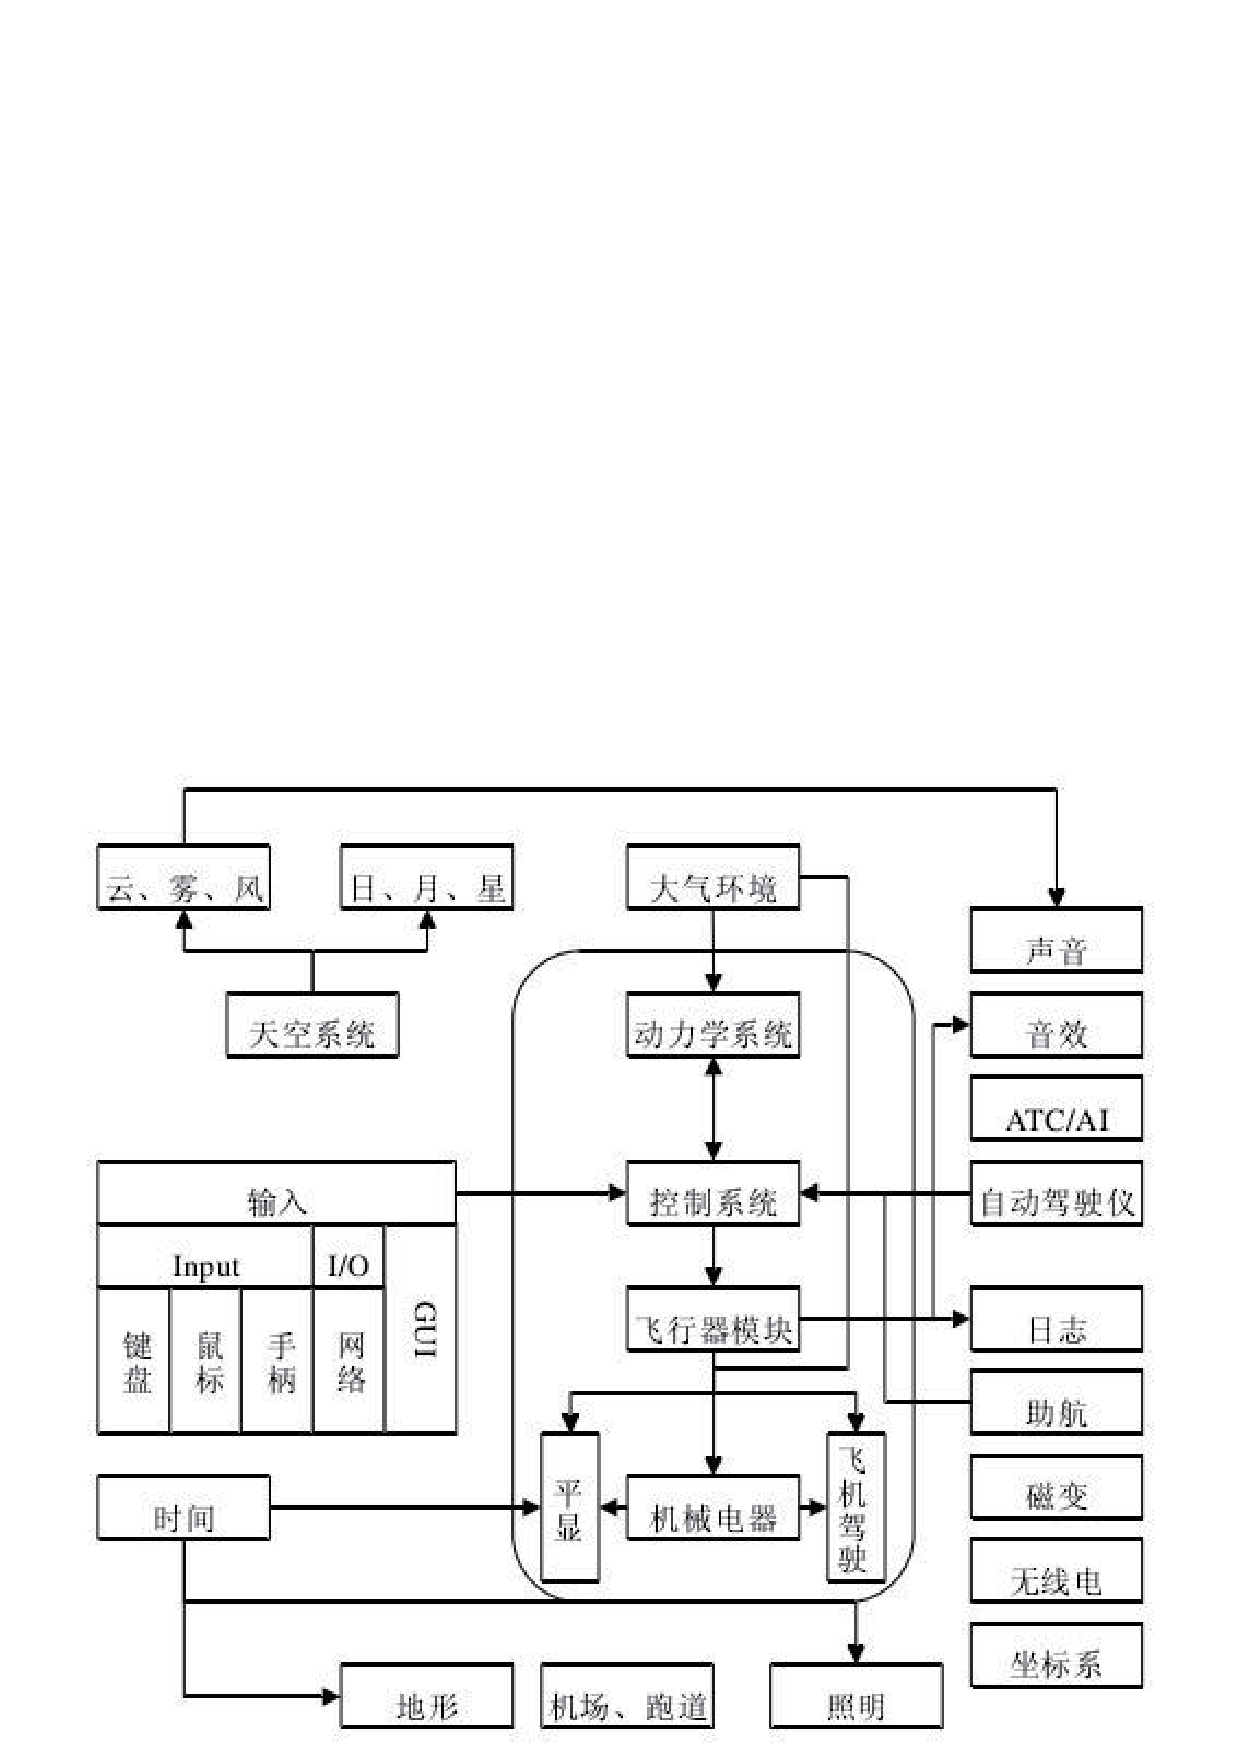
\includegraphics[width=1.0\textwidth]{f15.jpg}
\caption{FlightGear主要组件\ucite{13}}
\label{fig11}
\end{figure}
\subsection{ FlightGear 运行流程}
FlightGear使用C++语言开发,其运行流程如图\ref{fig12}所示\ucite{14}。由图\ref{fig12}可知,FlightGear运行流程主要有两个主循环构成,主循环1 负责完成各个模块的初始化功能。初始化功能通过变量$Idle\_State$累加来控制,随着控制参数$Idle\_State$参数迭代累加的过程,完成各个模块的初始化,主要是助航系统初始化、三维飞行器模型、环境模型(包括天空模型)、OpenGL参数设置,SSG 模块的初始化。同时,主循环1 过程中的窗口系统只要用来完成启动界面的渲染功能。

由图\ref{fig12}可知,在主循环2的过程中,主要完成整个系统更新的功能,是
FlightGear运行过程的核心部分,在该循环过程中的窗口系统则主要用来完成三维化可视仿真系统中的渲染功能\ucite{14},主要针对天空,飞行器,地面等场景的渲染。
\begin{figure}[!ht]
\centering
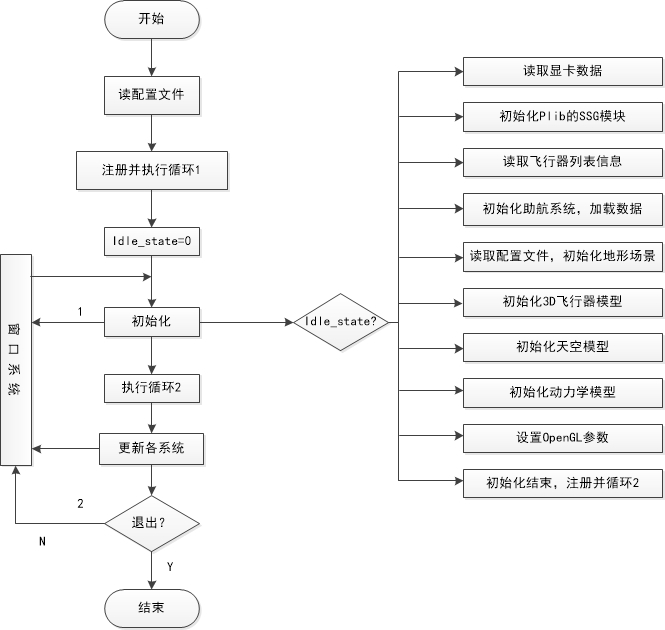
\includegraphics[width=1.0\textwidth]{f16.jpg}
\caption{FlightGear主要组件\ucite{14}}
\label{fig12}
\end{figure}

\chapter{四旋翼无人机飞控建模}\label{le}
在本章,本文分三部分介绍四旋翼的飞控建模过程,\ref{1}节是飞行摇杆的数据传入过程,作为四旋翼无人机的姿态角的输入;\ref{2}节 是四旋翼无人机飞行动力学部分,也是本章的核心部分;\ref{3}节是三维视景系统的设计原理。关系如图\ref{fig17}所示。
\vspace{-10pt}
\begin{figure}[!ht]
\centering
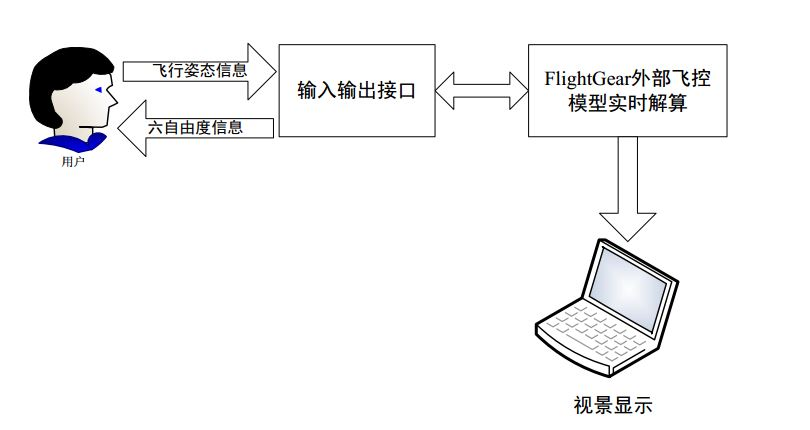
\includegraphics[width=0.8\textwidth]{f18.jpg}
\caption{四旋翼飞控建模过程}
\label{fig17}
\end{figure}
\vspace{-10pt}
\section{飞行摇杆数据传入}\label{1}
  本文将飞行摇杆(Joystick)数据读取作为四旋翼飞控模型的输入,Joystick数据的数据主要是四旋翼的姿态角(滚转角,偏航角,俯仰角)和四旋翼的推力。因此,本文通过C++编程,实现飞行摇杆数据的输入。由如下代码所示:

 \begin{lstlisting}[language={[ANSI]C++}]
class HAL_JoyStick: public ZY::Thread {
public:
    HAL_JoyStick(){
        m_devID = -1;
    }
    HAL_JoyStick(int dev) {
        m_devID=dev;
    }
    virtual ~HAL_JoyStick() {}
    int open(int devID);
    void run();
    int close(void);
    int read(JS_Val *jsv)
    {
        data_mutex.lock();
        *jsv= m_JSVal;
        m_JSVal.dataUpdated = 0;
        data_mutex.unlock();
        return 0;
    }
public:
    int         m_devType;
    int         m_devID;
    int         m_devFD;
    char        number_of_axes;
    char        number_of_btns;
protected:
    ZY::Mutex   data_mutex;
    JS_Val      m_JSVal;
}
\end{lstlisting}

\section{四旋翼飞控建模\ucite{4}}\label{2}
在本节中,分为三部分进行四旋翼飞行动力学建模的过程,第一部分是四旋翼飞行建模中需要的变量与坐标系的说明与定义;第二部分是推导六自由度四旋翼飞行动力学方程;第三部分是对模型进行化简,进行模型的求解。
  \subsection{四旋翼变量}
\begin{table}[!h]
\begin{center}
\caption{四旋翼参数表}\label{t1}
\begin{longtable}{ | c| c|}
\hline
参数名称                                    & 参数意义                                                                  \\\hline
${p_n}$                    & 惯性坐标系$\mathop R\nolimits^i $下,四旋翼$x$轴方向的位置                               \\\hline
${p_e}$           & 惯性坐标系$\mathop R\nolimits^i $下,四旋翼$y$轴方向的位置                                    \\\hline
$h$              & 惯性坐标系$\mathop R\nolimits^i $下, 四旋翼$z$轴方向的高度                                            \\\hline
$u$                      & 机体坐标系$\mathop R\nolimits^b $下,四旋翼$x$轴方向的速度
                                          \\\hline
$v$                 & 机体坐标系$\mathop R\nolimits^b $下,四旋翼$y$轴方向的速度
                          \\\hline
$\omega $ &  机体坐标系$\mathop R\nolimits^b $下,四旋翼$z$轴方向的速度
 \\\hline
$\phi $             & 滚转角
\\\hline
$\theta $ &俯仰角
\\\hline
$\psi $  &  偏航角
\\\hline
$p$ &   机体坐标系$\mathop R\nolimits^b $下,滚转角速率
\\\hline
$q$ &  机体坐标系$\mathop R\nolimits^b $下,俯仰角速率
\\\hline
$r$ &    机体坐标系$\mathop R\nolimits^b $下,偏航角速率
\\\hline
\end{longtable}
\end{center}
\end{table}
\vspace{-20pt}
如表\ref{t1}所示,四旋翼建模过程中所需的参数变量,将上述变量关系在图\ref{fig19}中所示。四旋翼姿态位置变量$\left( {{p_n},{p_e},h} \right)$是定义在惯性坐标系(即地面坐标系)下,其中,高度变量$h$在惯性坐标系下沿着$z$轴的负半轴方向,即方向向上。在机体坐标系下,定义四旋翼的速度变量$\left( {u,v,\omega } \right)$和角速度变量$\left( {p,q,r} \right)$。欧拉角(滚转角$\phi $,俯仰角$\theta $,$\psi $)分别定义与上章的滚转坐标系,俯仰坐标系和偏航坐标系下。

\begin{figure}[!ht]
\centering
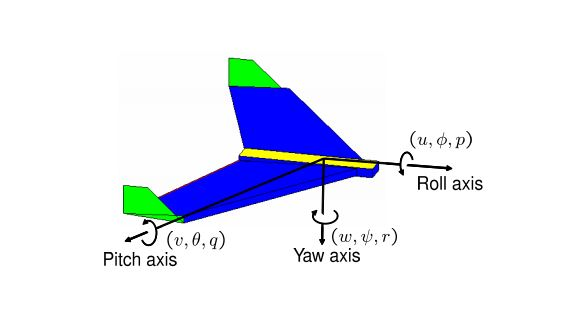
\includegraphics[width=0.7\textwidth]{f19.jpg}
\caption{坐标轴定义}
\label{fig19}
\end{figure}

  \subsection{四旋翼六自由度飞行动力学建模}
  \subsubsection{四旋翼运动学方程}
	在地面坐标系下,定义四旋翼姿态位置变量$\left( {{p_n},{p_e},h} \right)$;在机体坐标系下,定义四旋翼速度变量$\left( {u,v,\omega } \right)$。因此,需要建立位置变量与姿态变量之间的关系,结合2.1节坐标系转换的公式可得:

\[\begin{array}{l}
\frac{d}{{dt}}\left( \begin{array}{l}
{p_n}\\
{p_e}\\
 - h
\end{array} \right) = \mathop F\nolimits_b^v \left( \begin{array}{l}
u\\
v\\
\omega
\end{array} \right)\\
{\kern 1pt} {\kern 1pt} {\kern 1pt} {\kern 1pt} {\kern 1pt} {\kern 1pt} {\kern 1pt} {\kern 1pt} {\kern 1pt} {\kern 1pt} {\kern 1pt} {\kern 1pt} {\kern 1pt} {\kern 1pt} {\kern 1pt} {\kern 1pt} {\kern 1pt} {\kern 1pt} {\kern 1pt} {\kern 1pt} {\kern 1pt} {\kern 1pt} {\kern 1pt} {\kern 1pt} {\kern 1pt} {\kern 1pt} {\kern 1pt} {\kern 1pt} {\kern 1pt} {\kern 1pt} {\kern 1pt} {\kern 1pt} {\kern 1pt} {\kern 1pt} {\kern 1pt} {\kern 1pt} {\kern 1pt} {\kern 1pt} {\kern 1pt} {\kern 1pt} {\kern 1pt} {\kern 1pt} {\kern 1pt} {\kern 1pt} {\kern 1pt} {\kern 1pt} {\kern 1pt} {\kern 1pt} {\kern 1pt} {\kern 1pt} {\kern 1pt} {\kern 1pt} {\kern 1pt} {\kern 1pt} {\kern 1pt} {\kern 1pt} {\kern 1pt} {\kern 1pt} {\kern 1pt}  = {\left( {\mathop F\nolimits_b^v } \right)^T}\left( \begin{array}{l}
u\\
v\\
\omega
\end{array} \right)\\
{\kern 1pt} {\kern 1pt} {\kern 1pt} {\kern 1pt} {\kern 1pt} {\kern 1pt} {\kern 1pt} {\kern 1pt} {\kern 1pt} {\kern 1pt} {\kern 1pt} {\kern 1pt} {\kern 1pt} {\kern 1pt} {\kern 1pt} {\kern 1pt} {\kern 1pt} {\kern 1pt} {\kern 1pt} {\kern 1pt} {\kern 1pt} {\kern 1pt} {\kern 1pt} {\kern 1pt} {\kern 1pt} {\kern 1pt} {\kern 1pt} {\kern 1pt} {\kern 1pt} {\kern 1pt} {\kern 1pt} {\kern 1pt} {\kern 1pt} {\kern 1pt} {\kern 1pt} {\kern 1pt} {\kern 1pt} {\kern 1pt} {\kern 1pt} {\kern 1pt} {\kern 1pt} {\kern 1pt} {\kern 1pt} {\kern 1pt} {\kern 1pt} {\kern 1pt} {\kern 1pt} {\kern 1pt} {\kern 1pt} {\kern 1pt} {\kern 1pt} {\kern 1pt} {\kern 1pt} {\kern 1pt} {\kern 1pt} {\kern 1pt} {\kern 1pt}  = \left( {\begin{array}{*{20}{c}}
{c\theta c\psi }&{s\phi s\theta c\psi  - c\phi s\psi }&{c\phi s\theta c\psi  + s\theta s\psi }\\
{c\theta s\psi }&{s\phi s\theta s\psi  + c\phi c\psi }&{c\phi s\theta s\psi  - s\theta c\psi }\\
{ - s\theta }&{s\phi c\theta }&{c\phi c\theta }
\end{array}} \right)\left( \begin{array}{l}
u\\
v\\
\omega
\end{array} \right)
\end{array}\]

其中,$c = \cos {\kern 1pt} ,s = \sin $。

同样,欧拉角(滚转角$\phi $,俯仰角$\theta $,$\psi $)和角速度$\left( {p,q,r} \right)$之间也需要坐标系的转换。但是,它们之间坐标系的转换是复杂的,角速度变量被定义于机体坐标系,但是,欧拉角分别定义于三个不同的坐标系,即滚转角坐标系,俯仰角坐标系和偏航角坐标系(2.1节所示)。于是,我们需要建立起角速度$\left( {p,q,r} \right)$和欧拉角速率$\left( {\mathop \phi \limits^ \cdot  ,\mathop \theta \limits^ \cdot  ,\mathop \psi \limits^ \cdot  } \right)$之间的关系。因为欧拉角速率均为小量,可以近似于欧拉角与角速度之间的关系。
\[\mathop F\nolimits_{v2}^b \left( {\mathop \phi \limits^ \cdot  } \right) = \mathop F\nolimits_{v1}^{v2} \left( {\mathop \theta \limits^ \cdot  } \right) = \mathop F\nolimits_v^{v1} \left( {\mathop \psi \limits^ \cdot  } \right)\]
因此,我们可以得到:
\small
\begin{equation}
\begin{array}{l}
\left( \begin{array}{l}
p\\
q\\
r
\end{array} \right) = \mathop R\nolimits_{v2}^b \left( {\mathop \phi \limits^ \cdot  } \right)\left( \begin{array}{l}
\mathop \phi \limits^ \cdot  \\
0\\
0
\end{array} \right) + \mathop R\nolimits_{v2}^b \left( \phi  \right)\mathop R\nolimits_{v1}^{v2} \left( {\mathop \theta \limits^ \cdot  } \right)\left( \begin{array}{l}
0\\
\mathop \theta \limits^ \cdot  \\
0
\end{array} \right) + \mathop R\nolimits_{v2}^b \left( \phi  \right)\mathop R\nolimits_{v1}^{v2} \left( {\mathop \theta \limits^ \cdot  } \right)\mathop R\nolimits_{v \to v1} \left( {\mathop \psi \limits^ \cdot  } \right)\left( \begin{array}{l}
0\\
0\\
\mathop \psi \limits^ \cdot
\end{array} \right)\\
{\kern 1pt}  = \left( \begin{array}{l}
\mathop \phi \limits^ \cdot  \\
0\\
0
\end{array} \right) + \left( {\begin{array}{*{20}{c}}
1&0&0\\
0&{\cos \phi }&{\sin \phi }\\
0&{ - \sin \phi }&{\cos \phi }
\end{array}} \right)\left( \begin{array}{l}
0\\
\mathop \theta \limits^ \cdot  \\
0
\end{array} \right) + \left( {\begin{array}{*{20}{c}}
1&0&0\\
0&{\cos \phi }&{\sin \phi }\\
0&{ - \sin \phi }&{\cos \phi }
\end{array}} \right)\left( {\begin{array}{*{20}{c}}
{\cos \theta }&0&{ - \sin \theta }\\
0&1&0\\
{\sin \theta }&0&{\cos \theta }
\end{array}} \right)\\
 = \left( {\begin{array}{*{20}{c}}
1&0&{ - s\theta }\\
0&{{\mathop{\rm c}\nolimits} \phi }&{{\mathop{\rm s}\nolimits} \phi c\theta }\\
0&{ - {\mathop{\rm s}\nolimits} \phi }&{c\phi c\theta }
\end{array}} \right)\left( \begin{array}{l}
\mathop \phi \limits^ \cdot  \\
\mathop \theta \limits^ \cdot  \\
\mathop \psi \limits^ \cdot
\end{array} \right)
\end{array}
\end{equation}
\small
通过,对上式求逆可得:
\begin{equation}
\left( \begin{array}{l}
\mathop \phi \limits^ \cdot  \\
\mathop \theta \limits^ \cdot  \\
\mathop \psi \limits^ \cdot
\end{array} \right) = \left( {\begin{array}{*{20}{c}}
1&{\sin \left( \phi  \right)\tan \left( \theta  \right)}&{\cos \left( \phi  \right)\tan \left( \theta  \right)}\\
0&{\cos \left( \phi  \right)}&{ - \sin \left( \phi  \right)}\\
0&{\sin \left( \phi  \right)\sec \left( \theta  \right)}&{\cos \left( \phi  \right)\sec \left( \theta  \right)}
\end{array}} \right)\left( \begin{array}{l}
p\\
q\\
r
\end{array} \right)
\end{equation}

在惯性坐标系下,根据牛顿第二定律的微分形式,可以得到四旋翼的速度与力之间的关系,如下所示:
\[m\frac{{d{\bf{v}}}}{{d{t_i}}} = {\bf{f}}\]

其中,$m$是四旋翼的质量,${\bf{f}}$是四旋翼的合力,$\frac{d}{{d{t_i}}}$是四旋翼在惯性坐标系下的时间导数。根据2.1.3节的Coriolis公式可得:
\begin{equation}
m\frac{{d{\bf{v}}}}{{d{t_i}}} = m\left( {\frac{{d{\bf{v}}}}{{d{t_b}}} + {\omega _{b/i}} \times {\bf{v}}} \right) = {\bf{f}}
\end{equation}

其中,${\omega _{b/i}}$是在惯性坐标系下的角速度,因为四旋翼的受力是在机体坐标系下计算的,所以,$\omega$在机体坐标系下进行测量,利用上式,结合${{\bf{v}}^b} \buildrel \Delta \over = {\left( {u,v,\omega } \right)^T}$和${\omega _{b/i}} \buildrel \Delta \over = {\left( {p,q,r} \right)^T}$关系式以及${{\bf{f}}^b} \buildrel \Delta \over = {\left( {{f_x},{f_y},{f_z}} \right)^T}$上式可以表示为:
\begin{equation}
\left( \begin{array}{l}
\mathop u\limits^ \cdot  \\
\mathop \nu \limits^ \cdot  \\
\mathop \omega \limits^ \cdot
\end{array} \right) = \left( \begin{array}{l}
rv - q\omega \\
p\omega  - ru\\
qu - pv
\end{array} \right) + \frac{1}{m}\left( \begin{array}{l}
{f_x}\\
{f_y}\\
{f_z}
\end{array} \right)
\end{equation}

对于旋转运动而言,由牛顿第二定律可得:
\begin{equation}
\frac{{d{{\bf{h}}^b}}}{{d{t_i}}} = m
\end{equation}

其中,$h$代表角动量,$m$是力矩,利用Coriolis公式可得:
\[\frac{{d{\bf{h}}}}{{d{t_i}}} = \frac{{d{\bf{h}}}}{{d{t_b}}} + {\omega _{b/i}} \times {\bf{h}} = {\bf{m}}\]

将上式在机体坐标系下,进行求解,其中,${{\bf{h}}^b} = {\bf{J}}\omega _{b/i}^i$,${\bf{J}}$是常量的惯性矩阵。
\[\begin{array}{l}
{\bf{J}} = \left( {\begin{array}{*{20}{c}}
{\int {\left( {{y^2} + {z^2}} \right)dm} }&{ - \int {xydm} }&{ - \int {xzdm} }\\
{ - \int {xydm} }&{\int {\left( {{x^2} + {z^2}} \right)dm} }&{ - \int {yzdm} }\\
{ - \int {xzdm} }&{ - \int {yzdm} }&{\int {\left( {{x^2} + {y^2}} \right)dm} }
\end{array}} \right)\\
{\kern 1pt} {\kern 1pt} {\kern 1pt} {\kern 1pt} {\kern 1pt} {\kern 1pt} {\kern 1pt} {\kern 1pt} {\kern 1pt} {\kern 1pt} {\kern 1pt} {\kern 1pt} {\kern 1pt}  \buildrel \Delta \over = \left( {\begin{array}{*{20}{c}}
{{J_x}}&{ - {J_{xy}}}&{ - {J_{xz}}}\\
{ - {J_{xy}}}&{{J_y}}&{ - {J_{yz}}}\\
{ - {J_{xz}}}&{ - {J_{yz}}}&{{J_z}}
\end{array}} \right)
\end{array}\]
\vspace{-10pt}
\begin{figure}[!ht]
\centering
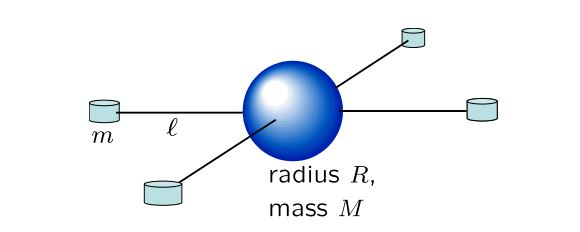
\includegraphics[width=0.7\textwidth]{f12.jpg}
\caption{四旋翼力矩图\ucite{4}}
\label{fig20}
\end{figure}
如图\ref{fig20}所示,四旋翼关于三个坐标轴几何对称性,因此${J_{xy}} = {J_{xz}} = {J_{yz}} = 0$,可得
\[J = \left( {\begin{array}{*{20}{c}}
{{J_x}}&0&0\\
0&{{J_y}}&0\\
0&0&{{J_z}}
\end{array}} \right)\]

因此,
\[{J^{ - 1}} = \left( {\begin{array}{*{20}{c}}
{\frac{1}{{{J_x}}}}&0&0\\
0&{\frac{1}{{{J_y}}}}&0\\
0&0&{\frac{1}{{{J_z}}}}
\end{array}} \right)\]

如图\ref{fig20}所示,球体的转动惯量为$J = \frac{2}{5}M{R^2}$,从而就可得到:
\[\begin{array}{l}
{J_x} = \frac{2}{5}M{R^2} + 2{l^2}m\\
{J_y} = \frac{2}{5}M{R^2} + 2{l^2}m\\
{J_z} = \frac{2}{5}M{R^2} + 4{l^2}m
\end{array}\]

定义力矩${m^b} \buildrel \Delta \over = {\left( {{\tau _\phi },{\tau _\theta },{\tau _\psi }} \right)^T}$,代入公式
(3.5)可得:
\[\begin{array}{l}
\left( \begin{array}{l}
\mathop p\limits^ \cdot  \\
\mathop q\limits^ \cdot  \\
\mathop r\limits^ \cdot
\end{array} \right) = \left( {\begin{array}{*{20}{c}}
{\frac{1}{{{J_x}}}}&0&0\\
0&{\frac{1}{{{J_y}}}}&0\\
0&0&{\frac{1}{{{J_z}}}}
\end{array}} \right)\left[ {\left( {\begin{array}{*{20}{c}}
0&r&{ - q}\\
{ - r}&0&p\\
q&{ - p}&0
\end{array}} \right)\left( {\begin{array}{*{20}{c}}
{{J_x}}&0&0\\
0&{{J_y}}&0\\
0&0&{{J_z}}
\end{array}} \right)\left( \begin{array}{l}
p\\
q\\
r
\end{array} \right) + \left( \begin{array}{l}
{\tau _\phi }\\
{\tau _\theta }\\
{\tau _\psi }
\end{array} \right)} \right]\\
{\kern 1pt} {\kern 1pt} {\kern 1pt} {\kern 1pt} {\kern 1pt} {\kern 1pt} {\kern 1pt} {\kern 1pt} {\kern 1pt} {\kern 1pt} {\kern 1pt} {\kern 1pt} {\kern 1pt} {\kern 1pt} {\kern 1pt} {\kern 1pt} {\kern 1pt} {\kern 1pt}  = \left( \begin{array}{l}
\frac{{{J_y} - {J_z}}}{{{J_x}}}qr\\
\frac{{{J_z} - {J_x}}}{{{J_y}}}pr\\
\frac{{{J_x} - {J_y}}}{{{J_z}}}pq
\end{array} \right) + \left( \begin{array}{l}
\frac{1}{{{J_x}}}{\tau _\phi }\\
\frac{1}{{{J_y}}}{\tau _\theta }\\
\frac{1}{{{J_z}}}{\tau _\psi }
\end{array} \right)\\
{\kern 1pt} {\kern 1pt} {\kern 1pt} {\kern 1pt} {\kern 1pt} {\kern 1pt} {\kern 1pt}
\end{array}\]

最后,六自由度飞行动力学方程如下所示。
\begin{equation}
\left( \begin{array}{c}
\mathop {{p_n}}\limits^ \cdot  \\
\mathop {{p_e}}\limits^ \cdot  \\
h
\end{array} \right) = \left( {\begin{array}{*{20}{c}}
{c\theta c\psi }&{s\phi s\theta c\psi  - c\phi s\psi }&{c\phi s\theta c\psi  + s\phi s\psi }\\
{c\theta s\psi }&{s\phi s\theta s\psi  + c\phi c\psi }&{c\phi s\theta s\psi  - s\phi c\psi }\\
{s\theta }&{ - s\phi c\theta }&{ - c\phi c\theta }
\end{array}} \right)\left( \begin{array}{l}
u\\
v\\
\omega
\end{array} \right)
\end{equation}
\begin{equation}
\left( \begin{array}{l}
\mathop u\limits^ \cdot  \\
\mathop v\limits^ \cdot  \\
\mathop \omega \limits^ \cdot
\end{array} \right) = \left( \begin{array}{l}
rv - q\omega \\
p\omega  - ru\\
qu - pv
\end{array} \right) + \frac{1}{m}\left( \begin{array}{l}
{f_x}\\
{f_y}\\
{f_z}
\end{array} \right)
\end{equation}
\begin{equation}
\left( \begin{array}{l}
\mathop \phi \limits^ \cdot  \\
\mathop \theta \limits^ \cdot  \\
\mathop \psi \limits^ \cdot
\end{array} \right) = \left( {\begin{array}{*{20}{c}}
1&{\sin \phi \tan \theta }&{\cos \phi \tan \theta }\\
0&{\cos \phi }&{ - \sin \phi }\\
0&{\frac{{\sin \phi }}{{\cos \theta }}}&{\frac{{\cos \phi }}{{\cos \theta }}}
\end{array}} \right)\left( \begin{array}{l}
p\\
q\\
r
\end{array} \right)
\end{equation}
\begin{equation}
\left( \begin{array}{l}
\mathop p\limits^ \cdot  \\
\mathop q\limits^ \cdot  \\
\mathop r\limits^ \cdot
\end{array} \right) = \left( \begin{array}{l}
\frac{{{J_y} - {J_z}}}{{{J_x}}}qr\\
\frac{{{J_z} - {J_x}}}{{{J_y}}}pr\\
\frac{{{J_x} - {J_y}}}{{{J_z}}}pq
\end{array} \right) + \left( \begin{array}{l}
\frac{1}{{{J_x}}}{\tau _\phi }\\
\frac{1}{{{J_y}}}{\tau _\theta }\\
\frac{1}{{{J_z}}}{\tau _\psi }
\end{array} \right)
\end{equation}

\subsubsection{四旋翼力和力矩方程}
对于四旋翼而言,因为没有空气动力学的升力面,所以,四旋翼的气动力和气动力矩是可以忽略的。四旋翼的力和力矩主要来自于重力和四个螺旋桨的推力。如图\ref{fig21}所示。
\vspace{-20pt}
\begin{figure}[!ht]
\centering
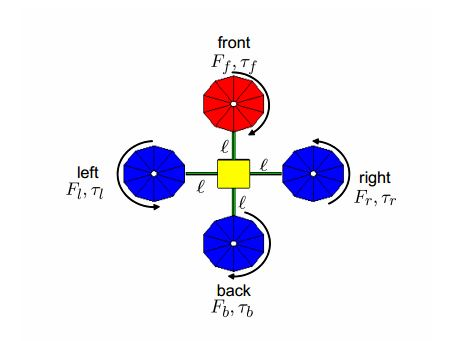
\includegraphics[width=0.7\textwidth]{f13.jpg}
\caption{四旋翼力和力矩俯视图\ucite{4}}
\label{fig21}
\end{figure}

\begin{figure}[!ht]
\centering
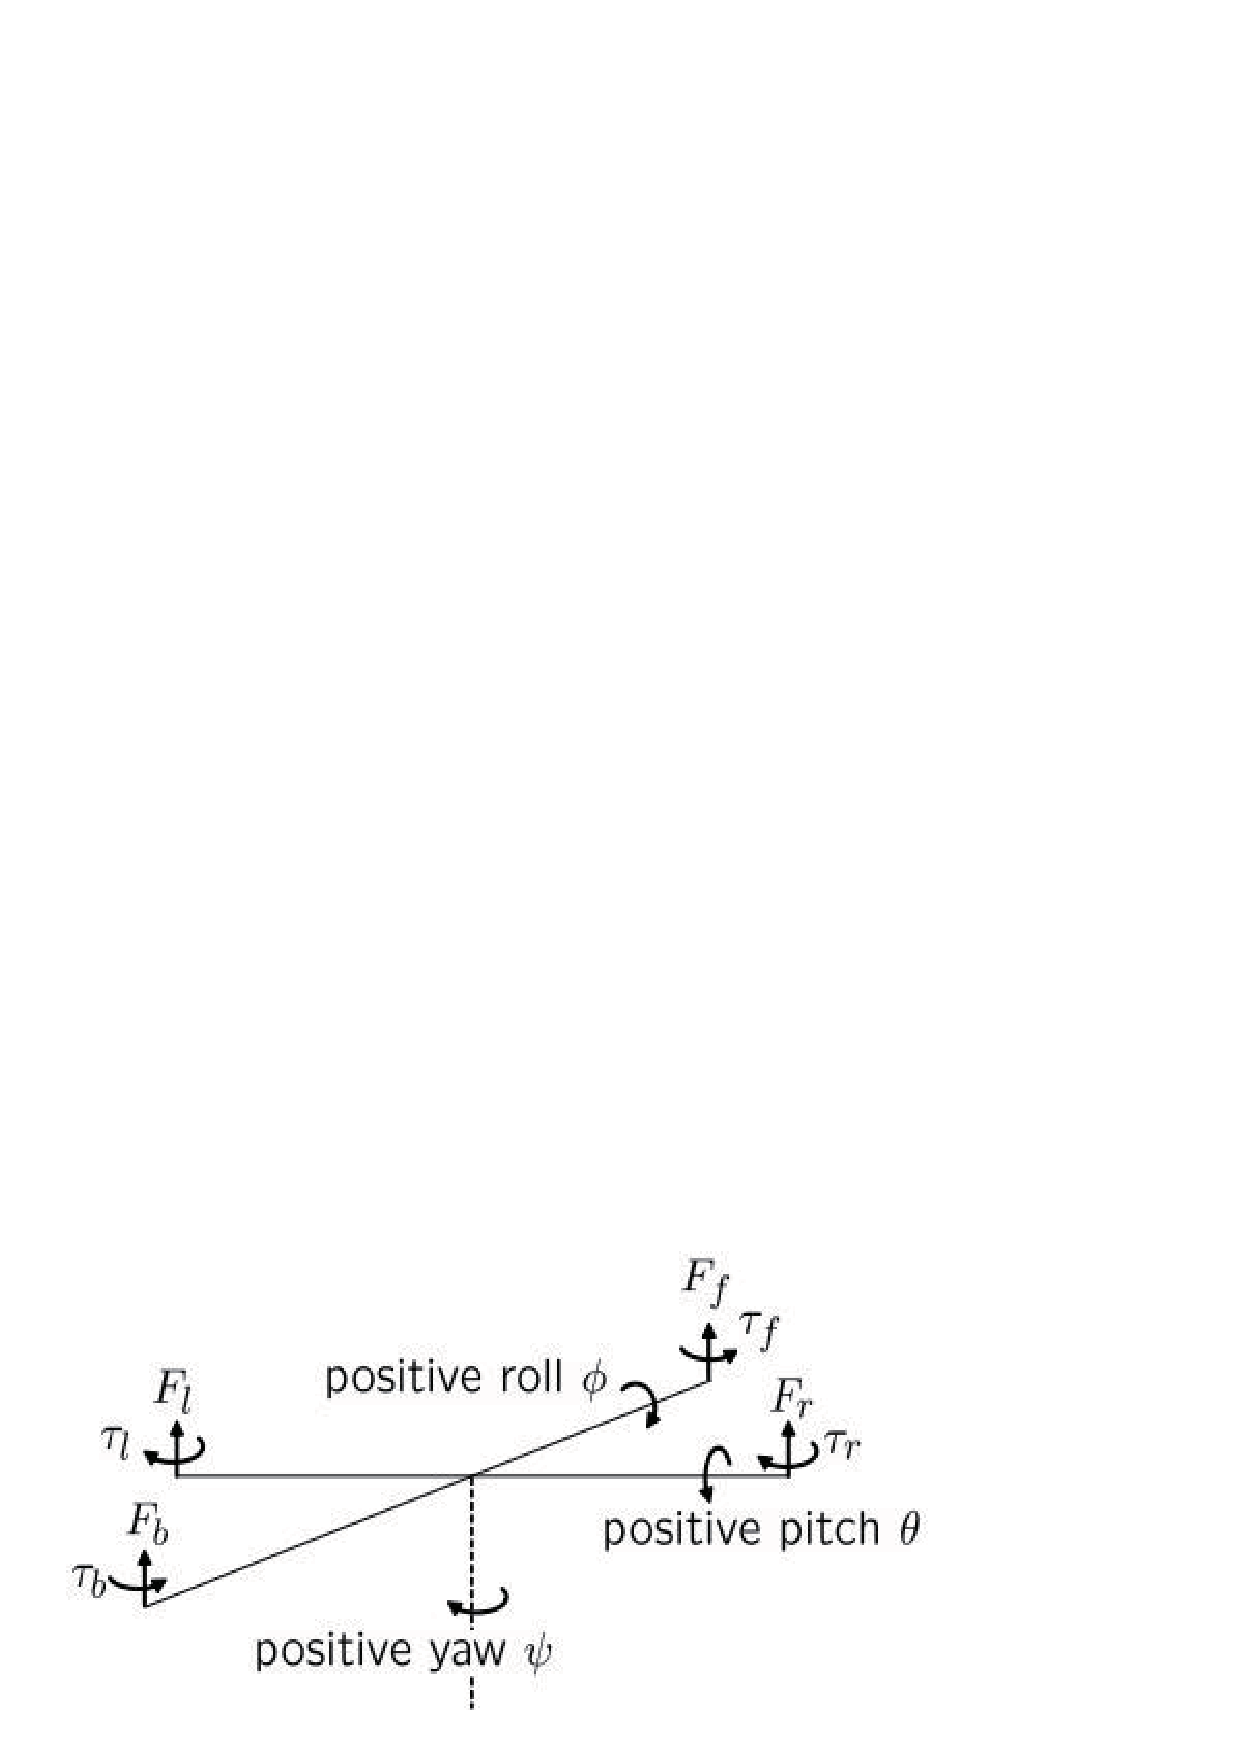
\includegraphics[width=0.7\textwidth]{f14.jpg}
\caption{四旋翼力和力矩俯视图\ucite{4}}
\label{fig22}
\end{figure}
由图\ref{fig21}所示,是从四旋翼的俯视图来得到的力和力矩图。图\ref{fig22}所示的四旋翼力和力矩的受力简化图,每个螺旋剑电机产生力和力矩。作用于四旋翼上的力可以表示为:
\[F = {F_f} + {F_r} + {F_b} + {F_l}\]

如图\ref{fig22}所示,左右电机产生的滚转力矩可以表示为:
\[{\tau _\phi } = l\left( {{F_l} - {F_r}} \right)\]

同理,前后电机产生的俯仰力矩可以表示为:
\[{\tau _\theta } = l\left( {{F_f} - {F_b}} \right)\]

由牛顿第三定律可知,阻力产生的偏航力矩反作用于四旋翼,方向与四旋翼的旋转方向相反。因此,四旋翼的旋转矩阵可以表示为:
\[{\tau _\psi } = {\tau _r} + {\tau _l} - {\tau _f} - {\tau _b}\]

由螺旋桨产生的升力和阻力,与角速度的平方成线性关系,如下所示:
\[\begin{array}{l}
{F_ * }{\rm{  = }}{k_1}{\delta _ * }\\
{\tau _ * } = {k_2}{\delta _ * }
\end{array}\]

其中,系数${k_1}$和${k_2}$由实验可以测得,${\delta _ * }$电机控制的信号,$ * $表示$f$,$r$,$b$,$l$电机。作用在四旋翼上力和力矩的矩阵如下所示:
\[\left( \begin{array}{l}
F\\
{\tau _\phi }\\
{\tau _\theta }\\
{\tau _\psi }
\end{array} \right) = \left( {\begin{array}{*{20}{c}}
{{k_1}}&{{k_1}}&{{k_1}}&{{k_1}}\\
0&{ - l{k_1}}&0&{l{k_1}}\\
{l{k_1}}&0&{l{k_1}}&0\\
{ - {k_2}}&{{k_2}}&{ - {k_2}}&{{k_2}}
\end{array}} \right)\left( \begin{array}{l}
{\delta _f}\\
{\delta _r}\\
{\delta _b}\\
{\delta _l}
\end{array} \right) \buildrel \Delta \over = M\left( \begin{array}{l}
{\delta _f}\\
{\delta _r}\\
{\delta _b}\\
{\delta _l}
\end{array} \right)\]

四旋翼除了受电机产生的作用力外,还有自身的重力,在速度坐标系$\mathop R\nolimits^v $下,重力恰好作用与坐标系的重心位置,故:
\[\mathop f\nolimits_g^v  = \left( \begin{array}{c}
0\\
0\\
mg
\end{array} \right)\]

但是,速度是在机体坐标系下表示的,故上式需转换在机体坐标系下:
\[\begin{array}{l}
\mathop f\nolimits_g^b  = \mathop R\nolimits_v^b \left( \begin{array}{c}
0\\
0\\
mg
\end{array} \right)\\
{\kern 1pt} {\kern 1pt} {\kern 1pt} {\kern 1pt} {\kern 1pt} {\kern 1pt} {\kern 1pt} {\kern 1pt} {\kern 1pt} {\kern 1pt} {\kern 1pt} {\kern 1pt} {\kern 1pt} {\kern 1pt} {\kern 1pt} {\kern 1pt} {\kern 1pt} {\kern 1pt} {\kern 1pt}  = \left( \begin{array}{l}
 - mg\sin \theta \\
mg\cos \theta \sin \phi \\
mg\cos \theta \cos \phi
\end{array} \right)
\end{array}\]

最终,四旋翼的六自由度飞行动力学模型如下:
\begin{equation}
\left( \begin{array}{c}
\mathop {{p_n}}\limits^ \cdot  \\
\mathop {{p_e}}\limits^ \cdot  \\
h
\end{array} \right) = \left( {\begin{array}{*{20}{c}}
{c\theta c\psi }&{s\phi s\theta c\psi  - c\phi s\psi }&{c\phi s\theta c\psi  + s\phi s\psi }\\
{c\theta s\psi }&{s\phi s\theta s\psi  + c\phi c\psi }&{c\phi s\theta s\psi  - s\phi c\psi }\\
{s\theta }&{ - s\phi c\theta }&{ - c\phi c\theta }
\end{array}} \right)\left( \begin{array}{l}
u\\
v\\
\omega
\end{array} \right)
\end{equation}
\begin{equation}
\left( \begin{array}{l}
\mathop u\limits^ \cdot  \\
\mathop v\limits^ \cdot  \\
\mathop \omega \limits^ \cdot
\end{array} \right) = \left( \begin{array}{l}
rv - q\omega \\
p\omega  - ru\\
qu - pv
\end{array} \right) + \left( \begin{array}{c}
 - g\sin \theta \\
g\cos \theta \sin \phi \\
g\cos \theta \cos \phi
\end{array} \right) + \frac{1}{m}\left( \begin{array}{c}
0\\
0\\
 - F
\end{array} \right)
\end{equation}
\begin{equation}
\left( \begin{array}{l}
\mathop \phi \limits^ \cdot  \\
\mathop \theta \limits^ \cdot  \\
\mathop \psi \limits^ \cdot
\end{array} \right) = \left( {\begin{array}{*{20}{c}}
1&{\sin \phi \tan \theta }&{\cos \phi \tan \theta }\\
0&{\cos \phi }&{ - \sin \phi }\\
0&{\frac{{\sin \phi }}{{\cos \theta }}}&{\frac{{\cos \phi }}{{\cos \theta }}}
\end{array}} \right)\left( \begin{array}{l}
p\\
q\\
r
\end{array} \right)
\end{equation}
\begin{equation}
\left( \begin{array}{l}
\mathop p\limits^ \cdot  \\
\mathop q\limits^ \cdot  \\
\mathop r\limits^ \cdot
\end{array} \right) = \left( \begin{array}{l}
\frac{{{J_y} - {J_z}}}{{{J_x}}}qr\\
\frac{{{J_z} - {J_x}}}{{{J_y}}}pr\\
\frac{{{J_x} - {J_y}}}{{{J_z}}}pq
\end{array} \right) + \left( \begin{array}{l}
\frac{1}{{{J_x}}}{\tau _\phi }\\
\frac{1}{{{J_y}}}{\tau _\theta }\\
\frac{1}{{{J_z}}}{\tau _\psi }
\end{array} \right)
\end{equation}

\subsection{模型求解}

六自由度的四旋翼飞行动力学方程太复杂对于模型求解而言。本文基于小扰动假设,即果运动参数偏离基准状态的量为小量,可以略去二阶以上的运动参数变化量。在线性化的过程中,可以把无人机运动近似的分解为纵向运动和横向运动,两种运动相互独立。纵向运动即是飞机的俯仰运动;横向运动对应的是飞机的偏航与滚转运动。

假设$\phi$和$\theta$都是小量可以忽略,故公式(3.12)可以简化为:
\[\left( \begin{array}{l}
\mathop \phi \limits^ \cdot  \\
\mathop \theta \limits^ \cdot  \\
\mathop \psi \limits^ \cdot
\end{array} \right) = \left( \begin{array}{l}
p\\
q\\
r
\end{array} \right)\]

同理,假设Coriolis方程中$qr$,$pr$,$pq$均为小量可以忽略,故公式(3.13)可以简化为:
\[\left( \begin{array}{l}
\mathop p\limits^ \cdot  \\
\mathop q\limits^ \cdot  \\
\mathop r\limits^ \cdot
\end{array} \right) = \left( \begin{array}{l}
\frac{1}{{{J_x}}}{\tau _\phi }\\
\frac{1}{{{J_y}}}{\tau _\theta }\\
\frac{1}{{{J_z}}}{\tau _\psi }
\end{array} \right)\]

结合上面两式,可得:
\begin{equation}
\left( \begin{array}{l}
\mathop \phi \limits^{ \cdot  \cdot } \\
\mathop \theta \limits^{ \cdot  \cdot } \\
\mathop \psi \limits^{ \cdot  \cdot }
\end{array} \right) = \left( \begin{array}{l}
\frac{1}{{{J_x}}}{\tau _\phi }\\
\frac{1}{{{J_y}}}{\tau _\theta }\\
\frac{1}{{{J_z}}}{\tau _\psi }
\end{array} \right)
\end{equation}

对公式(3.10)求微分可得:
\[\left( {\begin{array}{*{20}{c}}
{c\theta c\psi }&{s\phi s\theta c\psi  - c\phi s\psi }&{c\phi s\theta c\psi  + s\phi c\psi }\\
{c\theta s\psi }&{s\phi s\theta s\psi  + c\phi c\psi }&{c\phi s\theta s\psi  - s\phi c\psi }\\
{ - s\theta }&{s\phi c\theta }&{c\phi c\theta }
\end{array}} \right)\]

对公式(3.11)忽略Coriolis量,代入上式可得:
\[\left( \begin{array}{l}
\mathop {{p_n}}\limits^{ \cdot  \cdot } \\
\mathop {{p_e}}\limits^{ \cdot  \cdot } \\
\mathop {{p_d}}\limits^{ \cdot  \cdot }
\end{array} \right) = \left( \begin{array}{l}
0\\
0\\
g
\end{array} \right) + \left( \begin{array}{c}
 - c\phi s\theta c\psi  - s\phi s\psi \\
 - c\phi s\theta s\psi  + s\phi c\psi \\
 - c\phi c\theta
\end{array} \right)\frac{F}{m}\]

因此,在惯性坐标系下,简化的方程如下:
\begin{equation}
\mathop {{p_n}}\limits^{ \cdot  \cdot }  = \left( { - \cos \phi \sin \theta \cos \psi  - \sin \phi \sin \psi } \right)\frac{F}{m}
\end{equation}
\begin{equation}
\mathop {{p_e}}\limits^{ \cdot  \cdot }  = \left( { - \cos \phi \sin \theta sin\psi  + \sin \phi \cos \psi } \right)\frac{F}{m}
\end{equation}
\begin{equation}
\mathop {{p_d}}\limits^{ \cdot  \cdot }  = g - \left( {\cos \phi \cos \theta } \right)\frac{F}{m}
\end{equation}
\begin{equation}
\mathop \phi \limits^{ \cdot  \cdot }  = \frac{1}{{{J_x}}}{\tau _\phi }
\end{equation}
\begin{equation}
\mathop \theta \limits^{ \cdot  \cdot }  = \frac{1}{{{J_y}}}{\tau _\theta }
\end{equation}
\begin{equation}
\mathop \psi \limits^{ \cdot  \cdot }  = \frac{1}{{{J_z}}}{\tau _\psi }
\end{equation}

\section{三维视景系统}\label{3}

三维可视仿真系统的结构如图 \ref{fig23}所示,主要包括仿真模块、飞行数据模块、通信模块、飞机模型库、纹理材质库等。
\vspace{-10pt}
\begin{figure}[!ht]
\centering
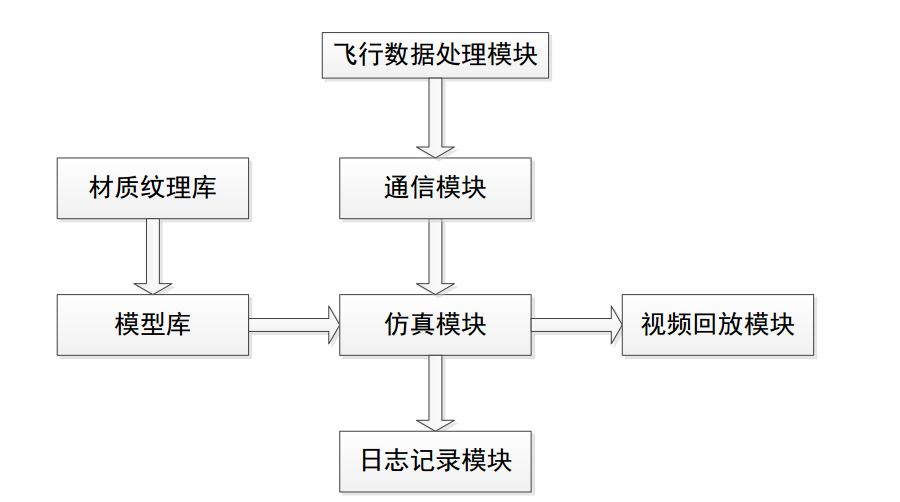
\includegraphics[width=0.7\textwidth]{f21.jpg}
\caption{三维可视化仿真结构图\ucite{16}}
\label{fig23}
\end{figure}

仿真模块是三维可视仿真系统的核心模块。一般使用高级程序语言(如 C++)编写,也可以调用第三方三维可视仿真软件实现。仿真模块主要完成以下功能\ucite{17}:
\begin{itemize}
  \item  接收通信模块传来的飞行数据。
  \item  从模型库中导入飞行器模型、场景模型、声音模型,并对飞行器进行姿态和位置调整。
  \item 驱动飞行器模型按照飞行数据在场景中进行模拟飞行。
\end{itemize}

模型库为仿真系统提供飞行模型,包括飞行器模型、场景模型、建筑物模型、声音模型等,其中飞行器模型最为重要。并从材质纹理库读取纹理介质,将纹理介质贴于飞行器或场景表面,使模型更加美观、逼真\ucite{yuyanping2010}。

材质纹理库为模型库中的各种模型的表面提供纹理介质,主要起美化作用。

飞行数据模块中的数据可以来自实时的飞行数据,也可以来自飞行动力学模型的模拟数据(如使用 matlab/simlink 构建动力学模型进行模拟),或者离线的外部数据\ucite{18}。

通信模块负责飞行数据模块与仿真模块之间的通信,一般使用 socket 编程实现,飞行数据模块作为客户端,仿真模块作为服务端。在数据链路层还可以使用循环冗余校验码对飞行数据进行检验\ucite{19}。

日志记录/回放模块用来记录模拟飞行时飞行器的位置和姿态信息,进行仿真过程回放,以便对某次或者某段仿真结果进行分析,查找可能存在的问题\ucite{20}。







\chapter{固定翼无人机飞控建模}\label{routing}
本文进行固定翼无人机飞控建模,选择c172p飞机。固定翼飞机与四旋翼飞机在空气动力学特性等方面存在着很多不同。本文采用FlightGear自带的JSBSim飞行动力学模型,进行固定翼飞机的飞行控制,如图\ref{fig40}所示。
\vspace{-10pt}
\begin{figure}[!ht]
\centering
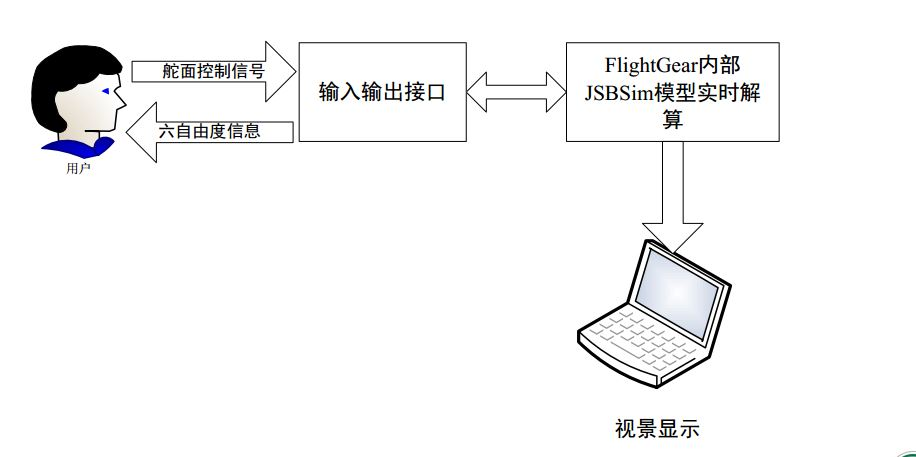
\includegraphics[width=0.8\textwidth]{f33.jpg}
\caption{固定翼飞控建模过程}
\label{fig40}
\end{figure}
\vspace{-10pt}
\section{JSBSim介绍}
JSBsim 是一个通用的 6 自由度动态模型,模拟飞行工具的运动。它使用 C++语言编写,可以运行在单机方式下,也可以驱动有视觉子系统的大型程序。YAsim是由 Andrew Ross 开发的新动力学模型,是 Flightgear 的集成部分,它通过模拟飞行器不同部分的气流来实现,这点不同于 JSBsim。UIUC 飞行动态模型是基于LaRCsim 的,最初是 NASA 开发的,通过使用飞行器配置文件来扩充代码\ucite{28}。目前 JSBsim\ucite{29}和 UIUC 是比较流行的动力学仿真系统,并且均是开源项目。

\section{JSBSim飞行动力学模型}
根据FlightGear自带的JSBSim飞行控制模型,进行飞行控制。包括飞机舵面的控制,飞机姿态的控制。
\begin{itemize}
  \item 升降舵控制

  升降舵主要控制飞机的俯仰姿态运动,在JSBSim中对升降舵控制的代码如下:
   \begin{lstlisting}[language==XML]
<flight_control name="FCS:c172p">
<channel name="All">
    <summer name="Pitch Trim Sum">
        <input>fcs/elevator-cmd-norm</input>
        <input>fcs/pitch-trim-cmd-norm</input>
        <clipto>
            <min>-1</min>
            <max>1</max>
        </clipto>
</summer>
<aerosurface_scale name="Elevator Control">
    <input>fcs/pitch-trim-sum</input>
        <range>
            <min>-0.35</min>
            <max>0.3</max>
        </range>
    <output>fcs/elevator-pos-rad</output>
</aerosurface_scale>
 \end{lstlisting}
  \item 方向舵控制

  方向舵主要控制飞机的偏航运动,在小飞机转弯的过程中,起着重要的作用。JSBSim的代码如下:
  \begin{lstlisting}[language==XML]
<summer name="Rudder Command Sum">
    <input>fcs/rudder-cmd-norm</input> 
    <input>fcs/yaw-trim-cmd-norm</input>
    <clipto>
        min>-1</min>
        <max>1</max>
    </clipto>
</summer>
<aerosurface_scale name="Rudder Control">
    <input>fcs/rudder-command-sum</input>
        <range>
            <min>-0.35</min>
            <max>0.35</max>
        </range>
    <output>fcs/rudder-pos-rad</output>
</aerosurface_scale>
 \end{lstlisting}
  \item 副翼控制
  
  副翼主要控制飞机的滚转运动,副翼分为左右副翼,JSBSim控制代码如下:
    \begin{lstlisting}[language==XML]
<summer name="Roll Trim Sum">
    <input>fcs/aileron-cmd-norm</input>
    <input>fcs/roll-trim-cmd-norm</input>
        <clipto>
            <min>-1</min>
            <max>1</max>
        </clipto>
</summer>
<aerosurface_scale name="Left Aileron Control">
    <input>fcs/roll-trim-sum</input>
        <range>
            <min>-0.35</min>
            <max>0.35</max>
        </range>
    <output>fcs/left-aileron-pos-rad</output>
</aerosurface_scale>
<aerosurface_scale name="Right Aileron Control">
    <input>-fcs/roll-trim-sum</input>
        <range>
            <min>-0.35</min>
            <max>0.35</max>
        </range>
    <output>fcs/right-aileron-pos-rad</output>
</aerosurface_scale>
 \end{lstlisting}
\end{itemize}

本文选择c172p飞机,如图\ref{fig41}所示,结合上面JSBsim模型对c172p进行飞行控制。

\begin{figure}[!ht]
\centering
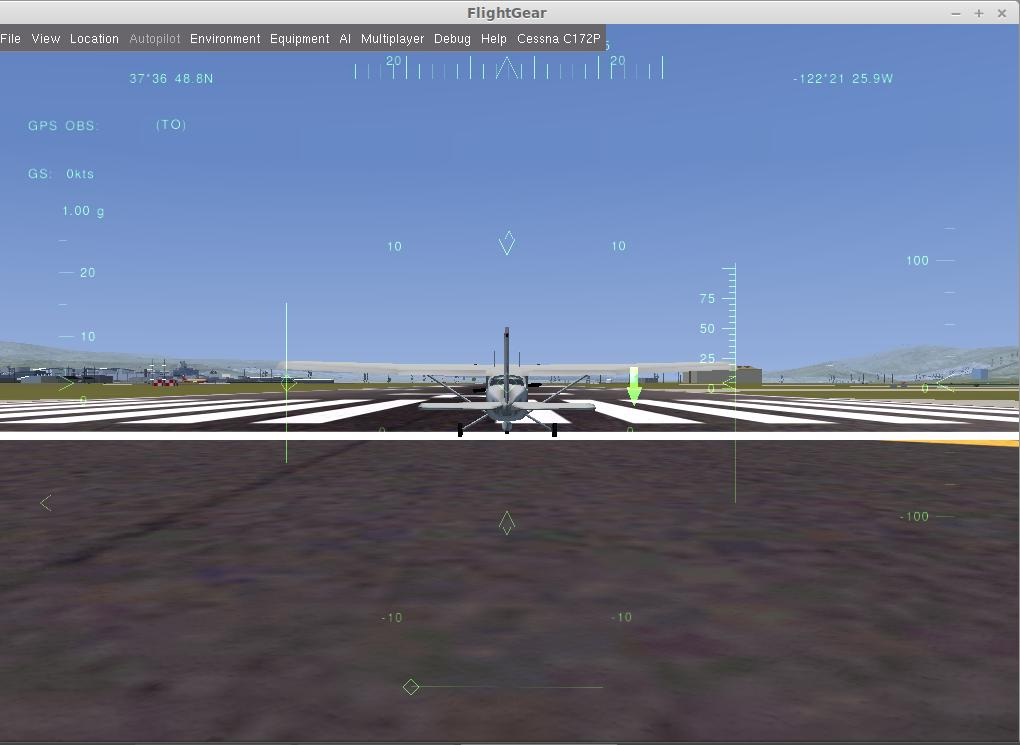
\includegraphics[width=0.6\textwidth]{f34.jpg}
\caption{固定翼飞控建模过程}
\label{fig41}
\end{figure}



\chapter{FlightGear仿真效果}\label{forward}

本章主要介绍FLightGear仿真效果,首先,是介绍FlightGear驱动飞行器模拟的步骤;然后,是介绍FlightGear系统实施的软硬件环境;最后,是展示四旋翼飞行仿真效果。
\section{FlightGear飞行模拟器驱动}
FlightGear实现对飞行模拟器的驱动,需要经过飞行模拟器载入及配置的过程,然后,需要设置FlightGear通信模块,最后,进行飞行数据的处理。  FlightGear使用xml文件对模型进行配置,包括飞行器的位置,动作及姿态\ucite{21}。
\begin{enumerate}
  \item  载入飞行器模型,主要是通过-set.xml 文件指定使用的飞行器模型、场景模型和声音模型等;
  \item  根据载入效果,通过配置文件调整飞行器位置及姿态;
  \item  配置飞行器需要完成的动作,对于四旋翼无人机来说,主要是螺旋桨的旋转。
\end{enumerate}

\subsection{飞行模拟器载入及配置}
基于FlightGear良好的三维图像兼容特性,可以方便导入三维飞行器模型。在FlightGear中
FlightGear 飞行模型的主配置文件是 XML 类型文件,命名规则为“飞行器模型名-set.xml”,因此每个飞行器模型都必须有一个独一无二的名字,本系统中的四旋翼无人机模型命名为 Quarotor,主配置文件命名为 quarotor-set.xml,该配置文件主要完成以下配置:
\begin{enumerate}
\item
  指定飞行器模型\ucite{23}

  使用/sim/model/path参数指定飞行器模型的配置文件,该配置文件也是XML格式,一般习惯以飞行器模型的名称直接命名,但不是必须的。相关配置语句如下:
 \begin{lstlisting}[language={[ANSI]C++}]
<sim>
  <model>
   <path>Aircraft/arducopter/Models/arducopter.xml</path>
  </model>
</sim>
\end{lstlisting}
quadrotor.xml 指定用到的飞行器模型,如本系统使用的四旋翼无人机模型quadrotor.ac 文件,该文件与 quadrotor.xml 位于同一目录下。quadrotor.xml 最主要的作用其实是配置飞行器模型需要完成的各项动作,相关配置语句如下:
\begin{lstlisting}[language={[ANSI]C++}]
<PropertyList>
   <path>quadrotor.ac</path>
</PropertyList>
\end{lstlisting}
\item 指定声音模型\ucite{23}

使用/sim/sound/path 参数指定仿真飞行时使用的声音配置文件,四旋翼无人机飞行声音主要是螺旋桨旋转的轰鸣声、风声,没有特殊声音,可以使用FlightGear 提供的基本声音配置文件,具体配置代码如下:
\begin{lstlisting}[language={[ANSI]C++}]
<sound>
      <path>Aircraft/Generic/generic-sound.xml</path>
</sound>
\end{lstlisting}

\item 指定飞行动力学模型\ucite{23}

本系统使用 FlightGear 进行虚拟现实的显示,飞行器模型的飞行通过动力学模型控制。动力学系统通过解算动力学模型,将飞行模型的姿态和位置等信息参数通过通信模块发送到飞行控制系统,飞行控制系统将信息参数转换成控制命令传递到 FlightGear 进行视景更新。

使用哪种飞行动力学模型可以使用两种方式进行指定,一种仍然是通过主配置文件,使用/sim/flight-model 参数,比如指定使用 JSBsim 动力学模型的代码如下:
\begin{lstlisting}[language={[ANSI]C++}]
<sim>
    <flight-model>jsb</flight-model>
</sim>
\end{lstlisting}
另一种方法是在启动 FlightGear 时直接使用命令行参数指定,格式如“--fdm=jsb”。除了可以选用 FlightGear 提供的动力学模型,FlightGear 也支持用户自己编写动力学模型,此时使用“--fdm=external”命令,此命令通知FlightGear 接受外部数据。
\item 指定飞行器动作参数

为了增加仿真效果的逼真度,飞行器的某些部位应该能完成相应的动作,如螺旋桨旋转、起落架的放下/收起、驾驶舱门的开启/关闭、风向舵的偏转等。这些动作的完成都需要配置相关的动作参数。四旋翼无人机的主要动作是四个螺旋桨的旋转,需要配置螺旋桨的转速,配置代码如下:
\begin{lstlisting}[language={[ANSI]C++}]
<engines>
<engine>
   <rpm type="double">350</rpm>
</engine>
</engines>
\end{lstlisting}
代码中 rpm 代表每分钟旋转的次数,其值被设置为 350,类型为 double(双精度数字)。此配置方法在使用“--fdm=external”命令时无效,此时如果需要使用 rpm 参数则需要在 FlightGear 通信模型中设置相应变量。

飞行器模型的动作需要使用此参数时,使用“/engines/engine[0]/rpm”字符串,具体配置方式如下:
\begin{lstlisting}[language={[ANSI]C++}]
<property>/engines/engine[0]/rpm</property>
\end{lstlisting}
\end{enumerate}
\subsection{飞行器模型的动作}
飞行器模型需要在仿真飞行时完成一定的动作,如螺旋桨旋转。FlightGear允许用户控制飞行器的任意部位完成相应的工作,唯一要求就是这一部位在三维模型中被命名过,即设置了对象名称(object name)。

FlightGear 现在主要支持以下几种类型的动作:none、billboard、rotate、scale、blend、select、spin、timed、translate、texrotate、textranslate、textmultiple、material、
range、alpha-test、noshadow。四旋翼无人机模型主要用的了 noshadow、select、spin、spin 四种类型。下面以其中一个旋翼的动作为例结合实际代码介绍这四种动作类型的含义及用法,其他三个旋翼与之类似:
\begin{itemize}
  \item Noshadow:

无阴影动作类型,使该对象屏蔽投射阴影的命令,如螺旋桨的阴影本身已经是阴影,不能再投射出阴影。具体用法:使用 type 标签指定动作类型 noshadow,使用 object-name 标签指定该动作的作用对象,该标签的属性值必须与三维模型中设置的对象名称完全一致。具体代码如下:
\begin{lstlisting}[language={[ANSI]C++}]
<animation>
  <type>noshadow</type>
  <object-name>Propeller1.Spinning</object-name>
</animation>
\end{lstlisting}
  \item Select

选择动作类型,根据配置的条件决定选择哪个对象显示。当螺旋桨转速低于一定值的时候显示螺旋桨,当转速高于一定值后显示螺旋桨阴影,用于无人机启动或熄火时制造螺旋桨加速、减速的效果。property 标签的属性值必须是 quarotor-set.xml 主配置文件配置过的动作参数,具体代码如下:
\begin{lstlisting}[language=XML]
<animation>
 <type>select</type>
  <object-name>Propeller1</object-name>
   <condition>
     <less-than>
       <property>/engines/engine[0]/rpm</property>
       <value>350</value>
     </less-than>
   </condition>
</animation>
\end{lstlisting}
  \item Spin

旋转动作类型,是无人机模型最主要的动作类型,其控制螺旋桨旋转中心、旋转轴。property 标签指定转速,center 标签指定旋转中心,axis 标签指定旋转轴。旋转中心使用的坐标系为机体坐标系,具体坐标应是三维无人机模型中的实际坐标,具体代码如下:
 \begin{lstlisting}
 <animation>
    <type>spin</type>
    <object-name>propeller0</object-name>
    <property>/controls/engines/engine[0]/throttle</property>
    <factor>12000</factor>
    <axis>
      <x1-m>0.000</x1-m>
      <y1-m>-0.288</y1-m>
      <z1-m>0.046</z1-m>
      <x2-m>0.000</x2-m>
      <y2-m>-0.288</y2-m>
      <z2-m>0.012</z2-m>
    </axis>
  </animation>
 \end{lstlisting}
\end{itemize}


\subsection{通信模块}
在飞行器模型载入 FlightGear 并完成相应的配置之后,下一步就是驱动飞行器模型进行仿真了。本节将介绍 FlightGear 使用的通信模型,并主要介绍如何实现外部模拟数据与 FlightGear 进行通信来驱动飞行器模型。

\begin{enumerate}
  \item  FlightGear 通信模型

本文说的通信模型指的是通信双方都认可的通信格式\ucite{21}。要与 FlightGear通信,必须使用 FlightGear 的通信模型FlightGear 的通信模型为了保证通用性,包含了飞行器模型飞行时需要的所有参数信息。本文在进行四旋翼无人机的三维可视仿真时只用到部分参数,主要参数如表\ref{t1}所示。
\newpage
\begin{table}[!h]\label{t1}
\begin{center}
\caption{四旋翼无人机飞行需要的主要参数}\label{t1}
\begin{longtable}{ | c| c|}
\hline
参数名称                                    & 参数意义                                                                  \\\hline
FG\_NET\_FDM\_VERSION                     & 通信模型版本号,同一版本的通信模型才能通信
                               \\\hline
longitude           & 经度,单位是度
                                   \\\hline
latitude              & 纬度,单位是度
                                            \\\hline
altitude                     & 海拔,单位是英尺

                                          \\\hline
$\phi $             & 滚转角,从后向前视角的顺时针旋转为正。
\\\hline
$\theta $ &俯仰角,从左向右视角的顺时针旋转为正。
\\\hline
$\psi $  &  偏航角,从上向下视角的顺时针旋转为正。
\\\hline
eng\_state  &   发动机状态(0:关闭,1:启动,2:运行)
\\\hline
rpm &  螺旋桨转速
\\\hline
\end{longtable}
\end{center}
\end{table}
\vspace{-40pt}
 \item 通信模块的实现

通信模块用于连接飞行数据模块和仿真模块,完成数据的接收和发送,如图\ref{fig24}。驱动飞行器模型进行仿真的方式主要有动力学模型驱动、外部仿真数据驱动、真实飞行器的实时数据驱动。不管使用哪种方式,都涉及到如何与FlightGear进行通信,但是如果每一种驱动方式都编写各自的通信模型,肯定不是明智的选择。本文将基于Socket(套接字)为不同的驱动方式编写统一接口,实现对通信方式的模块化封装,使系统能够灵活的更换驱动方式。
\vspace{-10pt}
\begin{figure}[!ht]
\centering
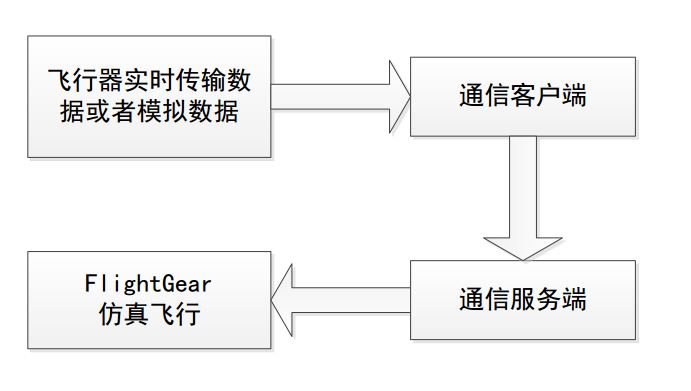
\includegraphics[width=0.6\textwidth]{f22.jpg}
\caption{通信模块的作用}
\label{fig24}
\end{figure}

为了实现在网络中传输数据,必须使用网络通信协议。TIP/IP协议是当前计算机网络中使用最多的网络通信协议,TCP/IP 的核心部分由网络操作系统的内核实现,应用程序通过编程接口来访问TCP/IP\ucite{22}。Socket是介于网络应用层和传输层之间的编程接口,套接字接口提供了访问下层通信协议的大量系统调用函数和相应的数据结构\ucite{23},Socket在通信协议中的地位\ref{fig25}所示。
\begin{figure}[!ht]
\centering
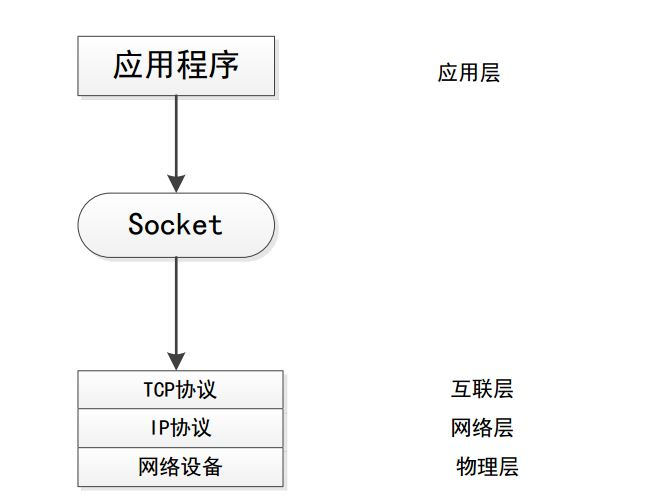
\includegraphics[width=0.6\textwidth]{f23.jpg}
\caption{Socket套接字在TCP/IP通信模型中的地位}
\label{fig25}
\end{figure}

TCP/IP协议的体系结构如图\ref{fig26}所示\ucite{24},其中网络层有两种通信协议TCP和UDP:
 \begin{figure}[!ht]
\centering
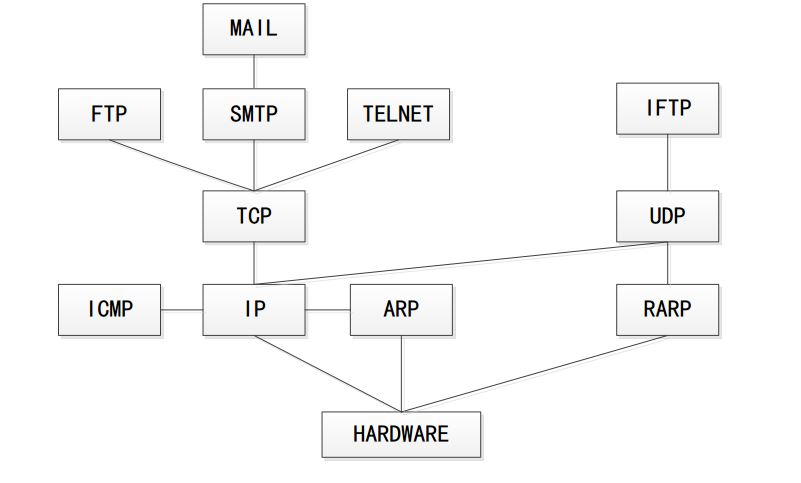
\includegraphics[width=0.6\textwidth]{f24.jpg}
\caption{TCP/IP协议框架}
\label{fig26}
\end{figure}

FlightGear支持使用TCP和UDP两种传输协议进行通信,出于以下几点考虑,本文使用基于数据报套接字的UDP协议开发通信模块:
\begin{itemize}
  \item 行模拟对实时性要求较高,UDP方式不用建立连接通道,不对数据进行校验,传输速率较快,能最大程度的保证飞行模拟的实时性;
  \item 飞行模拟在画面渲染和模拟数据的传输方面对系统资源的开销都很大,UDP方式没有TCP方式对数据质量的控制功能,能降低系统对硬件的要求,最大程度的保证仿真效果;
  \item 飞行模拟对数据的可靠行要求不是非常高,由于前后帧的模拟数据相差很小,丢失一帧甚至几帧的数据不会对模拟结果产生较大影响,因此虽然UDP方式不保证数据无差错,但是使用UDP方式的差错率是可以容忍的。

\end{itemize}

通信模块分为客户端和服务器端,客户端和服务器端可以部署于同一台机器,也可以部署到不同的机器上。在网络中进行通信至少需要一对套接字,其中一个运行于客户端,称之为ClientSocket;另一个运行于服务器端,称之为ServerSocket\ucite{26,27}。本系统使用UDP传输协议实现数据传输的流程图\ref{fig27}。
 \begin{figure}[!ht]
\centering
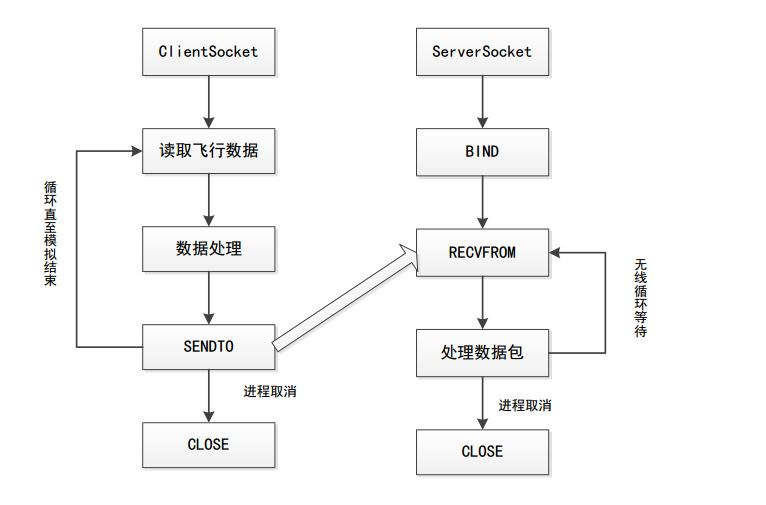
\includegraphics[width=0.8\textwidth]{f25.jpg}
\caption{UDP协议下的客户端与服务端通信流程}
\label{fig27}
\end{figure}
\end{enumerate}
服务器端进程依次进行如下操作:
\begin{itemize}
  \item 调用socket()方法创建一个数据报套接字(SOCK\_DGRAM);
  \item 调用bind()方法将服务器地址绑定在该套接字上;
  \item 调用recvfrom()方法等待客户端发来的数据包,此时程序进入无限循环
等待状态;
  \item 接受客户端传来的数据包,使用该数据包驱动飞行器模型完成相应的
动作;
  \item 继续等待接受客户端的请求;
  \item 服务器端关闭,注销该套接字。
\end{itemize}
客户进程依次进行如下操作:
\begin{itemize}
  \item 调用socket()方法创建一个数据报套接字(SOCK\_DGRAM);
  \item 读取飞行数据,并根据服务器地址向服务器端发送数据报;

数据来源可以是飞行器的实时飞行、动力学模型仿真,也可以是离线的外部数据,或者是FlightGear本身的日志记录文件。本文使用离线外部数据来测试三维可视仿真系统。以C++文件流方式读取外部文件,外部文件来源于joystick的数据读入部分。
\item 数据处理。数据处理主要包括度量单位转换(如弧度与角度转换)、坐标系转换。FlightGear使用测地学坐标系,如果外部数据是基于直角坐标系,则需要进行坐标转换。
\item 继续发送下一条飞行数据;

统通过基于UDP协议的Socket套接字进行发送,发送时间间隔有两种:

一种是指定固定时间间隔进行发送,如20毫秒,即每隔20毫秒发送1次数据,发送时间间隔是固定的;

另一种是根据外部数据的实际生成时间发送,即发送时间间隔不一定是固定的,此方式适合于非匀速变化。
\item 模拟仿真结束,注销该套接字。
\end{itemize}
\section{FlightGear仿真实现}
本节在前面几节的基础上,进行四旋翼的FlightGear飞行仿真的实施步骤及飞行仿真效果。
\subsection{飞行仿真具体实施过程}
\begin{enumerate}
  \item  模型部署

  首先在Linux操作系统中安装FlightGear操作软件,本文的安装路径是“/usr/local/share/FlightGear”。本文选择FlightGear自带的四旋翼模型,如图\ref{fig28}所示。
  \begin{figure}[!ht]
\centering
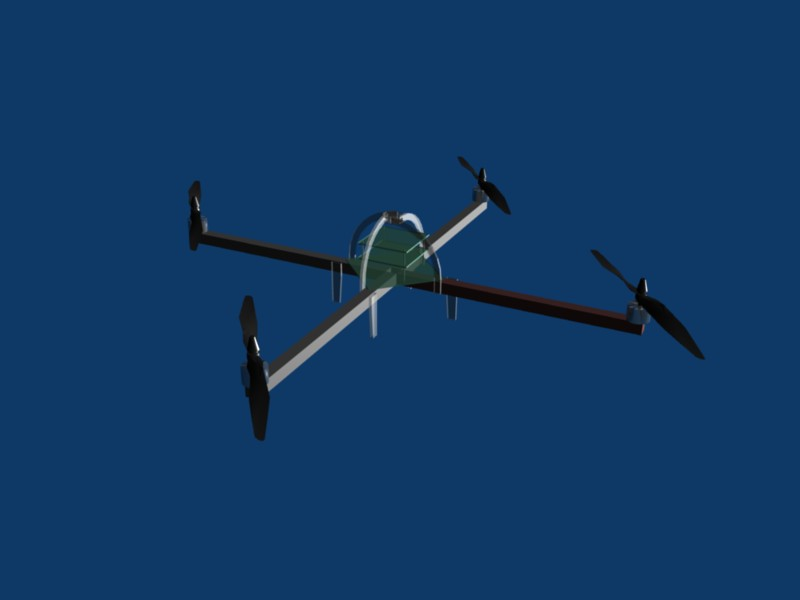
\includegraphics[width=0.4\textwidth]{f31.jpg}
\caption{四旋翼模型}
\label{fig28}
\end{figure}

最后启动 FlightGear 进行调试。在终端窗口内,输入'fgrun',启动 FlightGear 软件,选择“Quadrotor”,选择“next” 设置好飞机场、飞行时间等参数后,点击“run”按钮,如图\ref{fig29}所示。如果顺利进入了图 \ref{fig30}界面,并且伴随螺旋桨轰鸣声,则说明四旋翼无人机飞行模型已经成功配置到了 FlightGear 中,可以使用动力学模型驱动来进行飞行模拟了。
  \begin{figure}[!ht]
\centering
\subfigure[模型选择界面]{
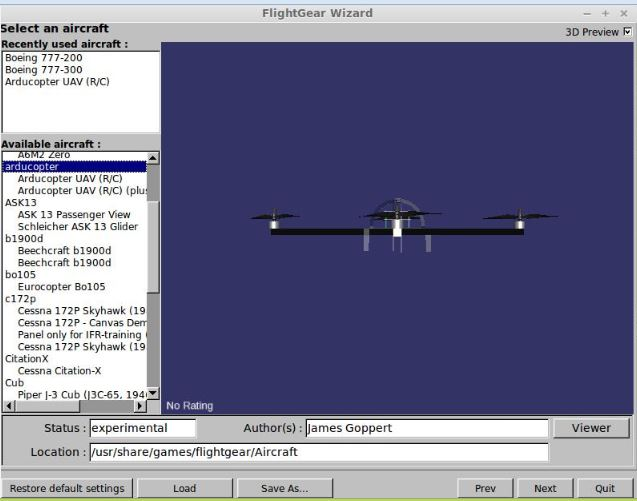
\includegraphics[width=0.45\textwidth]{f32.jpg}\label{f:1}}
\subfigure[机场选择界面]{
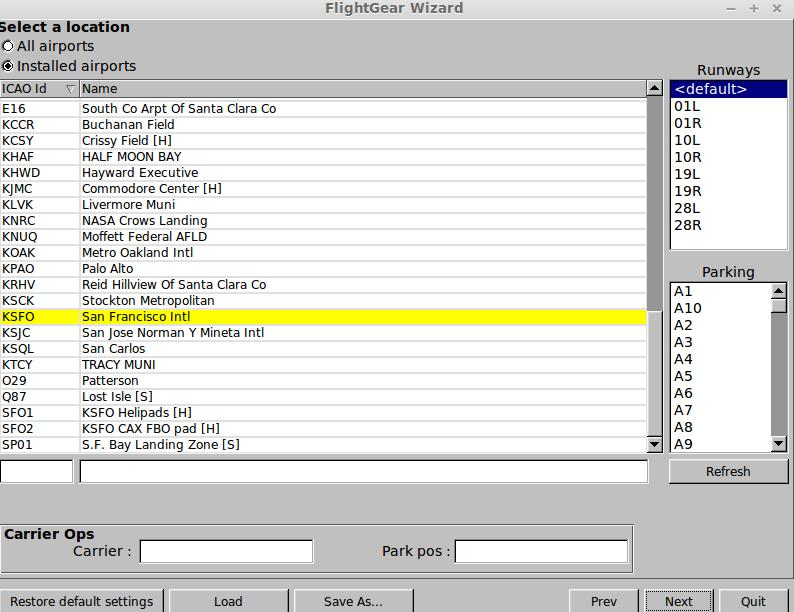
\includegraphics[width=0.45\textwidth]{f27.jpg}\label{f:2}}
\caption{\label{fig29}FlightGear飞行器选择界面}
\end{figure}
\begin{figure}[!ht]
\centering
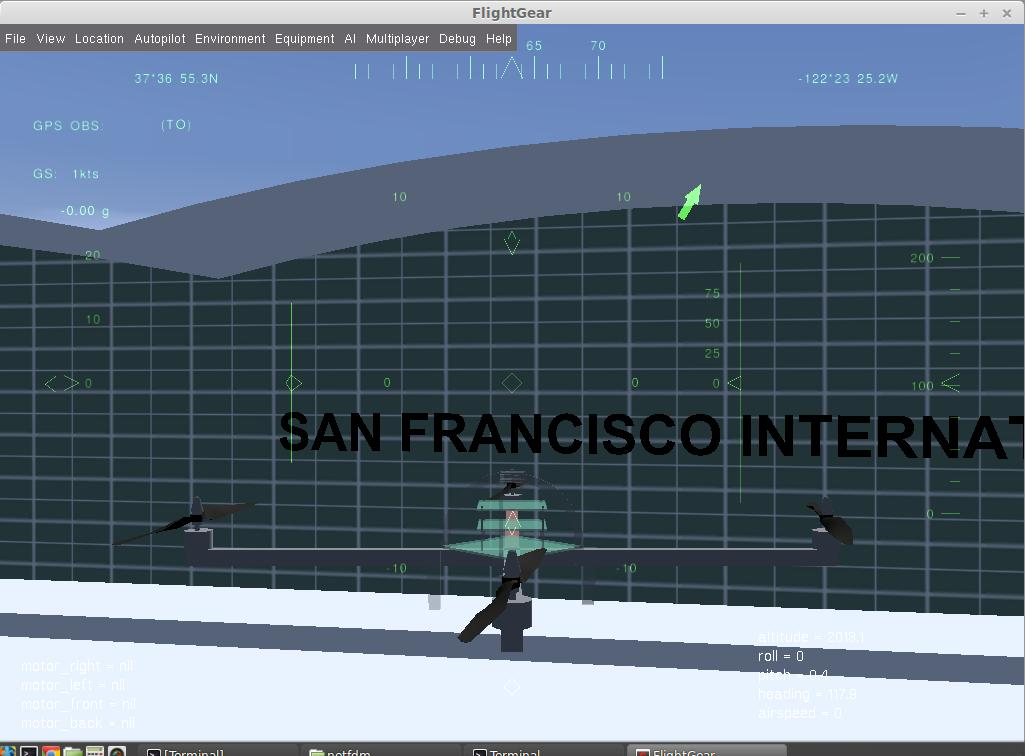
\includegraphics[width=0.8\textwidth]{f40.jpg}
\caption{四旋翼无人机启动界面}
\label{fig30}
\end{figure}
  \item 模型启动

  在完成飞行器模型的部署后,便可以驱动模型进行仿真模拟了。在终端内,输入命令,驱动FlightGear 进行飞行模拟的命令行如下:
\begin{lstlisting}
 fgfs --aircraft=arducopter
      --fdm=network
      --airport=KSFO
      localhost,5501,5502,5503
      --airport=KSFO
 \end{lstlisting}
 --airport=KSFO : 指 定 仿 真 时 使 用 的 飞 机 场 ID , 该 飞 机 场 必 须 在/FlightGear/Airports下能够找到。

 --aircraft=quadrotor:指定仿真时使用的飞行器模型

 --fdm=network:指定仿真使用的动力学模型,可供选择的有:jsb,  larcsim,yasim,  magic,balloon,  external,  pipe, ada,  null。默认的动力学模型是jsb(JSBSim)。network指通过外部数据驱动程序运行(比如通过网络发送的数据)。

  localhost,5501,5502,5503 开启动力学数据连接协议,向fligtgear传送数据。
\end{enumerate}
\subsection{仿真效果}
\begin{figure}[!hbt]
\centering
\subfigure[滚转运动]{
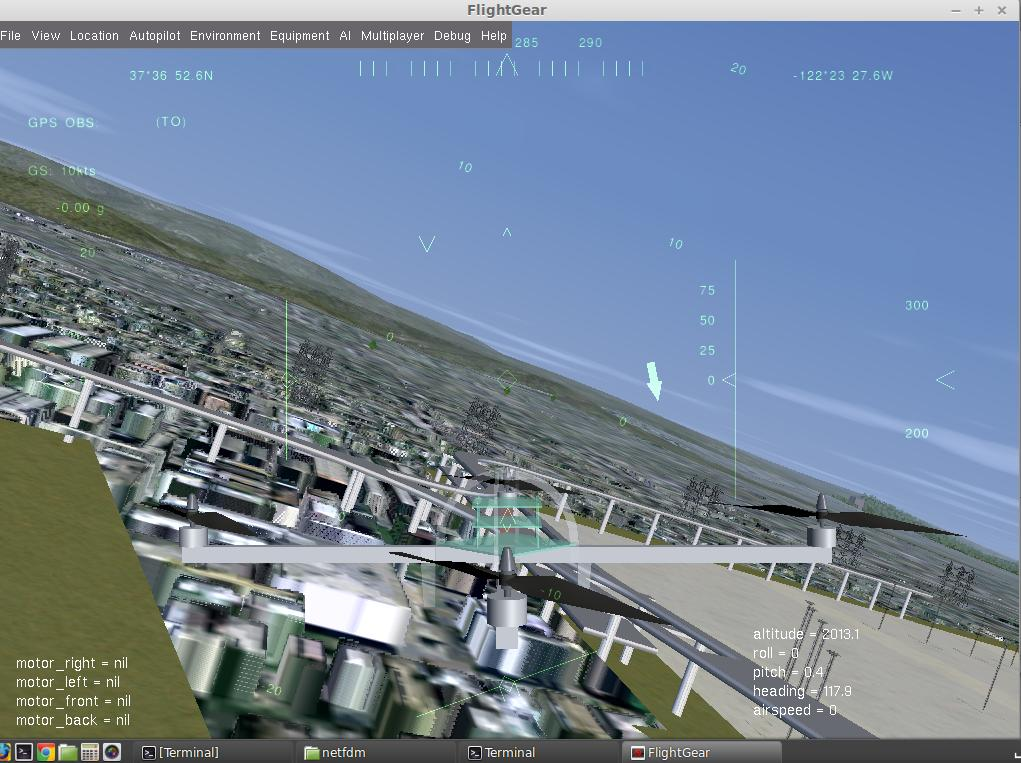
\includegraphics[width=0.4\textwidth]{f41.jpg}\label{f:1}}
\subfigure[俯仰运动]{
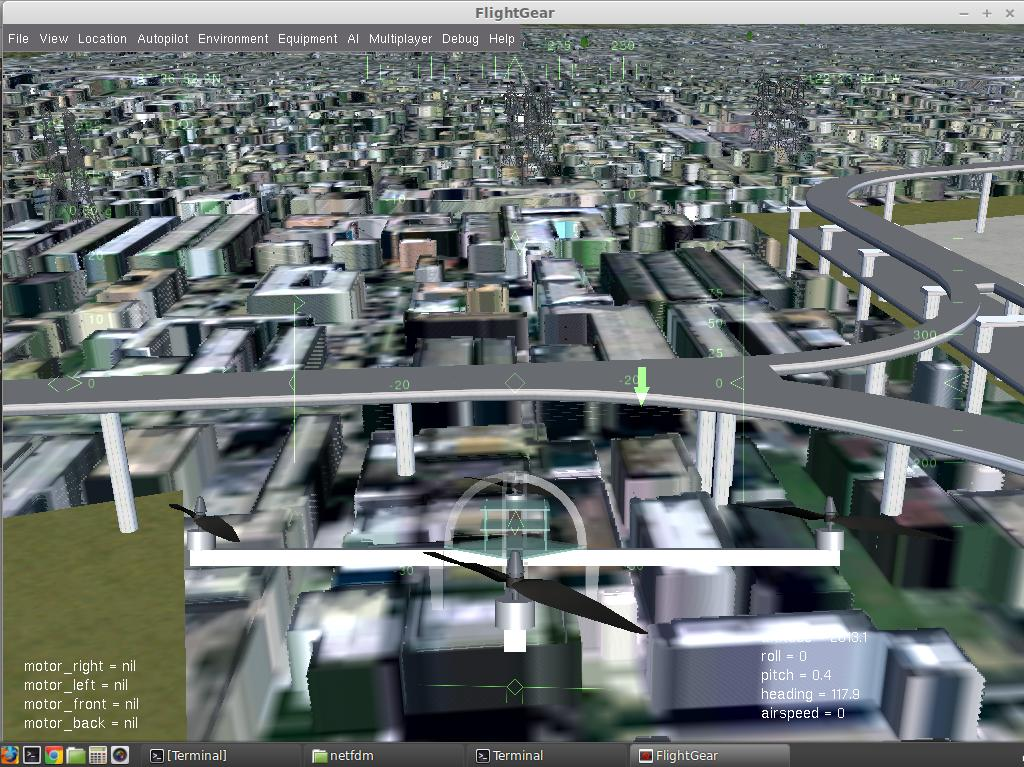
\includegraphics[width=0.4\textwidth]{f42.jpg}\label{f:2}}\\
\subfigure[偏航运动]{
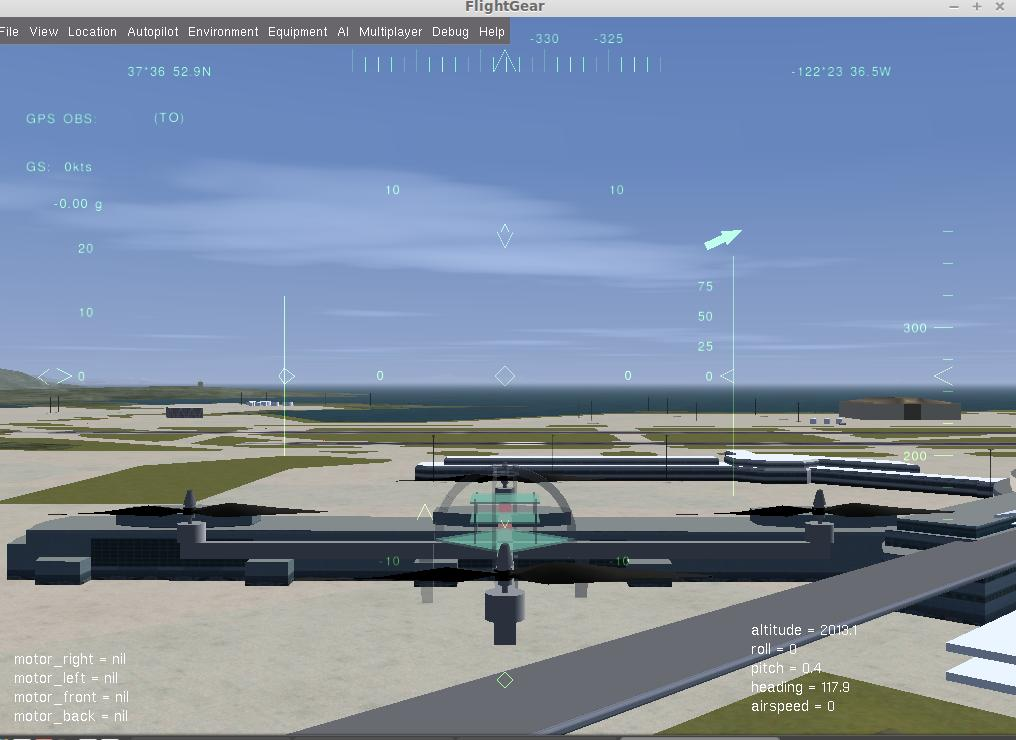
\includegraphics[width=0.4\textwidth]{f43.jpg}\label{f:3}}
\subfigure[空中悬停]{
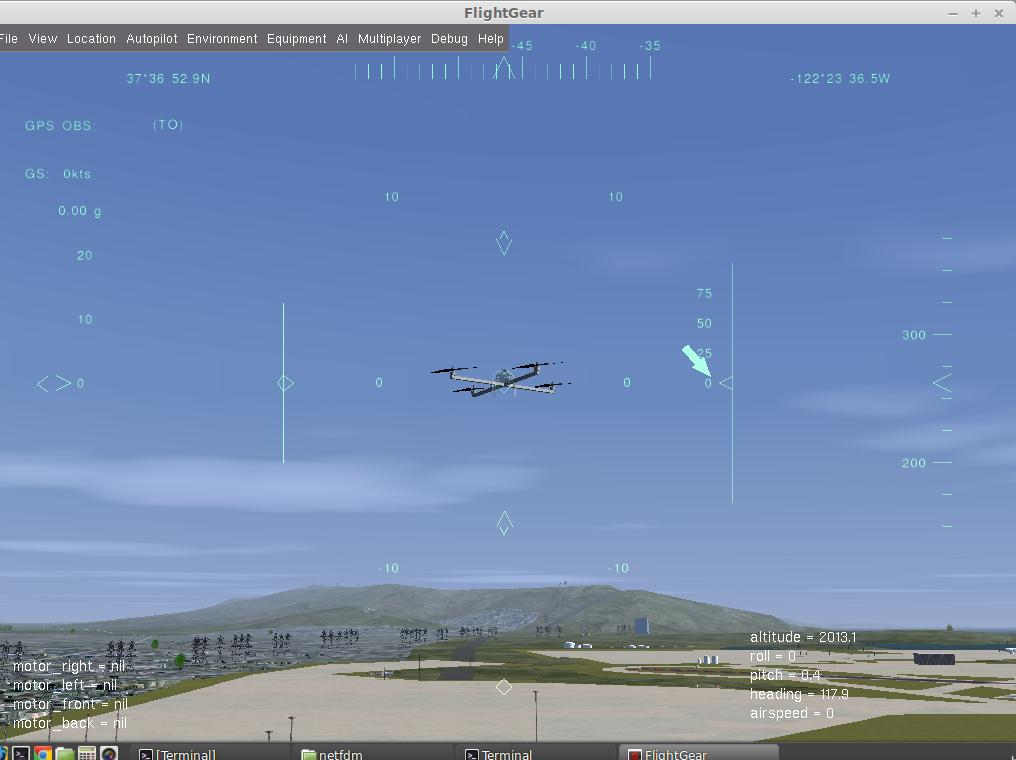
\includegraphics[width=0.4\textwidth]{f44.jpg}\label{f:4}}
\caption{\label{fig31} 四旋翼仿真效果 }
\end{figure}

系统实现了四旋翼无人机飞行的三维可视仿真。将四旋翼无人机的飞行参数(六自由度数据),通过通信模块传递给FlightGear,在飞行参数的驱动下,四旋翼无人机模型在显示屏上可以模拟飞行器起飞、飞行、降落等各种飞行场景,画面连续,可控制播放,可变视角观察(键盘ctrl+V命令),并可进行飞行数据记录与视景回放,达到了设计的预期效果,满足了仿真要求,如图\ref{fig31}所示。
\include{body/simulate}

% 结论
%%%%%%%%%%%%%%%%%%%%%%%%%%%%%%%%%%%%%%%%%%%%%%%%%%%%%%%%%%%%%%%%%%%%%%%%%
%
%   LaTeX File for Doctor (Master) Thesis of Tsinghua University
%   LaTeX + CJK     清华大学博士(硕士)论文模板
%   Based on Wang Tianshu's Template for XJTU
%	Version: 1.00
%   Last Update: 2003-09-12
%
%%%%%%%%%%%%%%%%%%%%%%%%%%%%%%%%%%%%%%%%%%%%%%%%%%%%%%%%%%%%%%%%%%%%%%%%%
%   Copyright 2002-2003  by  Lei Wang (BaconChina)       (bcpub@sina.com)
%%%%%%%%%%%%%%%%%%%%%%%%%%%%%%%%%%%%%%%%%%%%%%%%%%%%%%%%%%%%%%%%%%%%%%%%%

\renewcommand{\baselinestretch}{1.5}
\fontsize{12pt}{13pt}\selectfont

\chapter{总结与展望}\label{conclusion}
\markboth{总结与展望}{总结与展望}
%\addcontentsline{toc}{chapter}{\hei 总结与展望}
\section{全文总结}
飞行控制是保证飞机安全飞行的核心部分,是衡量飞机飞行品质的重要指标。飞行控制技术的高低决定了无人机的飞行品质。本文主要研究了四旋翼无人机及固定翼无人机的飞行控制,基于FLightGear 飞行模拟软件搭建飞行仿真平台,实现半物理仿真。本文主要做的工作如下:
\vspace{-10pt}
\begin{enumerate}
	\item 简述飞行控制过程中坐标系转换的原理以及坐标系旋转矩阵公式推导过程。
	\item 推导四旋翼旋转矩阵,为六自由度四旋翼飞控模型铺垫。
	\item 概述FlighGear软件组件,程序框架及软件优势。
	\item 进行四旋翼无人机的飞控建模,分为三个方面。第一个方面,是实现飞行摇杆的数据传入过程,对于四旋翼而言,主要是飞行姿态角传入及油门数据读取。第二部分,是建立六自由度非线性的飞行动力学模型,实现FlightGear外部飞控模型的实时解算,达到实时控制四旋翼无人机效果。第三部分,是基于FlightGear搭建的三维视景仿真系统的介绍。
	\item 基于FlightGear内部的飞行动力学模型JSBSim,对固定翼无人机进行控制。其过程同样分为三部分,第一部分与第三部分分别于四旋翼无人机相同,主要是第二部分的飞行动力学模型。本文对JSBSim模型进行配置,实现JSBSim与飞行摇杆数据之间的接口通信编程。
	\item 详细讲述FlightGear飞行器驱动的步骤以及系统实施的条件。以四旋翼为对象,从飞行器模型载入到FlightGear通信模块的实现最后到FlightGear三维视景系统的仿真效果展现。介绍了在Linux操作系统下,如何使用FlightGear进行半物理仿真的操作步骤。
	\item 本文对无人机飞行控制的工作作出了一些展望,尤其是基于视觉的无人机飞行控制,结合FlightGear飞行仿真软件,实现功能更为强大的半物理仿真的飞行控制。
\end{enumerate}

\section{对未来工作的展望}
根据本文的分析,可以发现无人机飞行控制技术已经非常成熟,但也存在不少可以改进的地方,基于视觉的无人机飞行控制,可以作为未来研究的重点,概括起来主要有如下几个方面:
\vspace{-10pt}
\begin{enumerate}
\item 可行性。无人机内置水平和竖直两个摄像头,可以完成对无人机所处环境图像的采集,这满足了引入计算机视觉方法的前提条件;
\item 高效性。无人机采集的图像,能够通过无人机内部自建的 wifi无线网络实时传送至计算机,从而可在计算机上运行视觉处理算法,充分发挥计算机强大的计算能力,实现对有用信息进行解算。这是非常关键的一点,解决了计算机视觉方法数据处理量大,难以利用无人机自带的处理器芯片进行求解的问题;
\item 自主飞行性。无人机在实际飞行时,必须由人实时发出控制信号才能保证其飞行。而我们希望无人机在需要很少的人为引导,甚至是没有人干预的情况下,同样可以安全平稳飞行,即减弱人在整个控制系统中所扮演的角色。利用计算机视觉技术取代人在控制系统中的作用,就显得尤为重要。
\item 通用性。摄像机善于捕捉运动信息,而传统的传感器则较吃力,从应用的角度来看,视觉信号的抗干扰性能很好。此外,视觉导航既适用于室内环境,也适用于室外环境,通用性好。
\item 合理性。无人机设计的完整合理性,使我们不需要考虑其电子元件级的实现、气动布局、力学建模以及电机转速的控制方法,可直接通过对俯仰角、滚转角、偏航角以及竖直方向速度的控制实现对无人机的各种控制,这大大简化了我们的工作,使我们可以专注于无人机与计算机视觉方法的结合。

\end{enumerate}


%参考文献
\wuhao

\bibliographystyle{unsrt}

\ifpdf \phantomsection \fi

\addcontentsline{toc}{chapter}{\hei 参考文献}

%\addtolength{\itemsep}{-0.8 em} % 缩小参考文献间的垂直间距, 在bibtex下无效
\bibliography{reference/reference}

% 致谢
%%%%%%%%%%%%%%%%%%%%%%%%%%%%%%%%%%%%%%%%%%%%%%%%%%%%%%%%%%%%%%%%%%%%%%%%%
%
%   LaTeX File for Doctor (Master) Thesis of Tsinghua University
%   LaTeX + CJK     清华大学博士(硕士)论文模板
%   Based on Wang Tianshu's Template for XJTU
%   Version: 1.00
%   Last Update: 2003-09-12
%
%%%%%%%%%%%%%%%%%%%%%%%%%%%%%%%%%%%%%%%%%%%%%%%%%%%%%%%%%%%%%%%%%%%%%%%%%
%   Copyright 2002-2003  by  Lei Wang (BaconChina)       (bcpub@sina.com)
%%%%%%%%%%%%%%%%%%%%%%%%%%%%%%%%%%%%%%%%%%%%%%%%%%%%%%%%%%%%%%%%%%%%%%%%%


%%%%%%%%%%%%%%%%%%%%%%%%%%%%%%%%%%%%%%%%%%%%%%%%%%%%%%%%%%%%%%%%%%%%%%%%%
%
%   LaTeX File for phd thesis of xi'an Jiao Tong University
%
%%%%%%%%%%%%%%%%%%%%%%%%%%%%%%%%%%%%%%%%%%%%%%%%%%%%%%%%%%%%%%%%%%%%%%%%%
%   Copyright 2002  by  Wang Tianshu    (tswang@asia.com)
%%%%%%%%%%%%%%%%%%%%%%%%%%%%%%%%%%%%%%%%%%%%%%%%%%%%%%%%%%%%%%%%%%%%%%%%%
\renewcommand{\baselinestretch}{1.5}
\fontsize{12pt}{13pt}\selectfont

\chapter*{致~~~~谢}
\markboth{致谢}{致谢}
\addcontentsline{toc}{chapter}{\hei 致谢}
首先要感谢我的导师布树辉老师。感谢布老师在整个毕设过程中的耐心指导,感谢布老师在整个论文进展过程中,提供的文献资料和实验平台,感谢布老师在整个毕设过程中的宝贵意见。与布老师交流过程中,不断的加深对问题的理解与认识,不断的提高自己解决问题的能力。对于很多女同学而言,并不会去选择编程方向作为自己的毕设,我只是因为一时的兴趣才去选择了它。回想起来,自己从一月份的一无所知到三月份的懵懵懂懂再到如今六月份的豁然开朗,从开始的压力山大到中途的排斥抵触再到现在的一往无前,在布老师的悉心教导下,让我懂得科研的路途毕竟是曲折而坎坷的,需要一份对待科研的严谨与热情,去迎风破浪,最终,必会柳岸花明。

同时要感谢教研室的赵勇师兄,在坐标系变换的编程实践中,赵勇师兄提供的四元数算法,让问题瞬间豁然开朗,感谢赵勇师兄的不吝赐教。感谢韩鹏程,程少光,王磊师兄,在我代码调试过程中,悉心的指导,在我压力很大的时候,热心的开导,分享他们的科研经历,感谢你们的鼓励与支持,让我可以一步一步慢慢的成长。

另外要感谢Curt Olson等飞行爱好者们,是他们创造了FlightGear这个功能强大的开源的飞行模拟软件;感谢为Linux贡献代码的程序员们,这个自由免费的平台为我完成毕设提供了不少便利;感谢清华大学王磊博士,他创作的\LaTeX 模板使我的论文的排版得以顺利完成。

最后感谢我的家人对我一如既往的关心和支持,感谢我的男朋友对我一如既往的支持与鼓励。

\chapter*{毕业设计小结}
\markboth{毕业设计小结}{毕业设计小结}
\addcontentsline{toc}{chapter}{\hei 毕业设计小结}

本次毕业设计不仅仅是对我大学四年来学习知识的一个总结,更是对我知识学习能力一次拓展与提高的过程。本次毕设主要以四旋翼无人机飞行控制为核心,学习了如何通过C++编程实现坐标系的转换,旋转矩阵的运算。实践了通过编程实现半物理仿真的过程,以及提高了如何将数学公式转换为编程语言的能力。同时,了解了FlightGear飞行模拟软件的通信过程,学习如何实现UDP的通信编程。因为FlightGear 是一款功能强大的开源软件,更适合在Linux操作系统下进行使用,所以,学习了如何在Liunx操作系统下进行FlightGear软件的安装,启动及shell 文件的编写。在Linux系统下,更方便的使用FlightGear飞行模拟软件与Joystick摇杆结合,实现对四旋翼无人机的飞行控制。同时,本次毕设也对固定翼无人机的飞行控制进行了学习,通过FlightGear自带的JSBsim飞行动力学模型,结合Joystick飞行摇杆,通过TCP/IP编程实现对FlightGear的通信过程,完成对固定翼无人机的飞行控制。

本次毕业设计中印象比较深刻的有飞行控制过程中,坐标系转换的问题,必须保证坐标系选择的一致性,学习了如何通过C++编程实现对向量矩阵的运算过程。同时,通过对FlightGear通信模块的学习,了解了UDP,TCP/IP协议,通过C++编程实现Joystick飞行摇杆数据到FlightGear通信的过程。对六自由度非线性飞行动力学方程的推导过程,进行了十分深刻的了解。同时,对如何将数学公式变成编程语言的编程能力,有了一定提高。

经历了本次毕设,我对无人机飞行控制的过程有了一定了解,对Linux操作系统有了一定认识。在今后的学习过程中,会更加深入的学习飞行控制理论,提高自己的编程水平,熟练使用FlightGear飞行模拟软件,实现功能更强大的飞行仿真。




%  附录

%\begin{appendix}
%    \renewcommand{\chaptername}{附录\Alph{chapter}}
%   \chapter*{附~~录}
\markboth{附录}{附录}
\addcontentsline{toc}{chapter}{\hei 附录}
\noindent\bfseries\texttt{test.py}源代码:
\setmonofont{Monaco}
\lstset{basicstyle=\ttfamily\scriptsize,keywordstyle=\color{blue},commentstyle=\color{green},stringstyle=\color{red},tabsize=4,frameround=fttt,escapeinside=``,lineskip=0.6pt}
\begin{lstlisting}[language=Python]
#!/usr/bin/env python
from TOSSIM import *
from random import *
import sys

if len(sys.argv) < 3:
	print "usage: need 2 parameter, nodes number and simulate time"
	sys.exit(0)

nodes = int(sys.argv[1])
sim_time = int(sys.argv[2])
t = Tossim([])
r = t.radio()

f = open("topo.txt", "r")
lines = f.readlines()
for line in lines:
  s = line.split()
  if (len(s) > 0):
    if s[0] == "gain":
      r.add(int(s[1]), int(s[2]), float(s[3]))

noise = open("meyer-short.txt", "r")
lines = noise.readlines()
for line in lines:
  str = line.strip()
  if (str != ""):
    val = int(str)
    for i in range(0, nodes):
      m = t.getNode(i);
      m.addNoiseTraceReading(val)

for i in range(0, nodes):
  m = t.getNode(i);
  m.createNoiseModel();
  time = randint(t.ticksPerSecond(), 10 * t.ticksPerSecond())
  m.bootAtTime(time)
  print "Booting ", i, " at time ", time

print "Starting simulation."

t.addChannel("Forwarder", sys.stdout)
t.addChannel("TestNetworkC", sys.stdout)
t.addChannel("TreeRouting", sys.stdout)
t.addChannel("LI", sys.stdout)

while (t.time() < sim_time):
  t.runNextEvent()

print "Completed simulation."
\end{lstlisting}

\noindent\bfseries\texttt{ctpsim-3d.py}源代码:
\begin{lstlisting}[language=Python,tabsize=2]
#!/usr/bin/env python
import xmlrpclib,time
import re

nodes = 10
server = xmlrpclib.Server('http://localhost:20738/RPC2')
G = server.ubigraph

G.clear()

node = [0 for col in range(nodes)]

for i in range(0,nodes):
	node[i] = G.new_vertex()
	G.set_vertex_attribute(node[i], 'label', str(i))
	G.set_vertex_attribute(node[i], 'shape','sphere')
	G.set_vertex_attribute(node[i], 'size','0.5')
	G.set_vertex_attribute(node[i], 'color','#1E90FF')

edge = [[0 for col in range(nodes)] for row in range(nodes)]

for i in range(0,nodes):
	for j in range(i+1, nodes):
		edge[i][j] = G.new_edge(node[i], node[j])
		edge[j][i] = edge[i][j]

topo = open('topo.txt', 'r')
lines = topo.readlines()
for line in lines:
	s = line.split()
	if s[0] == 'gain':
		if int(s[1]) < nodes and int(s[2]) < 
				nodes and int(s[1]) < int(s[2]):
			G.set_edge_attribute(edge[int(s[1])][int(s[2])],
					     'strength',
					     str(1 + float(s[3]) / 120.0))
			#G.set_edge_attribute(edge[int(s[1])][int(s[2])],
					      'label', s[3]) # add gain value

G.set_vertex_attribute(node[0], 'color', '#FFFF00') # root node

def node_spark(node_id):
	node_id = int(node_id)
	G.set_vertex_attribute(node[node_id], 'color', '#FF0000')
	G.set_vertex_attribute(node[node_id], 'color', '#FFFFFF')
	G.set_vertex_attribute(node[node_id], 'color', '#FF0000')
	G.set_vertex_attribute(node[node_id], 'color', '#FFFFFF')
	if node_id != 0:
		G.set_vertex_attribute(node[node_id], 'color', '#1E90FF')
	else:
		G.set_vertex_attribute(node[node_id], 'color', '#FFFF00')


def node_display_debug_str(node_id, debug_str):
	G.set_vertex_attribute(node[int(node_id)], 'label', node_id+": "+debug_str)
	#time.sleep(0.0)
	#G.set_vertex_attribute(node[node_id], 'label', str(node_id))

def process_boot_at_time(node_id, time):
	G.set_vertex_attribute(node[int(node_id)], 'label','boot at:'+time)


def process_parent_change(node_id, origin_parent, new_parent):
	node_id = int(node_id)
	origin_parent = int(origin_parent)
	new_parent = int(new_parent)
	if origin_parent != 65535:
		G.set_edge_attribute(edge[node_id][origin_parent], 'color', '#C0C0C0')
		G.set_edge_attribute(edge[node_id][origin_parent], 'width','1')
	G.set_edge_attribute(edge[node_id][new_parent], 'color', '#FF00FF')
	G.set_edge_attribute(edge[node_id][new_parent], 'width','7')
	time.sleep(0.5)

def animateArrow(e, reverse):
  pos = 0.0
  if reverse:
    pos = 1.0
  G.set_edge_attribute(e, "arrow_position", str(pos))
  G.set_edge_attribute(e, "arrow_reverse", str(reverse))
  G.set_edge_attribute(e, "arrow", "true")
  for i in range(0,20):
    a = i / 19.0
    if reverse:
      a = 1.0 - a
    G.set_edge_attribute(e, "arrow_position", str(a))
    time.sleep(0.05)
  G.set_edge_attribute(e, "arrow", "false")

def animate_broadcast(node_id):
	node_id = int(node_id)
	for j in range(2):
		for i in range(21):
			G.set_vertex_attribute(node[node_id], 
				'size', str(0.5 + i / 20.0))
		for i in range(21):
			G.set_vertex_attribute(node[node_id],
				'size', str(0.5 + (20 - i)/20.0))

def process_send_beacon(node_id):
	node_id = int(node_id)
	animate_broadcast(node_id)
	

def process_forwoard_subsend(node_id, dest):
	print node_id, dest
	node_id = int(node_id)
	dest = int(dest)
	if node_id == dest:
		return
	G.set_edge_attribute(edge[node_id][dest], 'arrow','true')
	if node_id > dest:
		G.set_edge_attribute(edge[node_id][dest], "arrow_reverse", 'true')
	speed = 10 # the smaller, the faster
	for pos in range(speed+1):
			if node_id < dest:
				G.set_edge_attribute(edge[node_id][dest], 
					"arrow_position", str(pos / float(speed)))
			else:
				G.set_edge_attribute(edge[node_id][dest], 
					"arrow_position", str(1- pos / float(speed)))
			time.sleep(0.05)
	G.set_edge_attribute(edge[node_id][dest], "arrow_reverse", 'false')
	G.set_edge_attribute(edge[node_id][dest], 'arrow','false')

def dispatch_each_line(line):
	re_boot_at_time = r'Booting  (/d+)  at time  (/d+)'
	re_debug = r'^DEBUG \((\d+)\): (.*)'

	re_parent_change = r'Changed parent. from (\d+) to (\d+)'
	# 1.parent,  2.etx
	re_send_beacon = r'CtpRoutingEngineP\$0\$sendBeaconTask\$runTask parent: (\d+) etx: (\d+)' 
	# 1.dest, 2. error
	re_forward_subsend = r'CtpForwardingEngineP\$0\$SubSend\$sendDone to (\d+) and (\d+)' 

	match = re.match(re_boot_at_time, line)
	if match:
		process_boot_at_time(match.group(1), match.group(2))
	else:	# match debug messages
		match = re.match(re_debug, line)
		if match:
			node_id = match.group(1)
			node_spark(node_id)
			debug_str = match.group(2)
			node_display_debug_str(node_id, debug_str)
			
			if re.match(re_parent_change, debug_str):
				match = re.match(re_parent_change, debug_str)
				process_parent_change(node_id, match.group(1), match.group(2))
			elif re.match(re_send_beacon, debug_str):
				process_send_beacon(node_id)
			elif re.match(re_forward_subsend, debug_str):	# Forwarder send a packet
				match = re.match(re_forward_subsend, debug_str)
				process_forwoard_subsend(node_id, match.group(1))
line = raw_input()
while line:
	dispatch_each_line(line)
	line = raw_input()
\end{lstlisting}

%\end{appendix}

% 发表的文章列表

%\include{appendix/publications}

\clearpage
\end{document}

%%%%%%%%%%%%%%%%%% End of the file  %%%%%%%%%%%%%%%%%%%%%%%%
